%%%      1         2         3         4         5         6         7        8
%%% 567890123456789012345678901234567890123456789012345687901234567890123456790
%%%

\svnInfo $Id$

\newcommand\schema[1]{\ensuremath{\mathcal{#1}}}
\newcommand\relation[1]{\ensuremath{\textnormal{\bf\textsf{#1}}}}

\makeatletter
\newcommand\skyline{\mathop{\operator@font skyline}\nolimits}
\newcommand\skyband{\mathop{\operator@font skyband}\nolimits}
\makeatother

\newcommand\imp{\Rightarrow}
\newcommand\bigland{\bigwedge}
\newcommand\biglor{\bigvee}
\newcommand\union{\cup}
\newcommand\bigunion{\bigcup}
\newcommand\intersection{\cap}
\newcommand\difference{\backslash}
%\newcommand\dominates{\ensuremath{\succ}\xspace}
%\newcommand\dominatedby{\ensuremath{\prec}\xspace}
%\newcommand\weakdominates{\ensuremath{\succeq}\xspace}
\newcommand\dominates{\ensuremath{\vartriangleright}\xspace}
%\newcommand\notdominates{\ensuremath{\ntriangleright}\xspace}
\newcommand\dominatedby{\ensuremath{\vartriangleleft}\xspace}
%\newcommand\notdominatedby{\ensuremath{\ntriangleleft}\xspace}
\newcommand\weakdominates{\ensuremath{\trianglerighteq}\xspace}
%\newcommand\notweakdominates{\ensuremath{\ntrianglerighteq}\xspace}
\newcommand\weakdominatedby{\ensuremath{\trianglelefteq}\xspace}
%\newcommand\notweakdominatedby{\ensuremath{\ntrianglelefteq}\xspace}
\newcommand\incomparable{\ensuremath{\parallel}\xspace}
\newcommand\comparable{\ensuremath{\perp}\xspace}
%\newcommand\nondistinct{\ensuremath{\doteq}\xspace}
%\newcommand\nondistinct{\ensuremath{\triangleq}\xspace}
%\newcommand\nondistinct{\ensuremath{\stackrel{\vartriangleright}{\thicksim}}\xspace}
\newcommand\nondistinct{\ensuremath{\stackrel{\vartriangleright}{=}}\xspace}


\newcommand\inlinesql[1]{{\tt #1}}
\newcommand\srcref[1]{{\tt #1}}
\newcommand\postgresdocu[2]{\href{http://www.postgresql.org/docs/8.3/static/#1}{#2}\footnote{\url{http://www.postgresql.org/docs/8.3/static/#1}}}
\newcommand\ttbackslash{{\char92}}
\newcommand\ttdolar{{\char36}}
\newcommand\ttspace[1]{{\hbox to #1em{\hfil}}}%

\newtheorem{definition}{Definition}
\newcommand*\definitionautorefname{Definition}
\newtheorem{lemma}{Lemma}
\newcommand*\lemmaautorefname{Lemma}
\newtheorem{theorem}{Theorem}
%\newcommand*\theoremautorefname{Theorem}
\newtheorem{example}{Example}
\newcommand*\exampleautorefname{Example}
\newtheorem{property}{Property}
\newcommand*\propertyautorefname{Property}

\newcommand\nt[1]{\textit{#1}}

\makeatletter
\newcommand\ellipsis{\textcolor{blue}{\ensuremath{[\ldots]}}}%

\newenvironment{interactive}
{%
\newcommand\shprompt[1]{\$\ {\textbf{##1}}}
\newcommand\sqlprompt[1]{db=\# {\textbf{##1}}}
\newcommand\sqlpromptcont[1]{db-\# {\textbf{##1}}}
\newcommand\comment[1]{{\rmfamily\textit{##1}}}
\newcommand\rcomment[1]{\hfill\comment{##1}}
\newcommand\commentskip{{\vspace{3pt}}}
%\newcommand\prebreak{\hbox to 1em{\textcolor{blue}{\ensuremath{\hookleftarrow}}}}
%\newcommand\postbreak{\hbox to 1em{\textcolor{blue}{\ensuremath{\hookrightarrow}}}}
\newcommand\prebreak{\textcolor{blue}{\ensuremath{\hookleftarrow}}}
\newcommand\postbreak{ \kern-1em\hbox to 1em{\textcolor{blue}{\ensuremath{\rightarrow}}\hss}}
\begingroup\small\list{}{\listparindent 0\p@\itemindent\listparindent\leftmargin15\p@\rightmargin15\p@}\item[]\begin{alltt}}{\end{alltt}\endlist\endgroup}

\newdimen\onecolumnwidth
\global\onecolumnwidth\textwidth
\advance\onecolumnwidth -\columnsep
\divide\onecolumnwidth\tw@
\newsavebox\tempbox

%\newtheoremstyle{sql}% name
%     {\topsep}%      Space above
%     {\topsep}%      Space below
%     {\ttseries}%         Body font
%     {}%         Indent amount (empty = no indent, \parindent = para indent)
%     {\bfseries}% Thm head font
%     {}%        Punctuation after thm head
%     {\newline}%     Space after thm head: " " = normal interword space;
%           %       \newline = linebreak
%     {...}%         Thm head spec (can be left empty, meaning `normal')
%\newtheorem{sql}{SQL}[subsection]

%\newtheormstyle{sql}{\topsep}{\topsep}{
\newenvironment{sql}{%
\list{}{%
    \refstepcounter{equation}%
    \listparindent 0\p@
    \itemindent\listparindent
    \leftmargin15\p@
%    \rightmargin15\p@
    \parsep \z@ \@plus\p@
    \tt
 }%
\item[]%
}{%
\hfill\hbox{{\normalfont\normalcolor(\theequation)}}%
\endlist
}%

\makeatother

\newcommand\subplotprofile[2][todo]{%
\subfloat[#1]{%
\includegraphics[width=\onecolumnwidth]{plots-profile/#2}}%
}%

\newcommand\subplotlabeledprofile[3]{%
\subfloat[#1]{%
\includegraphics[width=\onecolumnwidth]{plots-profile/#2}%
\label{#3}%
}}%

\lstdefinelanguage{pseudo}{
	language=C,
	mathescape=true, 
	literate={:=}{{$\gets$}}1, 
	morekeywords={function,foreach,forever,bool,true,false}
}

\newcommand\nospellcheck[1]{#1}%
\newcommand\naive{\nospellcheck{na\"{\i}ve}\xspace}%
\newcommand\Naive{\nospellcheck{Na\"{\i}ve}\xspace}%


%%%
%%% CHAPTER: Introduction
%%%



\chapter{Introduction}
\label{chap:introduction}

\section{General Introduction}
\label{sec:generalintroduction}

In everyday-life we are used to making decisions based on multiple
criteria, e.g. price and quality for products.  Frequently there is no
clear winner over all criteria, i.e. a high-priced product with high
quality and a cheap product with lower quality.  Surely we are not
interested in a product with a high price and poor quality, we will
later refer this situation as \emph{this product is dominated by
another one}, as there are others which better fulfill our criteria.  The
products which are not dominated are more or less equally good based on
our given criteria, and we need to apply more criteria to come to a
decision.  These products are called to be \emph{Pareto optimal}
based on the given criteria. \citet{Borzsonyi2001} coined in their
paper the term \emph{skyline operator} for this type of queries.

\begin{figure}[htbp]
% this is from: 
% http://www.istockphoto.com/file_closeup/where/scenics/cityscapes/
% 2358169_lightning_traffic_over_danube_bridge_and_vienna_skyline.php
% ?id=2358169
%
% Photographers Description:
%
% viennese skyline with cars driving on a street shot by night with a
% long time exposure. I added high contrast, therefore image gets very
% little grainy.
%
\centering
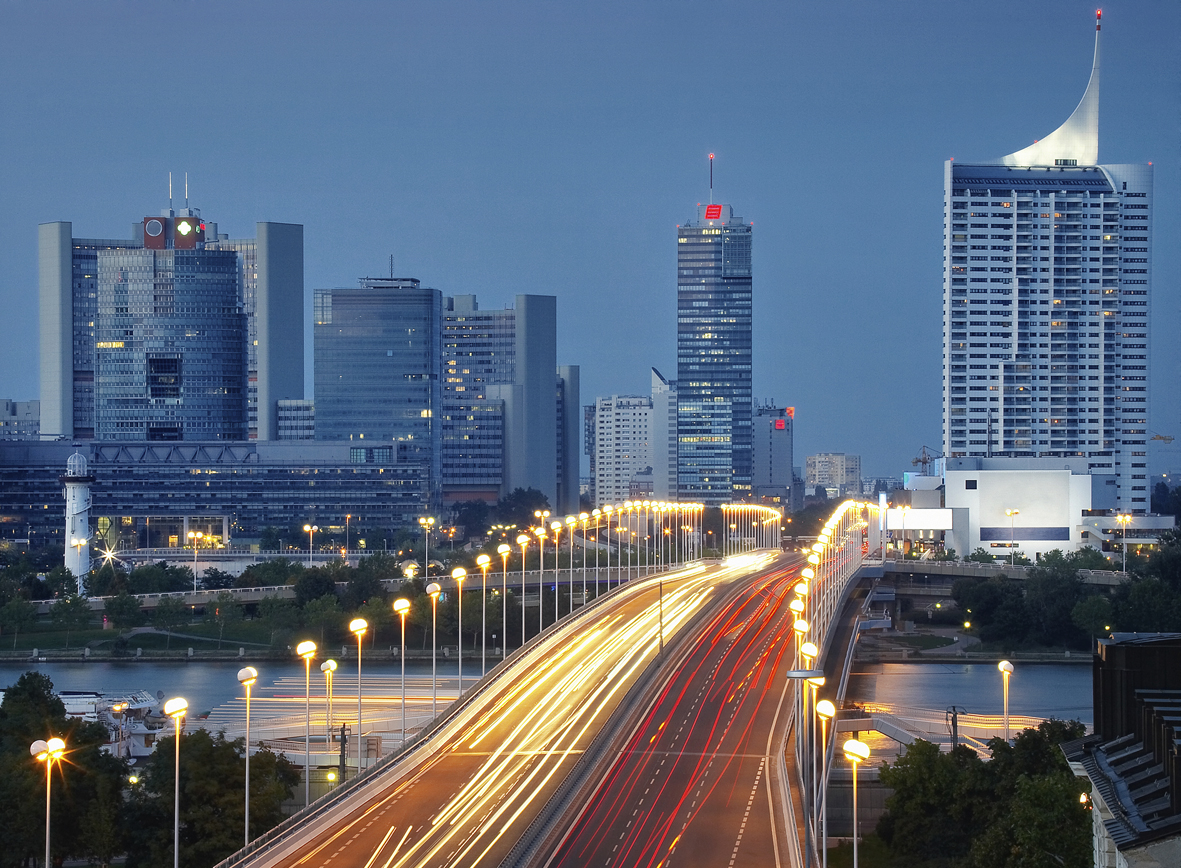
\includegraphics[scale=1.0]{photos/iStock_000002358169Large_100mm}%
\caption{Viennese skyline (nightshot with long exposure time, 
taken by Franz Pfl\"ugl / Vienna)}%
\label{fig:vienneseskyline}%
\end{figure}

When thinking of the term \emph{skyline}, images like 
\autoref{fig:vienneseskyline} might come to our mind.
The popularity of such photographs is illustrated by following figures:
\emph{Google images} returns $\approx 3{,}580{,}000$ hits, not
counting the hits for the Nissan's skyline sports car, for the search
term
\emph{skyline -nissan}, and 
%
\href{http://www.istockphoto.com/}{istockphoto.com}, 
a popular website with a collection of member-generated royalty-free images,
has $\approx 25{,}000$ photos in stock for the search term
\emph{skyline}, as of May 23 2008. 
% http://www.merriam-webster.com/cgi-bin/dictionary?book=Dictionary&va=skyline
The Merriam-Webster's online dictionary gives following definition for \emph{skyline}:
\begin{enumerate}
\item the apparent juncture of earth and sky: \emph{horizon}
\item an outline (as of buildings or a mountain range) against the
background of the sky
\end{enumerate}

From a more abstract point of view a skyline is made up of objects
(buildings, mountains and such) which do not have another object
closer and taller to the eye of the beholder. If we are only
interested in the objects that are ``touching the sky'', we consider
only the tallest object in each direction of view. On the other hand
if we care about visibility, an object is visible as long as there is
no object closer and taller. We ask the alert reader to excuse the
simplifications we made here, the authors are aware of the concept of
perspective projection and of the fact that the earth is not a disk.
%However, we will shortly see how this intuition matches a precise
%mathematical definition and a concept in the real of databases.

\bigskip
In the realm of database systems the \emph{skyline operator} is
important for supporting multi-criteria decision making applications.
Given a set of $d$-dimensional data points, the \emph{skyline}
consists of those points, called \emph{skyline points}, which are not
\emph{dominated} by any other data points. One data point $r$ dominates
another data point $s$ if it is at least as good as $s$ in all
dimensions and better in at least one.
\citet{Borzsonyi2001} proposed a {\em skyline} extension of the SQL
syntax with this form:

\begin{sql}
SELECT ... FROM ... WHERE ... \\
GROUP BY ... HAVING ...       \\
SKYLINE OF \textnormal{[}DISTINCT\textnormal{]} $a_1$ \textnormal{[}MIN$|$MAX$|$DIFF\textnormal{]}, ..., $a_m$ \textnormal{[}MIN$|$MAX$|$DIFF\textnormal{]} \\
ORDER BY ...
\end{sql}

Computing the skyline is also known as the \emph{maximum vector
problem} \citep{Kung1975, Preparata1985}. The terms \emph{skyline} and
\emph{skyline operator} in the realm of databases were coined by
\citet{Borzsonyi2001}. The following examples give a motivation why 
\emph{skyline operator} is a good name for this type of
\emph{preference queries}, they also illustrate the usage of the
\inlinesql{DIFF} and \inlinesql{DISTINCT} keyword.

In \autoref{fig:threeDskyline} the yellow arrow indicates the
direction of view and the colored cuboids illustrate
buildings. \autoref{tab:threeDskyline} shows the coordinates of the
lower left edge of each building and gives them names ($a, b,
\ldots$). The same color indicates the same $x$ coordinate. For $y$ we
have only two cases, \emph{front} and
\emph{back}.

\begin{example}[Which buildings are touching the sky?]\label{ex:touchsky}
For sure building $c$ (the green one in the background) and building $f$
(the blue one in the foreground) are part of the answer and $d$ and $e$
are not.  As $a$ and $b$ do have the same height, we could take them
both or make an arbitrary choice among $a$ and $b$.  We will later
see that this taking both or choosing an arbitrary one can be
influenced by the keyword \inlinesql{DISTINCT}. So overall, possible
answers are $\{a, c, f\}$, $\{b, c, f\}$, or $\{a, b, c, f\}$.
\end{example}

\begin{figure}[htbp]
\centering
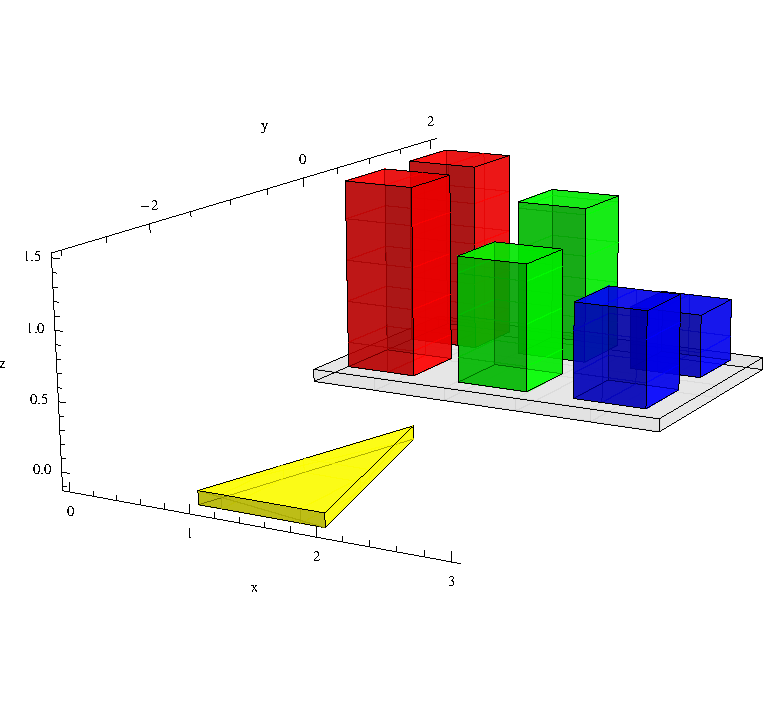
\includegraphics[width=100mm]{plots-misc/PlotSkyline3D}%
\caption{Skyline of buildings}%
\label{fig:threeDskyline}%
\end{figure}

\begin{table}[htbp]
\centering
\begin{tabular}{l|rrrll}
id & x & y & z & color & row\\
\hline
$a$ & 0 & 1 & 1.5 & red & back \\
$b$ & 0 & 0 & 1.5 & red & front \\
$c$ & 1 & 1 & 1.25 & green & back \\
$d$ & 1 & 0 & 1.0 & green & front \\
$e$ & 2 & 1 & 0.5 & blue & back \\
$f$ & 2 & 0 & 0.75 & blue & front
\end{tabular}
\caption{Data for \autoref{fig:threeDskyline}}
\label{tab:threeDskyline}
\end{table}

\begin{example}[Which buildings are visible?]\label{ex:visibility}
To answer this question we also have to take into account how close a
building is, i.e. the $y$ coordinate.  Building $a$ is covered by $b$
and $e$ by $f$, we will later call this property \emph{dominance}. It
is obvious that $c$ and $d$ are part of the answer. The complete
answer is $\{b, c, d, f\}$.
\end{example}

\noindent
The question from \autoref{ex:touchsky} could be formalized in the
following way:

\begin{interactive}
SELECT * FROM building SKYLINE OF x DIFF, z MAX;
\end{interactive}

\noindent
in above query $a$ and $b$ will be part of the answer, whereas in the following
it is up to the database system to make a choice between $a$ or $b$, as they 
are equally good:

\begin{interactive}
SELECT * FROM building SKYLINE OF DISTINCT x DIFF, z MAX;
\end{interactive}

\noindent
On the other hand the query for \autoref{ex:visibility} looks like:

\begin{interactive}
SELECT * FROM building SKYLINE OF x DIFF, y MIN, z MAX;
\end{interactive}

\section{Why extending SQL?}
The skyline operator is within the expressive power of SQL and in
\autoref{sec:rewrite-to-sql} we show how to rewrite an SQL query with
a \inlinesql{SKYLINE~OF}-clause into standard SQL. 
However there are good reasons for including a \emph{skyline} or 
\emph{preference operator} into SQL:

\begin{itemize}
\item 
From a user's perspective, it is easier to specify and easier to grasp
what's going on, than a query with a correlated subquery or using
SQL's \inlinesql{EXCEPT} (see \autoref{sql:rewrite-with-except}).

\item
It is faster to evaluate, as there are numerous algorithms for skyline
queries. Furthermore when this preference query is with a correlated
subselect it boils down to a \naive ``nested-loop'' and
\citet{Grust1997, Braumandl1998} show that such a query cannot be
unnested.

\item
The study of preference queries on their own gave birth to a new set
of optimization opportunities \citep{Chomicki2003a, Kiessling2003}.
\end{itemize}

% \subsection{Fields of Application}
% motivation: green computing: less CPU time,
% less computers, less energy --> safe the planet
% 
% stocks: risk vs. costs (--> streaming skyline see [Tao2006])
% 
% example of skyline
% 
% when traveling by airplane: time vs. costs
% 
% TODO: more dim: \#stops, total dist travel by bus: \#of visited cities
% 
% it is shown on some website. which?
% 
% Credit To: Ali (room mate)
% 
% employee (salary, revenue, years in the company)
%


\section{Main Results} 
The skyline operator \citep{Borzsonyi2001} filters out the
\emph{interesting} points from a potentially large set of data
points. The skyline operator returns the Pareto optimal\index{Pareto
optimal} elements of a set. This is also known as the maximum vector
problem\index{maximum vector problem}.

Dedicated algorithms have been proposed for the case where the whole relation
fits into main memory \citep{Preparata1985}, nevertheless we do not
take them into account as memory is always a rare resource in a
database scenario, either due to the number of concurrent users or
limited total main memory, e.g. on a handheld device.

%All of the algorithms are implemented as stand-alone algorithms,
In this thesis we focus on extending PostgreSQL with the skyline
operator and the evaluation of skyline algorithms in the RDBMS context.
Building the skyline query operation in an RDBMS has
several advantages.  First, skyline can be integrated with other
relational operators, thus more sophisticated queries can be
constructed.  Moreover, no work on concurrency control and transaction
management has to be addressed.  Second, the existing index structures
such as R-trees in an RDBMS can be adapted to implement index-based
skyline algorithms.  Third, if several skyline algorithms are
available in an RDBMS, the system is able to select the most efficient
one for the given data sets.  Indeed, the comparisons of the skyline
algorithms we have so far implemented reveal that there does not exist
a clear winner in all aspects.  The efficiency of the algorithms
depends on the properties of the data sets such as dimension,
distribution, cardinality and so on.

We discovered several \emph{hidden rules}, which are remarkably simple
and useful, but hard to obtain from the theoretical investigation.  We
expect that our exposition of experimental results on skyline
algorithms could serve as a guideline for developing heuristics of a
skyline query optimizer, and in the meantime, provide some insight for
a deeper understanding of the skyline query characteristics.

%(more details are given in \autoref{sec:contribution}).
For instance, BNL is more efficient than SFS and even LESS, if the
dimension of the data is less than 5 and the number of tuples is
relatively small.

%\subsection{Our Contribution}
%\label{sec:contribution}
We have so far implemented the non-index based algorithms
BNL, SFS, and a variant of LESS in PostgreSQL.
%To the best of our knowledge, this is the first work of building
%skyline operators in an open source RDBMS. 
%\todo{there are implementations: see \citep{Chaudhuri2006, Goncalves2005, Brando2007}}
In addition, 
we extended the standard syntax to specify
\begin{itemize}
\item The treatment of NULL values (\texttt{NULLS FIRST} and \texttt{NULLS LAST})
\item The usage of order relations other than $<$ and $>$ (\texttt{USING \emph{Op}})
\item Operational aspects of skyline computation, such as 
\begin{itemize}
\item \emph{method} (BNL, SFS)
\item \emph{tuple window size} in terms of memory and/or number of slots
\item \emph{tuple window policy} (append, prepend, entropy, random)
\item \emph{usage of indexes} (\texttt{NOINDEX})
\item \emph{usage of elimination filter (EF)}
\end{itemize}
\end{itemize}

The ultimate goal of our work is building a skyline query optimizer to
automatically generate a good query plan w.r.t. I/O, time, and memory
consumption.  It is well known that the cost estimation of the skyline
queries is a non-trivial task \citep{Chaudhuri2006} since the
performance of a skyline query is sensitive to a number of parameters
\citep{Godfrey2007}.  To achieve this goal, we conducted extensive
experiments on the skyline implementations.

For the purpose of repeatability we have set up a website to present
our experimental results. The source code, and the log-files from our
experiments are online accessible at:
\url{http://skyline.dbai.tuwien.ac.at/}.


\section{Typographical Conventions}
For interactive input and output we will show our typed input in a \texttt{\bfseries bold font}, the output \texttt{like this}, \textit{and comments like this}.


%         1         2         3         4         5         6         7         8
%12345678901234567890123456789012345678901234567890123456789012345678901234567890

\begin{interactive}
\shprompt{psql}\rcomment{start PostgreSQL interactive terminal}
\sqlprompt{SELECT * FROM a2d1e5s0 SKYLINE OF d1 MIN, d2 MIN;}\rcomment{issue a skyline query}
  id   |          d1           |          d2
-------+-----------------------+-----------------------
   417 |     0.660430708919594 |    0.0734207719527077
  1329 |    0.0486199019148477 |     0.663867116113964
\ellipsis\rcomment{53 rows omitted}
 98953 |     0.136247931652335 |     0.607638615081091
(56 rows)

\sqlprompt{EXPLAIN ANALYZE SELECT * FROM a2d1e5s0} \prebreak \rcomment{long lines are wrapped with \prebreak and \textcolor{blue}{\ensuremath{\rightarrow}}}
   \postbreak \textbf{SKYLINE OF d1 MIN, d2 MIN;}
\ellipsis\rcomment{omitted output is indicated with \ellipsis}

\sqlprompt{\ttbackslash{}q}\rcomment{quit psql}
\shprompt{}\rcomment{back at the shell prompt}
\end{interactive}

The example above also illustrates two other concepts: ``\texttt{\$}''
indicates a shell prompt and ``\texttt{db=\#}'' indicates the prompt
for PostgreSQL interactive terminal \texttt{psql}. Furthermore
``\texttt{db-\#}'' is displayed when \texttt{psql} is waiting for more
input. All of them are used throughout the text.

As long as it did not change the semantics of the input or output we
took the freedom to add and remove whitespace in order to increase
readability, to emphasize a certain point, or just to work around the
80 columns limitation.  Where extra long lines are wrapped we inserted
``$\hookleftarrow$'' before the break and ``$\rightarrow$'' after the break.
Furthermore at certain points we even allowed ourselves to strip some
output, we indicated such omissions by an ellipsis (``$[\ldots]$'').

\section{Pseudo-code}
In the real code for our implementation we do concern about issues of
software engineering, like error handling, which we ignore in the
pseudo-code to convey the essence of the algorithms more concisely.

For the presentation we adapt the convention in
\citep[Page~19]{Cormen2001}, in the very essence i.e.:

\begin{itemize}
\item 
No \texttt{\textbf{begin}}/\texttt{\textbf{end}} or curly brackets for
blocks, we use \emph{indentation} to express the \emph{block
structure}, like in \href{http://www.python.org/}{Python} or similar languages.

\item 
We do explicitly \texttt{\textbf{break}} at the end of
\texttt{\textbf{case}} blocks in a \texttt{\textbf{switch}}-statement,
because in some rare situations we \emph{fall through} to the next
case. Nevertheless we omit the \texttt{\textbf{break}} if it is
unreachable, e.g. because it is preceded by a
\texttt{\textbf{return}}-statement.
\end{itemize}

\noindent
Furthermore we took the freedom to simplify some function names and
remove some nasty details which are not essential to grasp the
algorithms.


\section{Further Organization}
The thesis is organized as follows: In \autoref{chap:preliminaries} we
introduce the notation and show mathematical properties of the skyline
operator.  In \autoref{chap:relatedworks} we briefly introduce the
implemented skyline algorithms and speak about the closest related
works. \autoref{chap:implementation} gives the very details of our
implementation. Chapter \ref{chap:results} describes the experimental setup
and presents the extensive experiments over various data settings,
followed by the analysis of the results. Directions of future work are
discussed in \autoref{chap:future-work}. Chapter \ref{chap:summary}
concludes the thesis.



%%
%% CHAPTER: Preliminaries
%%



\chapter{Preliminaries}
\label{chap:preliminaries}

\section{Basic definitions}

% see \citep[section 1.1.1]{Simkovics1998}
% see http://en.wikipedia.org/wiki/Relational\_model

We are in the realm of the relational model\index{relational model} of
data.  As we aim at an implementation of the skyline operator into a
relational database management system (RDBMS)\index{RDBMS} we restrict ourselves
to finite database\index{finite database} instances.

We assume two infinite\footnote{Although in a real computer 
everything is finite.} domains: $N$ (numbers) and $D$ (uninterpreted
constants). The domain $D$ will be used for attributes which are not
subject to skyline computation, i.e. for the traveling example we
% manos: I didn't see the traveling example anywhere in the text
will not use the name of the airline as a skyline criterion, therefore
$D$ will be used as domain for this attribute.  For attributes or
expressions which are subject to skyline computation we use the domain
$N$. No distinction is made between different numeric domains, since
it is not necessary for this paper. For $N$ we require that equality
($=$), inequality ($\not=$), and the binary relations $<$ (strictly
less than), $\le$ (less than or equal), $\ge$ (greater than or equal),
and $>$ (strictly greater than) are defined with the usual properties.

As the skyline operator is a special case of the \emph{winnow
operator} \citep{Chomicki2003a}, we define it in a very similar way.

\begin{definition}[Preference Relation \citep{Chomicki2003a}]
Given the domains $U_i, 1 \le i \le n$, such that $U_i$ is either
equal to $D$ or $N$ and the $n$-ary schema $\schema{R}(a_1, a_2, \ldots,
a_n)$, such that the domain of the attribute $a_i$ is $U_i$, 
a relation $\dominates$ is a \emph{preference relation} over
$\schema R$ if it is a subset of $(U_1 \times U_2 \times \cdots \times U_n) \times 
(U_1 \times U_2 \times \cdots \times U_n)$.
\end{definition}

To give an intuition, \dominates is a binary relation between pairs of
tuples from the same database relation \relation{R} with schema
\schema{R}. We say $r$ \emph{dominates} $s$ in \schema{R} iff $(r, s)
\in \dominates$ (or in infix notation $r \dominates s$).  We use the
term database relation in the usual sense, a (database) relation
\relation{R} is a finite instance of a schema \schema{R}.

We require the relation \dominates to be a \emph{strict partial
order}\index{strict partial order}, i.e. \dominates is irreflexive,
asymmetric and transitive. These properties are formalized as usual:

\begin{itemize}
\item \emph{irreflexivity:} 
$\forall x: \neg (x \dominates x)$

\item \emph{asymmetry:} 
$\forall x, y: x \dominates y \imp \neg (y \dominates x)$

\item \emph{transitivity:} 
$\forall x, y, z: (x \dominates y \land y \dominates z) \imp x \dominates z$

\end{itemize}

\noindent
The properties for the corresponding \emph{partial order}
$\weakdominates$ are formalized as:
\begin{itemize}
\item \emph{reflexivity:} 
$\forall x: x \weakdominates x$

\item \emph{anti-symmetry:} 
$\forall x, y: x \weakdominates y \land y \weakdominates x \imp x \nondistinct y$

\item \emph{transitivity:} 
$\forall x, y, z: (x \weakdominates y \land y \weakdominates z) \imp x \weakdominates z$
\end{itemize}

\noindent
If a strict partial order also has the property of

\begin{itemize}
\item \emph{totality:} $\forall x, y: x \dominates y \lor y \dominates x \lor x = y$,
\end{itemize}

\noindent
then it is a \emph{total order}.


% some more properties, which hold
% \begin{itemize}
% \item \emph{intranstivity} 
% $\neg\forall x, y, z: (x \dominates y \land y \dominates z) \imp x \dominates z$
%
% \item \emph{anti-transtivity} 
% $\forall x, y, z: (x \dominates y \land y \dominates z) \imp \neg x \dominates z$
% \end{itemize}
%
% \begin{tabular}{lll}
% E1  & reflexiv:             & $\forall s\ sRs$ \\
% E2  & symmetric:            & $\forall s\forall t\ sRt \rightarrow tRs$ \\
% E3  & serial:               & $\forall s\exists t\ sRt$\\
% E4  & transitive:           & $\forall s\forall t\forall u\ (sRt \wedge tRu) \rightarrow sRu$ \\
% E5  & euclidian:            & $\forall s\forall t\forall u\ (sRt \wedge sRu) \rightarrow tRu$ \\
% E6  & partially functional: & $\forall s\forall t\forall u\ (sRt \wedge sRu) \rightarrow t=u$ \\
% E7  & functional:           & $\forall s\exists!t\ sRt$ i.e. there exists exactly one:\\
%    &                       & $\forall s\ (\exists t\ sRt \wedge \forall u\ (sRu \rightarrow u=t))$\\
% E8  & (weakly) dense:       & $\forall s\forall t\ sRt \rightarrow \exists u\ (sRu \wedge uRt)$\\
% E9  & (weakly) connected:   & $\forall s\forall t\forall u\ (sRt \wedge sRu) \rightarrow (tRu \vee t=u \vee uRt)$\\
% E10 & (weakly) directed:     & $\forall s\forall t\forall u\ (sRt \wedge sRu) \rightarrow \exists v\ (tRv \wedge uRv)$\\
% \end{tabular}

% Non-transitive\index{non-transitive} preferences can be compute with
% the BEST algorithm \citep{Torlone2002, Ciaccia2004}, we will not
% study this approach in this paper.

\begin{definition}[preference formula (pf) \citep{Chomicki2003a}]
A \emph{preference formula (pf)} $C(r,s)$ is a first-order formula
defining a preference relation $\dominates$ in the standard sense, namely
\[
r \dominates s \quad \textnormal{iff} \quad C(r,s).
\]
\end{definition}

Because of this close relationship between the first-order formula $C$ and
the binary relation $\dominates$ we will later use
$\skyline_\dominates$ and $\skyline_C$ interchangeably.

In our case we only focus on \emph{intrinsic} preference formulas, i.e.
the value of $C(r,s)$ only depends on the attributes of $r$ and $s$ and
not on other tuples in the same or other relations.  If the preference
formula depends on other tuples, like in \emph{``we prefer tuples
that are better than the average''}, which involves aggregation, it
is called \emph{extrinsic} preference formula. 
%
We now define a special form of preference formula.

% \begin{lemma}
% this is more or less theorem 2 from \citep{Chomicki2003a}:
% Given the relation $\relation{R} \not= \emptyset$ and \dominates a
% strict partial order over \schema{R}, where \schema{R} is the schema
% for \relation{R}, the skyline is non empty,
% i.e. $\skyline_\dominates(\relation{R}) \not= \emptyset$ holds.
% \end{lemma}

\makeatletter
\def\Bigggl{\mathopen\bBigg@{3.5}}
\def\Bigggr{\mathclose\bBigg@{3.5}}
\makeatother



\begin{definition}[Skyline Preference Formula]
\label{def:skyline-pf}
Given the two tuples 
% $r, s \in \relation R$, with $\relation R$ being a $n$-ary 
% relation and $1 < k \le l \le m \le n$
% In a skyline query with the following skyline clause:
%
\emph{\[
r = (\underbrace{r_1, \ldots, r_k}_\texttt{MIN}, \underbrace{r_{k+1}, \ldots, r_l}_\texttt{MAX}, \underbrace{r_{l+1}, \ldots, r_m}_\texttt{DIFF}, \underbrace{r_{m+1}, \ldots, r_n}_\textit{extra})
\]}
%
and
%
\emph{\[
s = (\underbrace{s_1, \ldots, s_k}_\texttt{MIN}, \underbrace{s_{k+1}, \ldots, s_l}_\texttt{MAX}, \underbrace{s_{l+1}, \ldots, s_m}_\texttt{DIFF}, \underbrace{s_{m+1}, \ldots, s_n}_\textit{extra})
\]}
%
both elements of an $n$-ary relation $\relation R$, then the \emph{skyline preference formula} is of the form:
%
% \[
% r \dominates s
%\]
% iff
\emph{
\begin{eqnarray}\label{equ:skylinepf}
C(r,s) = \overbrace{\left( \bigland_{1 \le i \le k} r_i \le s_i \right)}^{\textit{``\/}\texttt{MIN}\textit{ at least as good''}} \,\land\,
\overbrace{\left( \bigland_{k+1 \le i \le l} r_i \ge s_i \right)}^{\textit{``\/}\texttt{MAX}\textit{ at least as good''}} \,\land\,
\overbrace{\left( \bigland_{l+1 \le i \le m} r_i = s_i \right)}^{\textit{``\/}\texttt{DIFF}\textit{ equal''}} \,\land\, \nonumber\\
\,\land\,
\Bigggl(\,\underbrace{\left( \biglor_{1 \le i \le k} r_i < s_i \right)}_{\textit{``\/}\texttt{MIN}\textit{ better than''}} \,\lor\,
       \underbrace{\left( \biglor_{k+1 \le i \le l} r_i > s_i \right)}_{\textit{``\/}\texttt{MAX}\textit{ better than''}}\,\Bigggr).
\end{eqnarray}
}
\end{definition}

To state \eqref{equ:skylinepf} in an informal way, a tuple $r$
dominates a tuple $s$ if it is equal in all \inlinesql{DIFF}
dimensions, at least as good in all \inlinesql{MIN}/\inlinesql{MAX}
dimensions and better than in at least one of the
\inlinesql{MIN}/\inlinesql{MAX} dimensions.
%
The above formula corresponds to a skyline query with the following
skyline clause:

\[
\texttt{SKYLINE OF\ } a_1\,\texttt{MIN}, \ldots, a_k\,\texttt{MIN}, a_{k+1}\,\texttt{MAX}, \ldots, a_l\,\texttt{MAX}, a_{l+1}\,\texttt{DIFF}, \ldots, a_m\,\texttt{DIFF}
\]

\bigskip
To simplify the definition of formula \eqref{equ:skylinepf} and
combine the ``\inlinesql{MIN}- and \inlinesql{MAX}-at least as good''
condition to a just ``at least as good'' condition we define:

\begin{equation}
\succeq_i\; := 
\begin{cases}
\le & \text{if $1 \le i \le k$,} \\
\ge & \text{if $k+1 \le i \le l$,} \\
\text{undefined} & \text{otherwise}
\end{cases}
\end{equation}

\noindent
Same for the ``better than'' condition:

\begin{equation}
\succ_i\; := 
\begin{cases}
< & \text{if $1 \le i \le k$,} \\
> & \text{if $k+1 \le i \le l$,} \\
\text{undefined} & \text{otherwise}
\end{cases}
\end{equation}

\noindent
Using the above two definitions formula \eqref{equ:skylinepf}
simplifies to:

\begin{equation}
r \dominates s := 
\underbrace{\left( \bigland_{l+1 \le i \le m} r_i = s_i \right)}_{\textit{``\/}\texttt{DIFF}\textit{ equal''}} \,\land\,
\underbrace{\left( \bigland_{1 \le i \le l} r_i \succeq_i s_i \right)}_{\textit{``at least as good''}} \,\land\,
\underbrace{\left( \biglor_{1 \le i \le l} r_i \succ_i s_i \right)}_{\textit{``better than''}}
\end{equation}


We now define the \emph{skyline operator} which is a special
case of the \emph{winnow operator} \citep{Chomicki2003a}, where the
preference formula has exactly the form of formula
\eqref{equ:skylinepf}.

% \begin{definition}[winnow operator \citep{Chomicki2003a}]
% If $\schema R$ is a relation schema and $C$ a preference formula
% defining a preference relation $\succ$ over $\schema R$, then the
% \emph{winnow operator} is written $\omega_C(\schema R)$, and for every
% instance $\relation R \in \schema R$:
% \[
% \omega_C(\relation R) := \{r \in \relation R|\nexists s \in \relation{R}\colon s \succ r \}
% \]
% \end{definition}

\begin{definition}[Skyline Operator]
\label{def:skyline}
Let $\schema R$ be a relation schema and $C$ a skyline preference
formula defining a preference relation $\dominates$ over $\schema R$,
then the \emph{skyline operator} is denoted by
$\skyline_\dominates(\schema R)$, and for every instance $\relation R
\in \schema R$:
\[
\skyline_\dominates(\relation{R}) := \{ r \in \relation{R} | \nexists
s \in \relation{R}\colon s \dominates r \}
\]
\end{definition}

To give the intuition, the skyline operator returns all tuples which
are \emph{not dominated}, in other words all tuples that do \emph{not}
have a \emph{witness}.

\bigskip
\noindent
We now like to introduce some further concepts:

\begin{definition}[Weak Preference]
There is a weak preference between $r$ and $s$ if $r$ is equal in all
\inlinesql{DIFF} dimensions and at least as good in all other skyline
dimensions compared to $s$, formally:
\emph{
\begin{equation}
r \weakdominates s :=
\underbrace{\left( \bigland_{l+1 \le i \le m} r_i = s_i \right)}_{\textit{``\/}\texttt{DIFF}\textit{ equal''}} \,\land\,
\underbrace{\left( \bigland_{1 \le i \le l} r_i \succeq_i s_i \right)}_{\textit{``at least as good''}}
\end{equation}
}
\end{definition}

\begin{definition}[Non Distinct]
If two tuples $r$ and $s$ are equal on all skyline dimensions, we say $r$ and $s$
are \emph{non distinct}, denoted by:
\begin{equation}\label{eqn:nondistinct}
r \nondistinct s := \left( \bigland_{1 \le i \le m} r_i = s_i \right)
\end{equation}
\end{definition}

\noindent
If $r \nondistinct s$ and in case of \inlinesql{SKYLINE OF DISTINCT}, then it
is left up to the implementation to include either $r$ or $s$ in the
skyline, otherwise $r$ \emph{and} $s$ are included.
%
Please note that in general $r=s$ is not equivalent to $r \nondistinct s$,
only when $m = n$, i.e. all attributes are subject to skyline computation.

\bigskip
%We say $s$ is dominated by $r$ iff $r$ dominates $s$, formally:
\noindent
For convenience we define the following two \emph{commutator} relations:
\[
s \dominatedby r :\Leftrightarrow r \dominates s.
\]

\[
s \weakdominatedby r :\Leftrightarrow r \weakdominates s.
\]

\noindent
Without proof we give the following equivalences:

\begin{equation}\label{eqn:weakdominats-dom-nondistinct}
r \weakdominates s \Leftrightarrow r \dominates s \lor r \nondistinct s
\end{equation}

\begin{equation}
r \dominates s \Leftrightarrow r \weakdominates s \land \neg (r \nondistinct s)
\end{equation}

\begin{equation}
r \nondistinct s \Leftrightarrow r \weakdominates s \land r \weakdominatedby s
\end{equation}


% make \dominates equal to \eqref{equ:skylinepf} and \weakdominates
% equal to just the $\le$ part, use $r \nondistinct s := r
% \weakdominates s \land s \weakdominates r = \forall i \in \{1, \ldots,
% m\}\colon r_i = s_i$, i.e. equal on all skyline dimensions

\begin{definition}[Incomparable] If neither $r$ dominates $s$ nor $s$ dominates $r$ then $r$ and $s$ are \emph{incomparable}:
\[
r \incomparable s := \neg (r \dominates s) \land \neg (s \dominates r)
\]
\end{definition}

\noindent
In case of $r \incomparable s$, $r$ and $s$ may both be part of the
skyline, if none of them is dominated by another tuple $t \in
\relation R \backslash \{r, s\}$.
%
The commutativity of $\incomparable$ is obvious from its definition, i.e.
\[
r \incomparable s = s \incomparable r.
\]


\begin{definition}[Comparable]The tuples $r$ and $s$ are \emph{comparable} iff $r$ dominates $s$ or $s$ dominates $r$:
\[
r \comparable s := r \dominates s \lor s \dominates r
\]
\end{definition}

\noindent
It is clear from the definition that $\comparable$ is commutative, i.e.
\[
r \comparable s = s \comparable r.
\]


% http://en.wikipedia.org/wiki/Strict_weak_order
% Transitivity of equivalence does not hold for a strict partial order
% \[
% \neg \forall x, y, z\colon x \incomparable y \land y \incomparable z \imp x \incomparable z
% \]
%
% for a strict total order R the law (or axiom) of trichotomy holds:
% \[
% \forall x, y\colon x R y \lor x = y \lor y R y
% \]

% manos: I'm not sure, but I think that the correct term in this case
%        is equivalence (and equivalence class) since equality is
%        supposed to express cases where the = sign holds.
\subsubsection{\inlinesql{DIFF}-Induced Equality Relation}
Please note that the following subformula \eqref{equ:skylinepfdiff} of
formula \eqref{equ:skylinepf} induces an equality relation on
\schema{R}, i.e. \schema{R} is partitioned into groups where the
attributes $a_{l+1}, \ldots, a_m$ are equal:
\begin{equation}\label{equ:skylinepfdiff}
\bigland_{l+1 \le i \le m} r_i = s_i.
\end{equation}

As noted in \citep{Chomicki2003}, the \inlinesql{DIFF} directive works
like a \inlinesql{GROUP~BY} within the skyline, and the skyline for
each group of \inlinesql{DIFF} attributes' values is found.
%
This property can be exploited, if an ordered index on any subset of
the attributes $a_{l+1}, \ldots, a_m$ exists, since the tuple window
can be flushed each time the group is changed, see
\autoref{sec:speedup-skyline-diff}

% \subsection{Skyline as special case of winnow}
% The skyline operator is a special case of the \emph{winnow
% operator}\index{winnow operator} \citep{Chomicki2003a}, where the
% preference formula has exactly the form of formula
% \eqref{equ:skylinepf}.
%
% Since the preference relation induced by the skyline criteria is a
% strict partial order, the following theorem (a special case of a
% theorem in \citep{Chomicki2003a}) holds:
% 
% \begin{theorem}\label{theorem:nonempty}
% For every finite, nonempty instance \relation{R} of \schema{R},
% $\skyline_\dominates(\relation{R})$ is nonempty.
% \end{theorem}
% If the relation \relation{R} fails to be finite, it may happen that
% $\skyline_\dominates(\relation{R}) = \emptyset$, for example if \relation{R}
% contains all natural numbers and the standard ordering $<$ is used.


%\begin{lemma}
%Let $\relation{S} = \skyline_C(\relation{R})$, it is clear that
%condition \eqref{equ:skylinepf} does not for any two tuples in
%\relation{S}.
%\end{lemma}


\section{Properties of the Skyline Operator}
\subsection{Monotone vs. Linear Scoring Functions}
\label{sec:scoring}
One might be tempted to assume that the result of the skyline operator
can also be produced with linear scoring functions, but that is not
true, we take the example from \citep{Chomicki2002a} to show this.  
Before going into detail let us define the class of linear
scoring functions:

\begin{definition}[Linear Scoring Function]
Let the $w_i$'s be positive real constants, then we define a 
\emph{positive linear scoring function} $W$ over all the tuples 
$r \in \relation R$ as:
\[
W(r) = \sum_{1 \le i \le n} w_i r_i.
\]
\end{definition}

Let us consider the relation $\relation R = \{ (4,1), (2,2), (1,4)
\}$.  It is clear that all tuples are part of the skyline,
i.e. $\skyline(\relation R) = \relation R$.  Finding a linear scoring
function that prefers $(4, 1)$ or $(1,4)$ is obvious.  Now let us try
to find a linear scoring function that gives $(2, 2)$ the highest
score.  We require that:
\begin{enumerate}
\item 
$2 w_1 + 2 w_2 \ge 4 w_1 + 1 w_2$, which simplifies to $w_2 \ge 2 w_1$, which in turn
is equivalent to $2 w_2 \ge 4 w_1$, and
\item $2 w_1 + 2 w_2 \ge 1 w_1 + 4 w_2$, which simplifies to $w_1 \ge 2 w_2$
\end{enumerate}
Chaining the inequalities from (1) and (2) yields $w_1 \ge 2 w_2 \ge 4
w_1$, i.e. $w_1 \ge 4 w_1$, which does not have a solution for $w_1 >
0$.  Therefore there is no linear scoring function which gives
$(2,2)$ the best score.

It should be noted that it might be difficult to come up with
appropriate weights for the different attributes from a user's
perspective.

\bigskip
\noindent
On the other hand the class of monotone scoring functions is defined as follows:

\begin{definition}[Monotone Scoring Function]
Let the $f_i$'s be monotone increasing functions with $f_i\colon N
\rightarrow \mathbb{R}$, where $N$ is the domain of the attributes of
schema $\schema R$, then a \emph{monotone scoring function} $S$ which
ranks a tuple $r \in \relation R$, where $\relation R$ is an instance
of $\schema R$, has the form:
\[
S(r) = \sum_{1 \le i \le n} f_i(r_i).
\]
\end{definition}

\noindent
A nice property of the skyline operator is stated in the following
theorem:

\begin{theorem}[\citep{Chomicki2002a}]
\label{the:skyline-monotone}
The skyline contains all, and only tuples yielding maximum values of
monotone scoring functions.
\end{theorem}

One of the nice conclusions of \autoref{the:skyline-monotone} is, no
matter how we weight our preferences along the attributes, our
favorite is part of the skyline, as long as we weight each attribute with
a monotone increasing function.  Furthermore only tuples which
score best under at least one scoring function are part of
the skyline, in other words, the skyline does not contain tuples which
are nobody's favorite.

% Chris: falls du das noch ausdehnen willst, wuerde sich hier ein Beispiel fuer 
% monotone weighting functions, das fuer $\relation R = \{ (4,1), (2,2), (1,4)
% \}$ funktioniert, aufdraengen... :-)

% \subsection{Skyline Operator is Idempotent}
% We first proof a more general statement:
% \begin{theorem}\label{the:skyline-idempotent}
% The winnow operator is idempotent, i.e. $\omega_C(\relation
% R)=\omega_C(\omega_C(\relation R))$.
% \end{theorem}
% \begin{proof}
% no na
% Let $\succ$ be the preference relation induced by $C$, then the result
% of the winnow operator is $\omega_C(\relation R) := \{r \in \relation
% R | \nexists s \in \relation{R}\colon s \succ r \}$, so
% $\omega_C(\relation R)$ already contains only the maximal elements
% according $\succ$, ...
% \end{proof}
% Since the skyline operator is a special case of \emph{winnow} operator, 
% \autoref{the:skyline-idempotent} holds as well.


\subsection{Independence of Attribute Order}
\label{sec:attributeorder}

The following property is a well known fact about the skyline operator:

\begin{property}[Independence of Attribute Order]\label{the:attributeorder}
The semantics of the skyline operator is independent from the order
in which the attributes are specified in the query.
\end{property}
\begin{proof}
This property immediately becomes clear, when looking at the definition
of the \emph{preference formula} \eqref{equ:skylinepf}, as
logical and ($\land$) and logical or ($\lor$) are commutative.
\end{proof}

\noindent
To give a simple example the following queries will yield the same
result:

\begin{interactive}
SELECT * FROM a15d1e5 SKYLINE OF d1 MIN, d2 MIN;
SELECT * FROM a15d1e5 SKYLINE OF d2 MIN, d1 MIN;
\end{interactive}

% \subsection{Composition of Skyline Operator}
% % \todo{For means of simplicity we assume set semantics?}{} 
% % \todo{The proofs are for the non \inlinesql{SKYLINE OF DISTINCT} case}{?}.
% 
% In this section, we study several ways of composing the skyline
% operator. (see \citep{Chomicki2003a} 4.1) We assume two finite
% instances \relation{R}, \relation{S} of schema \schema{R}, ...
% 
% \begin{equation}
% \skyline(\relation{R} \intersection \relation{S}) = 
%     \skyline(\relation{R}) \intersection \skyline(\relation{S})
% \end{equation}
% 
% this identity could be exploited in the query optimizer. \todo{}{further work?}
% is it really worth? what direction of the identity is actually interesting?
% 
% \begin{equation}\label{equ:skyline-composition-union}
% \skyline(\relation{R} \union \relation{S}) \not= 
%     \skyline(\relation{R}) \union \skyline(\relation{S})
% \end{equation}
% It is easy to see that an equality in
% \eqref{equ:skyline-composition-union} would not hold, as e.g. a single
% tuple $r_1$ could dominate the entire relation \relation{S}.
% 
% If the last property would hold, easy decompose, but due to
% \autoref{theorem:nonempty} $skyline(\{t_1\}) = \{t_1\}$ would yield
% $\forall \relation{R} : \skyline(\relation{R}) = \relation{R}$ if
% decomposed to singletons.
% 
% \begin{equation}\label{equ:skyline-decompose}
% \skyline(\relation{R} \union \relation{S}) = 
%      \skyline(\skyline(\relation R) \union \skyline(\relation S))
% \end{equation}
% \begin{proof}
% \todo{copy proof from manuscript}{}
% \end{proof}
% 
% This property could be of interest in a distributed setting to reduce
% data transfer between servers.
% 
% 
% \begin{equation}
% \skyline(\relation{R} \difference \relation{S}) \not= 
%      \skyline(\relation{R}) \difference \skyline(\relation{S})
% \end{equation}
% 
% \todo{}{make this plausible}
% 
% \todo{transitive closure}{4.2}
% well all skyline query are transitive, so there is no need to
% investigate this here. But e.g. I prefer to eat Tafelspitz than to eat
% Schnitzel, and Schnitzel over Foobar. Thus, I also prefer to eat
% Tafelspitz than to eat Foobar.
% 
% \todo{skyline and joins, cross products, selections, projects, top k}{}
% 
% $\sigma_{Price<\textnormal{\euro}20}(\skyline_{C_1}(\relation{R}))=
% \skyline_{C_1}(\sigma_{Price<\textnormal{\euro}20}(\relation{R}))$
% according to Theorem 3 (\citep{Chomicki2003a}).
% Such identities are not in our implementation.\todo{}{further work}
% 
% NOTE: $\sigma_{Price>\textnormal{\euro}20}$ does not commute with $\skyline$.

%\subsection{Preference hierarchies}
%(see 4.3 \citep{Chomicki2003a}) ... I generally prefer red wine, but
%for fish I prefer white wine.
%\todo{}{I think this can not be formulated using skyline}
%
%
%\subsection{Intrinsic vs. extrinsic}
%According to the definition in 5.2 \citep{Chomicki2003a} the skyline
%operator is \emph{intrinsic} as the preference relation between two
%tuples relies only on the values occurring in those two
%tuples. \todo{In contrast \emph{extrinsic} preference formulas may
%refer not only to build-in predicates but also to other constructs,
%e.g., database relations.}{rephrase or cite}.

\section{Further Notions}
\subsection{Dominance and Anti-dominance regions}
In the context of the skyline operator the following two notions naturally
arise:

\begin{definition}[Dominance Region]
The Dominance Region $DR_\dominates(r)$ of a tuple $r$ of the relation
$\relation R$ is the set of tuples in $\relation R$ that are dominated
by $r$, formally:
\[
DR_\dominates(r) := \{ x \in \relation R | r \dominates x \}
\]
\end{definition}

\begin{definition}[Anti-Dominance Region]
The Anti-Dominance Region $ADR_\dominates(r)$ of a tuple $r$ of the
relation $\relation R$ is the set of all tuples in the relation $\relation R$
that dominate $r$, formally:
\[
ADR_\dominates(r) := \{ x \in \relation R | x \dominates r \}
\]
\end{definition}

The question if a point is a skyline point can be answered by checking
if the anti-dominance region is empty.  This can be done with a range
query, or even facilitating an index.

\subsection{Skyline Stratum and $K$-Skyband}
\label{sec:skyline-stratum}

%manos:
%I don't understand the sentence exactly here. The "speak of ranking"
%might be wrong, but I'm not sure.
In \citep{Chomicki2003a} the concept of skyline stratum is called
\emph{iterated preference}, and the speak of 
\emph{ranking}\index{ranking}, we prefer to use the term
\emph{stratum}\index{stratum}, as we reserve the term ranking for
scoring functions (see \autoref{sec:scoring}).
To the best of our knowledge the term \emph{skyline stratum} first 
appeared in \citep{Chan2005}.
The \nospellcheck{$n$-th} skyline stratum $\skyline_C^n$ is recursively defined as:

\begin{eqnarray}
\skyline_C^1(\relation{R}) & := & \skyline_C(\relation{R}) \\
\skyline_C^{n+1}(\relation{R}) & := & \skyline_C(\relation{R} \difference \bigunion_{1 \le i \le n} \skyline_C^i(\relation{R}))
\end{eqnarray}

To give an example, the query $\skyline_C^2(\relation{R})$ returns
the set of ``second-best'' tuples.
%
The strata are of interest especially if there is a single
\emph{killer tuple} or very few tuples which are dominating the entire
dataset.  In the context of the relation \emph{Hotel(Price, Distance
to beach)}, a barrack on the beach is cheaper and closer to the beach
than any other accommodation, but might not meet our
standards.  Another example, if we are bored always having lunch at the
same ``best'' restaurant, we might want to try the ``second-best'' and
enjoy the little bit longer walk we would have to take in that case.

A \emph{$K$-skyband}\index{K-skyband@$K$-skyband} query, introduced by
\citet{Papadias2005}, is a concept similar to the skyline stratum. A
$K$-skyband query reports all tuples which are dominated by \emph{at most}
$K$ points.  
The skyband rank of a point $p$ can be computed by counting the points
in the anti-dominance region of $p$.

%manos:
%I think that the "as can be seen from the following example" should have
%a finishing part like "... there is no straightforward relation between
It might be tempting to see a direct relationship between
\emph{skyline stratum} and \emph{$K$-skyband}, but as can be seen from
following example, no easy relationship can be established: \\
Let $\relation R = \{r, s, t\}$ and $\dominates =\{(r,t), (s,t)\}$, 
i.e. $r \dominates t$ and $s \dominates t$, 
then $\skyline_\dominates^1 = \{r, s\}$ and $\skyline_\dominates^2 = \{t\}$, 
but $\skyband_\dominates^0 = \{r, s\}$, $\skyband_\dominates^1 = \{r, s\}$ and
$\skyband_\dominates^2 = \{r, s, t\}$.

\noindent
Hence no easy general relation can be established between $K$-skyband
and skyline stratum, which is intuitive as $K$-skyband involves counting
while skyline stratum involves just an existential quantifier.
So the following holds:


\begin{eqnarray}
\skyband_C^0(\relation{R}) &=& \skyline_C^1(\relation{R}) \label{equ:skyband} \\
\skyband_C^n(\relation{R}) &\not=& \bigunion_{1 \le i \le n+1} \skyline_C^i(\relation{R}) \quad \textnormal{for}\ n \ge 0\label{equ:skybandgeneral} \\
\skyline_C^n(\relation{R}) &\not=& \skyband_C^{n+1}(\relation{R}) \difference \skyband_C^n(\relation{R}) \quad \textnormal{for}\ n \ge 1
\end{eqnarray}

The branch-and-bound-skyline (BBS) algorithm \citep{Papadias2005} supports the
computation of $K$-skyband queries, as stated by \citet{Papadias2005},
BNL and SFS can compute $K$-skybands, this can be easily done by
maintaining the number of tuples that dominate a tuple in the tuple
window. Increase the number by one each time a tuple in the tuple
window is dominated by the current tuple and once this count is
greater than $K$ drop the tuple from the tuple window.


An interesting combination of \inlinesql{SKYLINE OF} and
\inlinesql{TOP $k$} is given by the
\emph{top-$k$-skyline}\index{top-k-skyline} operator
\citep{Brando2007, Goncalves2005a, Goncalves2005}, where as many 
skyline strata are computed until at least $k$ tuples are found, otherwise
the entire relation is returned.  Nevertheless it should be noted that
the selectivity of the top-$k$-skyline operator is even less
than the skyline operator alone.


\section{Rewrite Skyline Queries into Standard SQL}
\label{sec:rewrite-to-sql}
%\todo{such queries can not be unnested \citep{Grust1997,
%Braumandl1998}, from \citep[Page 4]{Borzsonyi2001}}{}

Let $rel$ be a relation with the attributes $a_1, \ldots, a_n$, and a non
empty target list $\emptyset \not= target\_list \subseteq \{a_1,
\ldots, a_n\}$, then a skyline query with at least one criterion ($0
\le k \le l \le m \le n$ and $1 < m \le n$) and the following form:
%manos: I think for at least one criterion you should have 1 \le m \le n
%
\begin{sql}
SELECT $target\_list$ FROM $rel$ AS $r$ WHERE $condition$ \\
SKYLINE OF $a_1$ MIN$, \ldots, a_k$ MIN$, a_{k+1}$ MAX$, \ldots, a_l$ MAX$, a_{l+1}$ DIFF$, \ldots, a_m$ DIFF
\end{sql}
%
can be rewritten, as exemplified in \citep{Borzsonyi2001}, into
%
\begin{sql}\label{sql:rewritten-non-distinct}
\newcommand\abox[1]{\hbox to 2.5em{#1\hfil}}%
\newcommand\bbox[1]{\hbox to 2em{#1\hfil}}%
SELECT $o.target\_list$ FROM $rel$ AS $o$ WHERE ($condition\{r \gets o\}$) AND NOT EXISTS \\
\ttspace{1}(SELECT * FROM $rel$ AS $i$ WHERE ($condition\{r \gets i\}$) \\
\ttspace{2}AND \abox{$i.a_1$} <= \abox{$o.a_1$} AND $\ldots$ AND \bbox{$i.a_k$} <= \bbox{$o.a_k$} \ttspace{2}-- "MIN" as good\footnote{Note that ``\texttt{--}'' starts a single line comment in SQL.}\\
\ttspace{2}AND \abox{$i.a_{k+1}$} >= \abox{$o.a_{k+1}$} AND $\ldots$ AND \bbox{$i.a_l$} >= \bbox{$o.a_l$} \ttspace{2}-- "MAX" as good\\
\ttspace{2}AND \abox{$i.a_{l+1}$} { }= \abox{$o.a_m$} AND $\ldots$ AND \bbox{$i.a_m$} { }= \bbox{$o.a_m$} \ttspace{2}-- "DIFF" equal \\
\ttspace{2}AND (\\
\ttspace{3}\phantom{{ }{ }{ }}\abox{$i.a_1$} < \abox{$o.a_1$} OR $\ldots$ OR \bbox{$i.a_k$} < \bbox{$o.a_k$} \ttspace{3.5}-- "MIN" better \\
\ttspace{3}OR \abox{$i.a_{k+1}$} > \abox{$o.a_{k+1}$} OR $\ldots$ OR \bbox{$i.a_l$} > \bbox{$o.a_l$} \ttspace{3.5}-- "MAX" better \\
\ttspace{2})\\
\ttspace{1})
\end{sql}

Note that the attributes specified as criteria in the skyline query
need not necessarily appear in the $target\_list$.
%
The correspondence with the basic definition of the skyline operator
(cf. \autoref{def:skyline}) and with the definition of a binary
preference relation \eqref{equ:skylinepf} is obvious.
%
The join is a $\theta$-join and not an equi-join.
%
A little notion we use here is $condition\{r \gets o\}$ to express
that any reference to the relation alias $r$ must be replaced with
the alias $o$.
%
Another way to rewrite the query is given in
\citep[Page~3]{Godfrey2004}:

\begin{sql}\label{sql:rewrite-with-except}
\newcommand\abox[1]{\hbox to 2.5em{#1\hfil}}%
\newcommand\bbox[1]{\hbox to 2em{#1\hfil}}%
SELECT $target\_list$ FROM $rel$ WHERE ($condition$) \\
EXCEPT \\
SELECT $o.target\_list$ FROM $rel$ AS $i$, $rel$ AS $o$\\
WHERE ($condition\{r \gets i\}$) AND ($condition\{r \gets o\}$)\\
\ttspace{1}AND \abox{$i.a_1$} <= \abox{$o.a_1$} AND $\ldots$ AND \bbox{$i.a_k$} <= \bbox{$o.a_k$} \ttspace{2}-- "MIN" as good\\
\ttspace{1}AND \abox{$i.a_{k+1}$} >= \abox{$o.a_{k+1}$} AND $\ldots$ AND \bbox{$i.a_l$} >= \bbox{$o.a_l$} \ttspace{2}-- "MAX" as good\\
\ttspace{1}AND \abox{$i.a_{l+1}$} { }= \abox{$o.a_m$} AND $\ldots$ AND \bbox{$i.a_m$} { }= \bbox{$o.a_m$} \ttspace{2}-- "DIFF" equal \\
\ttspace{1}AND (\\
\ttspace{2}\phantom{{ }{ }{ }}\abox{$i.a_1$} < \abox{$o.a_1$} OR $\ldots$ OR \bbox{$i.a_k$} < \bbox{$o.a_k$} \ttspace{3.5}-- "MIN" better \\
\ttspace{2}OR \abox{$i.a_{k+1}$} > \abox{$o.a_{k+1}$} OR $\ldots$ OR \bbox{$i.a_l$} > \bbox{$o.a_l$} \ttspace{3.5}-- "MAX" better \\
\ttspace{1})
\end{sql}

\noindent
The principle used here is different, the skyline of a set is the set
without those tuples that have a \emph{witness}\index{witness} that
they are dominated. This can be formally expressed as:

\begin{equation}
\skyline(R) = R \backslash \{r \in R|\exists s \in R\colon s \dominates r\}
\end{equation}

Computing the skyline this way is expensive, as the intermediate
results can get very large.

\subsection{Rewrite queries with \inlinesql{SKYLINE OF DISTINCT}}
\label{sec:rewrite-queries-with-distinct}
In the presence of the optional \inlinesql{DISTINCT} modifier in the
\inlinesql{SKYLINE~OF}-clause the situation is changed, such a query has the
following form:
%
\begin{sql}\label{sql:rewrite-distinct}
SELECT $target\_list$ FROM $rel$ AS $r$ WHERE $condition$ \\
SKYLINE OF \textbf{DISTINCT} $a_1$ MIN$, \ldots, a_k$ MIN$, a_{k+1}$ MAX$, \ldots, a_l$ MAX$,$  \\
\ttspace{1}$a_{l+1}$ DIFF$, \ldots, a_m$ DIFF
\end{sql}
%
Before we describe how to rewrite such a query into standard SQL and
where the limits of this transformation are, we shall repeat what the
intended semantics of \inlinesql{SKYLINE~OF DISTINCT} is from
\citep{Borzsonyi2001}.  If the \inlinesql{DISTINCT} modifier is
present, then duplicates are eliminated in the following way: if for
two tuples $r$ and $s$ the condition
\[
\bigland_{1 \le i \le m} r_i = s_i,
\]
(i.e. they are equal on all skyline criteria, in other terms $r
\nondistinct s$ (cf. \eqref{eqn:nondistinct})) holds, then either $r$
or $s$ is retained, and the choice is left to the implementation. Note
that the attributes $a_{m+1}, \ldots, a_n$ are not affected by this,
they are still part of the retained tuple, i.e. no implicit projection
is performed. This indicates some difficulties, standard SQL does not
have any non-deterministic feature, so we somehow have to express whether
a set of tuples coincides on the skyline criteria $\{a_1, \ldots,
a_m\}$, i.e. if $r \nondistinct s$:
%manos:
%I think that the above sentence reads a bit strange. Maybe:
%so if a set of tuples coincide on the skyline criteria 
%${a_1,\ldots,a_m}$, i.e. $r \nondistinct s$, we should define
%a way to express the following:

\begin{enumerate}
\item
if target list is \emph{not} a subset of the skyline criteria $target\_list
\not\subseteq \{a_1, \ldots, a_m\}$, then how to pick just one tuple,
the first, the last, an arbitrary one, but just one, or

\item
otherwise $target\_list \subseteq \{a_1, \ldots, a_m\}$, how to
eliminate duplicates.
\end{enumerate}

\noindent
The latter is easy, as we just have to eliminate duplicates, which can be
done with the \inlinesql{DISTINCT} keyword in the
\inlinesql{SELECT}-clause. As a result, the rewritten query of
\eqref{sql:rewrite-distinct} is the same as in \eqref{sql:rewritten-non-distinct},
except for an additional \inlinesql{DISTINCT}:
%
\begin{sql}
\newcommand\abox[1]{\hbox to 2.5em{#1\hfil}}%
\newcommand\bbox[1]{\hbox to 2em{#1\hfil}}%
SELECT \textbf{DISTINCT} $o.target\_list$ FROM $rel$ AS $o$ \\
\ttspace{1}WHERE ($condition\{r \gets o\}$) AND NOT EXISTS \\
\ttspace{2}(SELECT * FROM $rel$ AS $i$ WHERE ($condition\{r \gets i\}$) \ellipsis
\end{sql}
%
The same effect can be achieved by aggregating over all attributes in
the target list.

\bigskip
Things get more involved in the first case.  If we can establish an
order on the tuples, then we are able to pick the first or the
last\footnote{Of course we can also express to pick the second, the
third and so forth, but all we know is that within a group we have at
least one tuple.}.  In the presence of a unique and ordered
key\footnote{On some RDBMS special pseudo-columns for such purposes do
exist.} this is obvious, in the other case as long as on each
attribute a total order exists, we can construct a lexicographic
order\index{lexicographic order}.  Duplicate elimination with
\inlinesql{SELECT DISTINCT} might still be necessary.

To exemplify this, let the target list be $\{a_{j_1}, \ldots,
a_{j_h}\}$, $\{j_1, \ldots, j_h\} = J$, with $J \subseteq \{1, \ldots,
n\}$ and $J \cap \{m+1, \ldots, n\} \neq \emptyset$, i.e., the target
list contains at least one attribute that is not a part of the skyline
criteria. Then the query~\eqref{sql:rewrite-distinct} can be rewritten
into:

%
\begin{sql}
\newcommand\abox[1]{\hbox to 2.5em{#1\hfil}}%
\newcommand\bbox[1]{\hbox to 2em{#1\hfil}}%
SELECT \textbf{DISTINCT} $o.a_{j_1}, \ldots, o.a_{j_h}$ \\
FROM $rel$ AS $o$ WHERE ($condition\{r \gets o\}$) AND NOT EXISTS \\
\ttspace{1}(SELECT * FROM $rel$ AS $i$ WHERE ($condition\{r \gets i\}$)\\
\ttspace{2}AND (\\
\ttspace{3}({ }{ }{ }{ }{ }\abox{$i.a_1$} <= \abox{$o.a_1$} AND $\ldots$ AND \bbox{$i.a_k$} <= \bbox{$o.a_k$} \ttspace{2}-- "MIN" as good\\
\ttspace{4}AND \abox{$i.a_{k+1}$} >= \abox{$o.a_{k+1}$} AND $\ldots$ AND \bbox{$i.a_l$} >= \bbox{$o.a_l$} \ttspace{2}-- "MAX" as good\\
\ttspace{4}AND \abox{$i.a_{l+1}$} { }= \abox{$o.a_{l+1}$} AND $\ldots$ AND \bbox{$i.a_m$} { }= \bbox{$o.a_m$} \ttspace{2}-- "DIFF" equal \\
\ttspace{4}AND (\\
\ttspace{5}\phantom{{ }{ }{ }}\abox{$i.a_1$} < \abox{$o.a_1$} OR $\ldots$ OR \bbox{$i.a_k$} < \bbox{$o.a_k$} \ttspace{3.5}-- "MIN" better \\
\ttspace{5}OR \abox{$i.a_{k+1}$} > \abox{$o.a_{k+1}$} OR $\ldots$ OR \bbox{$i.a_l$} > \bbox{$o.a_l$} \ttspace{3.5}-- "MAX" better \\
\ttspace{4})\\
\ttspace{3})\ttspace{24}-- i dominates o\\
\ttspace{3}OR (\\
\ttspace{4}\phantom{AND }\abox{$i.a_1$} { }= \abox{$o.a_1$} AND $\ldots$ AND \bbox{$i.a_m$} { }= \bbox{$o.a_m$}\ttspace{2} -- non distinct\\
\ttspace{4}AND ($i.a_{j_1}$ < $o.a_{j_1}$\\
\ttspace{5}OR ($i.a_{j_1}$ = $o.a_{j_1}$ AND $i.a_{j_2}$ < $o.a_{j_2}$\\
\ttspace{6}OR ($i.a_{j_2}$ = $o.a_{j_2}$ AND $i.a_{j_3}$ < $o.a_{j_3}$\\
\ttspace{6}$\ddots$\\
\ttspace{8}OR ($i.a_{j_{h-1}}$ = $o.a_{j_{h-1}}$ AND $i.a_{j_h}$ < $o.a_{j_h}$)$\ldots$) -- order lexical.\\
\ttspace{3})\\
\ttspace{2})\\
\ttspace{1})
\end{sql}
%
In the above query we retain the first tuple. In case such an order
can not be established, e.g. an order operator is not defined for the
used data type, then in Microsoft SQL we can work around this with the
special aggregate functions \inlinesql{FIRST} and \inlinesql{LAST},
which results in a query like this:
%
\begin{sql}
\newcommand\abox[1]{\hbox to 2.5em{#1\hfil}}%
\newcommand\bbox[1]{\hbox to 2em{#1\hfil}}%
SELECT \textbf{FIRST}($t.a_{j_1}$)$, \ldots, $ \textbf{FIRST}($t.a_{j_h}$) \\
FROM (\\
\ttspace{1}SELECT $o.a_{j_1}, \ldots, o.a_{j_h}$ FROM $rel$ AS $o$ WHERE ($condition\{r \gets o\}$) AND NOT EXISTS \\
\ttspace{2}(SELECT * FROM $rel$ AS $i$ WHERE ($condition\{r \gets i\}$) \\
\ttspace{3}AND \abox{$i.a_1$} <= \abox{$o.a_1$} AND $\ldots$ AND \bbox{$i.a_k$} <= \bbox{$o.a_k$} \ttspace{2}-- "MIN" as good\\
\ttspace{1}{\normalfont \ellipsis{ } (\emph{same as in \eqref{sql:rewritten-non-distinct}})} \\
) AS $t$ \\
\textbf{GROUP BY} $t.a_{j_1}, \ldots, t.a_{j_h}$
\end{sql}

In PostgreSQL subselects which return at most one value can be used as
expressions, by means of that duplicates can be eliminated in a way we
just like to sketch\footnote{We would like to thank Chris Roschger,
who came up with this idea.}:

\begin{sql}
SELECT \\
\ttspace{1}(SELECT $a_{j_1}$ FROM $rel$ WHERE $a_1$ = $o.a_1$ AND \ldots AND $a_m$ = $o.a_m$ LIMIT 1), \\
\ttspace{1}(SELECT $a_{j_2}$ FROM $rel$ WHERE $a_1$ = $o.a_1$ AND \ldots AND $a_m$ = $o.a_m$ LIMIT 1), \\
\ttspace{1}$\vdots$ \\
FROM\\
\ttspace{1}(SELECT DISTINCT $a_1, \ldots, a_m$ FROM $rel$ WHERE NOT EXISTS\\
\ttspace{2}\ellipsis{ }{\normalfont \emph{condition for skyline query}} \\
\ttspace{1}) as $o$
\end{sql}

This returns only the correct result if all the subselects will return
their attributes from the same tuple, which can be expected as the same
filter condition on the same relation is used, then almost for sure
the same access path will be used.  The \inlinesql{LIMIT}-clause is
used, which is not part of the SQL 2003 standard. We conjecture that
such a query can not be expressed with standard SQL.

For the corner case of one dimensional skyline queries, i.e. $m = 1$,
other methods do exist, we show them in
\autoref{sec:onedim-nondistinct} and \ref{sec:onedim-distinct}.


\section{Classification of Skyline Algorithms}
%\begin{verbatim}
%from \citep[Page 8]{Godfrey2007}
%
%There are additional criteria by which wemight judge
%maximal-vector algorithms. In [28], a useful categorization
%of existing skyline algorithms is presented (which
%followsonthework in [21,24]).They use the criteria enumerated
%below to characterize the behavior and appli-
%cability of the algorithms. These are properties that they
%and we would like a maximal-vector algorithm to have.
%
%1. progressiveness. The first results should be returned
%almost instantly, and the output size should gradually
%increase.
%2. absence of false hits. The output should contain only
%the skyline points (maximals).
%3. absence of temporary false hits. The algorithm
%should not discover temporary ~skyline~ points
%(~maximals~) that will be later discarded.
%4. fairness. The algorithm should not favor points that
%are particularly good on one dimension (but not
%necessarily others).
%5. incorporation of preference. It should be possible to
%specify an order by which the skyline points (maximals)
%are reported.
%6. universality. The algorithm should be applicable to
%any data-set distribution and dimensionality
%
%28. Papadias, D., Tao, Y., Fu, G., Seeger, B.: Progressive skyline computation in database systems.ACMTrans. Database Syst.
%30(1), 41~82 (2005)
%
%21. Hellerstein, J.M., Avnur, R., Chou, A., Hidber, C., Olston, C., Raman, V., Roth, T., Haas, P.J.: Interactive data analysis: The control project. IEEE Comput. 32(8), 51~59 (1999)
%
%24. Kossmann, D., Ramask, F., Rost, S.: Shooting stars in the
%sky: An online algorithm for skyline queries. In: Proceedings
%of 28th International Conference on Very Large Data Bases
%(VLDB-2002), pp. 275~286 (2002)
%\end{verbatim}
%

\citet{Kossmann2002} suggested a set of criteria for evaluating skyline algorithms that we like to cite here:

\begin{enumerate}
\item \emph{Progressiveness}: the first results should be reported to the user almost instantly and the output size should gradually increase.

\item \emph{Absence of false misses}: given enough time, the algorithm should generate the entire skyline.

\item \emph{Absence of false hits}: the algorithm should not discover temporary skyline points that will be later replaced.

\item \emph{Fairness}: the algorithm should not favor points that are particularly good in one dimension.

\item \emph{Incorporation of preferences}: the users should be able to determine the order according to which skyline points are reported.

\item \emph{Universality}: the algorithm should be applicable to any dataset distribution and dimensionality, using some standard index structure.
\end{enumerate}


\section{How our implementation extends the mathematical model}
Our implementation of the \inlinesql{SKYLINE~OF} clause is actually a
bit more flexible than the mathematical definition given above. With
our implementation the skyline operator is not restricted to
attributes with a numerical domain, it can be applied to any
attribute, as long as a \emph{sort function} is defined for the domain
in question, i.e.\/ any expression valid in a SQL \inlinesql{ORDER~BY}
clause is valid as an expression in a \inlinesql{SKYLINE~OF} clause.

This gives the opportunity to include expressions of almost any data
type in a skyline query, even user-defined ones, since it is possible
for the user to define full-fledged data types in PostgreSQL. For more
information on user-defined data types see PostgreSQL documentation on
\postgresdocu{xtypes.html}{User-Defined Types} and
\postgresdocu{xindex.html\#XINDEX-OPFAMILY}{Operator Classes and
Operator Families}

%manos: I don't understand the sentence below well
Although viable, it is questionable whether it is of practical use to include a
e.g. \inlinesql{VARCHAR} column in a skyline query.
Nevertheless this might be a good use case for a user-defined ordering operator.

Furthermore our implementation allows arbitrary expressions instead of
a single attribute, e.g.

\begin{sql}
SELECT * FROM nba.players \\
SKYLINE OF (h\_feet * 12 + h\_inches) MAX NULLS LAST, \\
\ttspace{1}weight MAX NULLS LAST
\end{sql}


\section{Related Problems}
Related to computing the skyline of a dataset are the following problems:
convex hull, \emph{top-K} queries, and nearest-neighbor search
(especially in the context of spacial skylines like e.g. ``give me the
next good restaurant'').

In particular, as noted in \citep{Papadias2005}, the convex hull
contains the subset of skyline points that may be optimal only for
linear preference functions (as opposed to any monotone function).



%%
%% CHAPTER: Existing Skyline Algorithms
%%



\chapter{Existing Skyline Algorithms and Related Works}
\label{chap:relatedworks}

Since the introduction of the skyline operator \citep{Borzsonyi2001}, a
number of secondary-memory algorithms have been developed for
efficient skyline computation. These algorithms can be classified into
two categories. The first one involves solutions that do not require
any preprocessing on the underlying dataset. Algorithms such as
{\em Block Nested Loops} (BNL) \citep{Borzsonyi2001}, 
{\em Divide and Conquer} (D\&C) \citep{Borzsonyi2001}, 
{\em Sort First Skyline} (SFS) \citep{Chomicki2003}, and
{\em Linear Elimination Sort for Skyline} (LESS) \citep{Godfrey2005}
belong to this category.
The algorithms in the second category utilize different index structures
such as sorted lists and R-trees to reduce the query costs.
Well-known algorithms in this category include 
{\em Bitmap} \citep{Tan2001}, 
{\em Index} \citep{Tan2001},
{\em Nearest Neighbor} (NN) \citep{Kossmann2002}, and
{\em Branch and Bound} (BBS) \citep{Papadias2003, Papadias2005}.

The advantage of index-based algorithms is that they need to access
only a portion of the dataset to compute the skyline, while
non-index-based algorithms have to visit the whole dataset at least
once.  However, index-based algorithms have to incur additional time
and space costs for building and maintaining the indexes.  Comparisons
of these methods are presented in several works
\citep{Tan2001, Kossmann2002, Chomicki2003}.

Furthermore from a relational algebraic point of view, index-based
skyline algorithms can only be placed at the leaves of an algebraic
expression, whereas the non-indexed based skyline algorithms are first
order citizens and can be placed anywhere in the relational algebra 
expression.

There is a whole class of other skyline algorithms, referred as
\emph{continuous skyline computation}.  
The task here is to initially compute the skyline and then update the
skyline when tuples are added or removed from the dataset, e.g. in a
streaming scenario. 
Such algorithms are presented in \citep{Lin2005, Tao2006}. In this work
we will not consider this scenario further.
 

% \section{Main Memory Only Skyline Algorithms}
% Historically this problem is known as the \emph{maximum vector
% problem} \citep{Kung1975,Preparata1985}.  The proposed solutions
% assume that the entire dataset, all intermediate results, and the
% result fit into main memory.  For an RDBMS it is not safe to assume
% that all data will fit into RAM, because either the relations on disk
% are so large or due to a large number of concurrent users the
% available RAM for each process is limited.  Same for handheld devices,
% where RAM is a limited resource.  As we were primarily interested in
% integration of the skyline operator into PostgreSQL we were not
% concerned with this algorithms, and for brevity we will not discuss
% them here.  More recent algorithm in this area is FLET
% \citep{Bentley1990, Bentley1993}


% \section{Non-indexed based Skyline Algorithms}
The skyline algorithms we have implemented are: BNL, SFS, BNL+EF and
SFS+EF. EF stands for {\em Elimination Filter}, which was introduced
in \citep{Godfrey2005} as an essential routine for the LESS algorithm.
We give a brief description of them in the following sections.
Furthermore we derive properties of BNL and SFS concerning the
(non)-preservation of relative tuple order.  We prove that BNL as
described in the original paper is non-terminating under certain
conditions and we show how to fix this.


\section{Block Nested Loops (BNL)}
BNL \citep{Borzsonyi2001} works as follows.  A {\em tuple window} is
maintained in the main memory for storing the potential skyline
tuples.  Once the window becomes full, an overflow file (temp file)
has to be generated.  At the end of the original input BNL switches to
the temp file for reading to process these tuples in a second pass.
If the window becomes full again, further overflow files are generated
and BNL will make another pass.  The tuples in the tuple window get a
timestamp to be able to decide which tuples in the window have been
compared against all other tuples and therefore can be written to the
output and removed from the tuple window. See \autoref{code:bnl} for
details, \autoref{tab:pseudocodesymboles} summarizes the symbols used
in the pseudo-code. 


% NOTE: it is actually between HAVING and ORDER BY, but HAVING is done 
% more or less in the GROUP BY, as the WHERE clause to some
% extend is directly used in the SeqScan/IndexScan node



\begin{table}[htbp]
\centering
\begin{tabular}{cp{100mm}}
Symbol & Description \\
\hline
$\mathcal{I}$ & input for skyline computation (\emph{type}: set of $d$-dimensional points) \\
$\mathcal{O}$ & output of skyline computation (\emph{type}: set of $d$-dimensional points) \\
$\mathcal{T}$ & temporary file (\emph{type}: set of $d$-dimensional points) \\
$\mathbb{W}$ & tuple window in main memory (\emph{type}: set of $d$-dimensional points with a timestamp value for each point and if the window policies \emph{entropy} or \emph{random} are used, then each point has an associated \emph{rank}) \\
$p \dominates q$ & point $p$ dominates point $q$
\end{tabular}
\caption{Symbols used throughout the pseudo-code}
\label{tab:pseudocodesymboles}
\end{table}


%\begin{figure}[htbp]
\begin{lstlisting}[language=pseudo, 
caption={Pseudo-code for Original Block-Nested-Loops (BNL) Algorithm, which does not terminate in all cases.},
label={code:bnl}]
function SkylineBNL($\mathcal{I}$)
	// initialization
	$\mathcal{O} \gets \emptyset$; $\mathcal{T} \gets \emptyset$; $\mathbb{W} \gets \emptyset$; $timestampIn \gets 0$; $timestampOut \gets 0$;

	while $\neg$EOF($\mathcal{I}$)
		// propagate points that have been compared to all
		foreach $q \in \mathbb{W}$
			if $q_{timestamp}$=$timestampIn$
				append($\mathcal{O}$, $q$);
				release($\mathbb{W}$, $q$);

		// fetch the next point
		$p \gets$ next($\mathcal{I}$);
		$p_{timestamp} \gets timestampOut$;
		$timestampIn \gets timestampIn + 1$;
		$isCandidate \gets true$;

		// compare $p$ to all points in the tuple window $\mathbb{W}$
		foreach $q \in \mathbb{W}$
			if $q \dominates p$
				free($p$);
				$isCandidate \gets false$;
				break;
			else if $p \dominates q$
				release($\mathbb{W}$, $q$);

		if $isCandidate$
			if hasfreespace($\mathbb{W}$)
				// add $p$ to the tuple window $\mathbb{W}$
				add($\mathbb{W}$, $p$);
			else
				// write $p$ to the tempfile $\mathcal{T}$
				append($\mathcal{T}$, $p$);
				free($p$);
				$timestampOut \gets timestampOut + 1$;

		// continue with next pass if necessary
		if EOF($\mathcal{I}$)
			// switch to tempfile $\mathcal{T}$
			$\mathcal{I} \gets \mathcal{T}$; $\mathcal{T} \gets \emptyset$;
			$timestampIn \gets 0$; $timestampOut \gets 0$;

	// flushing the tuple window
	foreach $q \in \mathbb{W}$
		append($\mathcal{O}$, $q$);
		release($\mathbb{W}$, $q$);

	return ($\mathcal{O}$);
\end{lstlisting}
%\caption{Pseudo-code for Original Block-Nested-Loops (BNL) Algorithm, which does not terminate in all cases.}
%\label{code:bnl}
%\end{figure}


\subsection{Non-termination of Block-Nested-Loops (BNL) Algorithm}
During the implementation of BNL into PostgreSQL we discovered a flaw in
the algorithm from the original paper \citep{Borzsonyi2001}.  
%fang
Besides
a little difference in notation and the fact that a tuple is only
added to the tuple window when there is actual space in the tuple
window and not like in \citep{Borzsonyi2001} where a tuple is first
added and then removed if there is no more space the code of
\citep{Borzsonyi2001} for BNL is the same as in \autoref{code:bnl}.
%fang: this sentence is too long, I can not understand it.
Under certain conditions the code from \autoref{code:bnl} does not
terminate.  To show this property, we construct a data set as follows:

\begin{eqnarray}
\mathcal{I} = \{a_1, \ldots, a_n, b_1, \ldots, b_m, c_1, \ldots, c_n\}
\end{eqnarray}

\noindent
where $n$ is the number of tuples that fit into the tuple window
$\mathbb{W}$ and $m \ge 1$, with the following dominance structure:

\begin{align}
\forall i \in \{1, \ldots, n\}\colon & c_i \dominates a_i \label{eqn:bnlntds1} \\
\forall i, j \in \{1, \ldots, n\}\colon & i \neq j \imp a_i \incomparable a_j \land c_i \incomparable c_j \land a_i \incomparable c_j \label{eqn:bnlntds2} \\
\forall i \in \{1, \ldots, n\}, j \in \{1, \ldots, m\}\colon & a_i \incomparable b_j \land c_i \incomparable b_j. \label{eqn:bnlntds3} 
\end{align}

\noindent
In terms of a binary relation the dominance can be expressed as:

\begin{equation}
\dominates\; = \{(c_i, a_i) | i \in \{1, \ldots, n\}\} \subset \mathcal{I} \times \mathcal{I},
\end{equation}

\noindent
In essence this means every $a_i$ is dominated by $c_i$ and all other
tuples are incomparable.  To construct such a dataset, generate $a_1,
\ldots, a_n, b_1, \ldots b_m$ anti-correlated and let the $c_i$'s just be
a little better in each dimension than the $a_i$'s.  It is easy to see
that following identities hold:

\begin{eqnarray}
\skyline_\dominates(\{a_1, \ldots, a_n, b_1, \ldots, b_m\}) &=& \{a_1, \ldots, a_n, b_1, \ldots, b_m\} \\
\skyline_\dominates(\{a_1, \ldots, a_n, c_1, \ldots, c_n\}) &=& \{c_1, \ldots, c_n\} \\
\skyline_\dominates(\mathcal{I}) &=& \skyline_\dominates(\{b_1, \ldots, b_m, c_1, \ldots, b_n\}) \\
                      &=& \{b_1, \ldots, b_m, c_1, \ldots, c_n\}
\end{eqnarray}

In the following we outline the cause of non-termination of the
original BNL for the dataset $\mathcal{I}$ and dominance relation
$\dominates$.  Note that a relation or a set does not have the concept
of \emph{nextness}, but we treat it here like a physical table, where
the tuples do have a sequence.

\begin{enumerate}
\item 
the tuples $\{a_1, \ldots, a_n\}$ are processed, this entirely fills up
the tuple window of size $n$ slots with these tuples as they are all
incomparable

\item 
the tuples $\{b_1, \ldots, b_m\}$ are processed, as they are all
incomparable to the $a_i$'s they all end up in the temp file
$\mathcal{T}$; at this point $timestampOut = m$.

\item
the tuples $\{c_1, \ldots, c_n\}$ are processed, as each $c_i$
dominates $a_i$, all $a_i$ are removed from the tuple window and
replaced by the $c_i$; the timestamp for the $c_i$'s is $m$ and the
tuple window is completely filled with the $c_i$'s tuples

\item
end of input $\mathcal{I}$ is reached, so switch to temp file
$\mathcal{T}$ containing $\{b_1, \ldots, b_m\}$, $timestampIn$ is
reset to $0$

\item
the tuples $\{b_1, \ldots, b_m\}$ are processed, they will all end up
in the temp file again, as they are all incomparable to the $c_i$'s;
at this point $timestampIn = m$ but at the same time the end of input
is reached, resulting in a switch to the temp file and resetting
$timestampIn$ and $timestampOut$ to zero, no tuple $c_i$ from the
tuple window will be propagated to the output as they have a timestamp
of $m$ but the propagate code will not be reached with $timestampIn =
m$;
\emph{the result is that this last step will be repeated over and over again}
\end{enumerate}

The simplest case to reconstruct this non-termination behavior is with
$n=m=1$.  A possible fix is to duplicate the lines 7--10 between 38
and 39 in \autoref{code:bnl}, so the propagation is done once EOF
is reached.  Nevertheless we fixed it with a slight modification in
the control flow, see \autoref{code:fixedbnl}.  And of course, our
implementation in PostgreSQL is based on our fixed version.

%\begin{figure}[htbp]
\begin{lstlisting}[language=pseudo,
caption={Pseudo-code for Fixed Block-Nested-Loops (BNL) Algorithm},
label={code:fixedbnl}
]
function SkylineBNL($\mathcal{I}$) 
	// initialization
	$\mathcal{O} \gets \emptyset$; $\mathcal{T} \gets \emptyset$;
	$\mathbb{W} \gets \emptyset$; $timestampIn \gets 0$; $timestampOut
\gets 0$;

	forever
		// propagate points that have been compared to all
		foreach $q \in \mathbb{W}$
			if $q_{timestamp}$=$timestampIn$
				append($\mathcal{O}$, $q$);
				release($\mathbb{W}$, $q$);

		// continue with next pass if necessary
		if EOF($\mathcal{I}$)
			if EOF($\mathcal{T}$)
				break; // we are done

			// switch to tempfile $\mathcal{T}$
			$\mathcal{I} \gets \mathcal{T}$; $\mathcal{T} \gets \emptyset$;
			$timestampIn \gets 0$; $timestampOut \gets 0$;
			continue;

		// fetch the next point
		$p \gets$ next($\mathcal{I}$);
		$p_{timestamp} \gets timestampOut$;
		$timestampIn \gets timestampIn + 1$;
		$isCandidate \gets true$;

		// compare $p$ to all points in the tuple window $\mathbb{W}$
		foreach $q \in \mathbb{W}$
			if $q \dominates p$
				free($p$);
				$isCandidate \gets false$;
				break;
			else if $p \dominates q$
				release($\mathbb{W}$, $q$);

		if $isCandidate$
			if hasfreespace($\mathbb{W}$)
				// add $p$ to the tuple window $\mathbb{W}$
				add($\mathbb{W}$, $p$);
			else
				// write $p$ to the tempfile $\mathcal{T}$
				append($\mathcal{T}$, $p$);
				free($p$);
				$timestampOut \gets timestampOut + 1$;

	// flushing the tuple window
	foreach $q \in \mathbb{W}$
		append($\mathcal{O}$, $q$);
		release($\mathbb{W}$, $q$);

	return ($\mathcal{O}$);
\end{lstlisting}
%\caption{Pseudo-code for Fixed Block-Nested-Loops (BNL) Algorithm}
%\label{code:fixedbnl}
%\end{figure}

\subsection{Non-preservation of relative Tuple Order}
\label{sec:bnl-tuple-order}
It is not completely obvious that BNL does not preserve the relative
order of tuples from the input in the output, even when the tuple
window policy \emph{append} is used.  To exemplify this property
we use a dataset as in the previous section with $n=m=1$, i.e.
\[
\mathcal{I} = \{a_1, b_1, c_1\},\quad\text{with}\ a_1 \incomparable b_1,\: b_1 \incomparable c_1,\: c_1 \dominates a_1.
\]
After the first pass the tuple window contains $c_1$ and $b_1$ is in
the temp file, $a_1$ was eliminated by $c_1$. In the next pass $b_1$
and $c_1$ are compared against each other, but as they are incomparable
$b_1$ ends up in the temp file again, but this time $c_1$ can be
propagated to the output as it was compared against all other tuples.
In the final pass $b_1$ is propagated to the output.  Hence the output
is
\[
\mathcal{O} = \{c_1, b_1\}, 
\]
where $b_1$ and $c_1$ have changed their relative order.  It is easy
to imagine that this can happen in other configurations as well and
therefore BNL does not preserve the relative order of tuples.  This
physical property of BNL is important during the query planing, as the
relative order of tuples is an important aspect here. Very offen, a prior
operator in the query plan needs to establish a certain order or preserve such an order
to save an explicit sorting operation, in order to execute further 
physical operators such as aggregation or natural join.

\section{Sort First Skyline (SFS)}
SFS \citep{Chomicki2003} differs from BNL in that the data is
topologically sorted at start-up time.  It is shown in the original
paper that this condition is sufficient for the following property.  In
SFS once a tuple is incomparable to all tuples in the tuple window it
is known to be a skyline tuple as well, and it can be written to the
output directly.  Further no timestamps have to be maintained and at
the end of each pass the tuple window can be completely purged.
The pseudo-code is given in \autoref{code:sfs}.


%\begin{figure}[htbp]
\begin{lstlisting}[language=pseudo,
caption={Pseudo-code for Sort-First-Skyline (SFS) Algorithm},
label={code:sfs}
]
function SkylineSFS($\mathcal{I}$) begin 
	// presort input
	$\mathcal{I}_{presorted} \gets$ sort($\mathcal{I}$);

	// initialization
	$\mathcal{O} \gets \emptyset$; $\mathcal{T} \gets \emptyset$; $\mathbb{W} \gets \emptyset$;

	while $\neg$EOF($\mathcal{I}_{presorted}$)
		// loop invariant: $\mathcal{I}_{presorted}$ and $\mathcal{T}$ are sorted

		// fetch the next point
		$p \gets$ next($\mathcal{I}_{presorted}$);
		$isSkyline \gets true$;

		// compare $p$ to all points in the tuple window $\mathbb{W}$
		foreach $q \in \mathbb{W}$
			if $q \dominates p$
				free($p$);
				$isSkyline \gets false$;
				break;
			else if $p \dominates q$
				release($\mathbb{W}$, $q$);

		if $isSkyline$
			if hasfreespace($\mathbb{W}$)
				// add $p$ to the tuple window $\mathbb{W}$
				add($\mathbb{W}$, $p$);
			else
				// write $p$ to the tempfile $\mathcal{T}$
				append($\mathcal{T}$, $p$);
				free($p$);

			// add tuple to the output
			append($\mathcal{O}$, $p$);

		// continue with next pass if necessary
		if EOF($\mathcal{I}_{presorted}$)
			// switch to tempfile $\mathcal{T}$
			$\mathcal{I}_{presorted} \gets \mathcal{T}$; $\mathcal{T} \gets \emptyset$;

			// clean tuple window
			$\mathbb{W} \gets \emptyset$;

	return ($\mathcal{O}$);
\end{lstlisting}
%\caption{Pseudo-code for Sort-First-Skyline (SFS) Algorithm}
%\label{code:sfs}
%\end{figure}

\subsection{Preservation of relative Tuple Order}
\label{sec:sfs-tuple-order}
Please note that in the output of SFS the relative order of tuples
from $\mathcal{I}_{presorted}$ is preserved.  SFS has this physical
property independent from the tuple window placement policies used.
This is because if a tuple survives the dominance check it is appended
to the output.



\section{Linear Elimination Sort for Skyline (LESS)}
\citet{Godfrey2005} proposed the LESS algorithm, an improvement
over SFS \citep{Chomicki2003}. LESS is generally considered as the fastest
known non-index based skyline algorithm in literature. The essential
differences between SFS and LESS are:

\begin{enumerate}
\item 
it uses a so called \emph{elimination filter} in pass zero of the
external sort routine to eliminate tuples early, hence less tuples left
to sort; and
\item
the skyline-filter is interweaved in the final pass of the external
sort routine
\end{enumerate}

In the following we describe the elimination filter (EF) as the second
difference is mere an implementation detail.

\subsection{Elimination Filter (EF)}
\label{sec:ef-tuple-order}
The concept of elimination Filter (EF) is simple but effective.  It
tries to eliminate as many non-skyline tuples in an early stage.  To
do so it compares every incoming tuple $p$ against a tuple window
$\mathbb{W}$, if $p$ is dominated by any tuple in the tuple window,
then $p$ is dropped and the next tuple is read, otherwise $p$ is piped
out and the next tuple is read.  Of course elimination filter does not
guarantee to filter out all non-skyline tuples, but a skyline candidate
is guaranteed to survive the elimination filter.  Another notable
difference to BNL and SFS is that EF does not produce any temporary
file once the tuple window gets full.  This makes EF suffer in the
same way as BNL from a bad distribution of tuples in the input, e.g.
the tuple window gets filled up by skyline tuples with a low dominance
factor.

\citet{Godfrey2005} did not give pseudo-code for the elimination
filter in there paper. In \autoref{code:ef} we give a sketch for
the code as we used it in our implementation. Note that we give
the algorithm in a form that fits into a pipelined architecture liked
it is used in the PostgreSQL query execution engine. The function
\texttt{EliminationFilter} has to be called for each output tuple,
until \texttt{NULL} is returned. While doing so
\texttt{EliminationFilter} consumes the entire input $\mathcal{I}$.
Please also note that the variable \texttt{state} has to be preserved
over calls to \texttt{EliminationFilter} as it keeps the internal
state of function, later we will call such a function an iterator.

Tunable parameters for the elimination filter are the tuple window size
and the tuple window placement policy, in the same way as this parameters
are tunable for BNL and SFS.

In \Citep{Godfrey2005} the elimination filter is only used in
conjunction with as SFS style algorithm, in our implementation we demonstrate
that this concept is also very effective when used with an BNL style
algorithm, we call it BNL+EF, cf. \autoref{sec:analysis}

Furthermore it should be noted that the elimination filter preserves
the relative order of tuples from the input in the output, i.e. does
tuples that do survive the elimination filter are in the same relative
order as in the input.

%\begin{figure}[htbp]
\begin{lstlisting}[language=pseudo,
caption={Pseudo-code for Elimination Filter (EF)},
label={code:ef}
]
function EliminationFilter($\mathcal{I}$, var $state$) begin 
	forever
		switch $state$
		case INIT:
			$\mathbb{W} \gets \emptyset$;
			$state \gets $ PROCESS;
			break;

		case PROCESS:
			if EOF($\mathcal{I}$)
				$state \gets $ DONE;
				break;
	
			$p \gets$ next($\mathcal{I}$);
			$isCandidate \gets true$;

			// compare $p$ to all points in the tuple window $\mathbb{W}$
			foreach $q \in \mathbb{W}$
				if $q \dominates p$
					free($p$);
					$isCandidate \gets false$;
					break;
				else if $p \dominates q$
					release($\mathbb{W}$, $q$);

			if $isCandidate$
				if hasfreespace($\mathbb{W}$)
					// add $p$ to the tuple window $\mathbb{W}$
					add($\mathbb{W}$, $p$);

				return $p$;

			break;

		case DONE:
			return NULL;
\end{lstlisting}
%\caption{Pseudo-code for Elimination Filter (EF)}
%\label{code:ef}
%\end{figure}


% \subsection{Divide and Conquer (D\&C)}
% \todo{}{}
%
% \subsection{TODO}
% We experimented with four window policies for both the tuple window
% (applied for BNL and SFS) and the EF window (for elimination filter):
% \emph{append}, \emph{prepend}, \emph{entropy} and \emph{random} \citep{Godfrey2007}.
% We implemented both windows with doubly linked lists with a sentinel,
% thus the time cost for insertion and deletion was in $O(1)$.
% Furthermore, as the insert position for the \emph{entropy} and
% \emph{random} window policy was determined while iterating over the
% tuple window, the insert operation was also in $O(1)$.
% 
% If the EF window is full, in case of EF window policy 
% \emph{entropy} or \emph{random}, the tuple with the lowest ranking is 
% evicted to make space for a higher ranked tuple. Instead of
% calculating the entropy, a random value is used for ranking by the
% window policy \emph{random}.  With EF window policy \emph{append} and
% \emph{prepend}, once the EF window is full, space in the EF window is
% only gained if a tuple in the EF window is dominated by the incoming
% tuple and thus removed.  In our implementation the window policy
% \emph{entropy} can only be used if statistics for base tables is
% available.
% 
% In summary, we conducted experiments of the four skyline algorithms:
% BNL, SFS, BNL+EF, SFS+EF, upon each of which four window policies were
% applied: \emph{append}, \emph{prepend}, \emph{entropy} and
% \emph{random}.  For BNL+EF and SFS+EF, we applied on both windows the
% same window policy in our experiments.
%
% \section{Indexed based Skyline Algorithms}
% \todo{}{}
%
% \subsection{Bitmap}
% \citep{Tan2001}
% \todo{}{}
%
% \subsection{Index}
% \citep{Tan2001}
% \todo{}{}
%
% \subsection{Nearest Neighbor (NN)}
% \citep{Kossmann2002}
% \todo{}{}
%
% \subsection{Branch and Bound (BBS)}
% \citep{Papadias2003, Papadias2005}
% \todo{}{}

\section{Related Works}
The closest related works to this paper are \citep{Chaudhuri2006}
and \citep{Goncalves2005, Goncalves2005a}.  Authors of both papers did an
implementation of the skyline operator into an RDBMS as a full-blown
relational operator.

\citet{Chaudhuri2006} at Microsoft Research extended a Beta
Version of Microsoft SQL Server 2005.  To the best of our knowledge
neither source nor binary versions of this implementation are
available.  The skyline operator is fully integrated into the
cost-based optimizer.  The syntax they are using is Preference~SQL 
\citep{Kiessling2002a}.


\citep{Goncalves2005} extended PostgreSQL with an hybrid approach 
between \emph{top-k} and \emph{skyline operator} called top-k skyline.
Skyline stratum (see \autoref{sec:skyline-stratum}) are computed until
at least $k$ records are returned.  With this approach all the second
and higher order best records do get a chance to end up in the result,
nevertheless the selectivity of this approach is even lower than
skyline operator alone



%%
%% CHAPTER: Implementation
%%



\chapter{Implementation}
\label{chap:implementation}
\section{SQL Extension}
\label{sec:sql-extension}

\enlargethispage{\baselineskip}

\citet{Borzsonyi2001} proposed the following extension to the SQL's
\inlinesql{SELECT} statement with an optional \inlinesql{SKYLINE~OF}-clause:
\begin{sql}
SELECT ... FROM ... WHERE ... \\
GROUP BY ... HAVING ...       \\
SKYLINE OF \textnormal{[}DISTINCT\textnormal{]} $a_1$ \textnormal{[}MIN$|$MAX$|$DIFF\textnormal{]}, ..., $a_m$ \textnormal{[}MIN$|$MAX$|$DIFF\textnormal{]} \\
ORDER BY ...
\end{sql}
\noindent
In addition, we extended the standard syntax to specify:
\begin{itemize}
\item The treatment of NULL values (\texttt{NULLS FIRST} and \texttt{NULLS LAST})
\item The usage of order relations other than $<$ and $>$ (\texttt{USING \emph{Op}})
\item Operational aspects of skyline computation, such as 
\begin{itemize}
\item \emph{method} (BNL, SFS, MNL, PRESORT (2 dim only))
\item \emph{tuple window size} in terms of memory and/or number of slots
\item \emph{tuple window policy} (append, prepend, ranked by entropy, ranked by a random value)
\item \emph{usage of indexes} (\texttt{NOINDEX})
\item \emph{usage of elimination filter (EF), 
  	with the possibility to influence the EF window in the same way
  	as for the BNL or SFS node}
\end{itemize}
\end{itemize}

In the following sections we describe in detail the extension to the SQL~syntax
we have implemented.

\subsection{Syntax (Railroad Diagrams)}
\label{sec:syntax}
To describe the formal grammar of the \inlinesql{SKYLINE OF}-clause
extension to the SQL query syntax we use syntax diagrams (or \emph{railroad
diagrams}).  Railroad diagrams are a graphical alternative to
Backus-Naur form or EBNF and they have been made popular by books such
% fang: Railroad _diagram is_ ....  _it has_
% hannes: I think the plural is correct here.
as the ``Pascal User Manual'' written by Niklaus Wirth.  Nowadays
railroad diagrams are used in user manuals such as the ``Oracle
Database SQL Reference'' (see \citep{Oracle2005}).  We believe the
general concept of railroad diagrams is easy to grasp and does not
need a further explanation at this point, so we can directly focus on
our \inlinesql{SKYLINE OF} extension.

\railoptions{ah}
\railalias{selectclause}{select\_clause}
\railalias{targetlist}{target\_list}
\railalias{intoclause}{into\_clause}
\railalias{fromclause}{from\_clause}
\railalias{whereclause}{where\_clause}
\railalias{groupclause}{group\_clause}
\railalias{havingclause}{having\_clause}
\railalias{skylineclause}{skyline\_clause}
\railalias{sortclause}{sort\_clause}
\railalias{selectlimit}{select\_limit}
\railalias{qualOp}{qual\_Op}
\railalias{skylineofexpr}{skyline\_of\_expr}
\railalias{skylineoptions}{skyline\_options}
\railalias{cexpr}{c\_expr}


% \railparam{\thinline}
% \railparam{\thicklines}
\railnontermfont{\rmfamily\itshape}
\railtermfont{\ttfamily\upshape\small}
\railboxheight 12pt
\railinit

The following diagram depicts how the \inlinesql{SKYLINE~OF}-clause
(denoted by \nt{skyline\_clause} in the diagram) fits into an SQL
select query.  It is right between the optional \inlinesql{GROUP
BY}/\inlinesql{HAVING}-clause and the optional \inlinesql{ORDER
BY}-clause, denoted by \nt{group\_clause} / \nt{having\_clause} and
\nt{sort\_clause}. We omit some details here but it should be clear
from the context that \nt{target\_list}, \nt{into\_clause},
\nt{from\_clause}, \nt{where\_clause}, \nt{group\_clause},
\nt{having\_clause}, \nt{sort\_clause}, and \nt{select\_limit} have
there usual meaning. We refer the readers to the corresponding SQL standard and
especially to the PostgreSQL documentation on SQL
\postgresdocu{sql-select.html}{SELECT}. For the non-terminals that we omitted
here we selected the same name as in the implementation (see
\srcref{src/backend/parser/gram.y}), in order to easily find the exact definition.

%
\begin{rail}
selectclause :
    'SELECT' 'DISTINCT'? targetlist intoclause ? fromclause \\ 
    whereclause ? ( groupclause havingclause ? ) ? \\
    skylineclause ? sortclause ? selectlimit ? ';' ;
\end{rail}


The \nt{skyline\_clause} itself is preluded by the keywords
\inlinesql{SKYLINE~OF}, followed by an optional \inlinesql{DISTINCT}.
The essential part is the comma separated list of
\nt{skyline\_of\_expr}, and it is closed by the optional 
\nt{skyline\_options} part. For the semantics of \inlinesql{DISTINCT}
see \autoref{sec:rewrite-to-sql}. For the entire skyline clause we
introduced just a single new reserved keyword (\inlinesql{SKYLINE}),
see \autoref{sec:reservedkeywords}.

\begin{rail}
skylineclause : 
    'SKYLINE OF' 'DISTINCT' ? ( skylineofexpr + ',' ) skylineoptions ?;
\end{rail}

A \nt{skyline\_of\_expr} specifies how to treat a single dimension
of a skyline query. This includes the specification of the column
or even an expression (\nt{c\_expr}) and the specification of
\inlinesql{MIN}, \inlinesql{MAX}, \inlinesql{DIFF}, and 
\inlinesql{USING}~\emph{qualOp}. We call the later specification 
\emph{skyline direction} or just \emph{direction} for short, this
is because a similar concept (\inlinesql{ASC}/\inlinesql{DESC}) in the
\inlinesql{ORDER~BY}-clause is also called direction.  Furthermore the
treatment of null values can be specified using \inlinesql{NULLS
FIRST} and \inlinesql{NULLS LAST}.  We have to same concept for the
\inlinesql{ORDER BY}-clause. This special treatment of null values 
was introduced in PostgreSQL 8.3.0 (see
\postgresdocu{sql-select.html\#SQL-ORDERBY}{SQL SELECT/ORDER BY}. For
the semantics of this see \autoref{sec:nullvalues}.

The introduction of \inlinesql{USING}~\emph{qualOp} to skyline queries
is our idea, but as for the treatment of null values it was inspired
by a PostgreSQL extension to \inlinesql{ORDER~BY}-clause. See
\autoref{sec:using-qualop} for more details.

In the \nt{target\_list} of the \nt{select\_clause} and in many other
places \nt{a\_expr} is used. This is the concept of a general expression
and the heart of the expression syntax. In certain places \nt{b\_expr}
is used, which is a restricted subset to avoid shift/reduce conflicts.

\nt{c\_expr} contains all the productions that are common to \nt{a\_expr}
and \nt{b\_expr} it is factored out to eliminate redundant coding, but
in our case we use it directly to avoid shift/reduce conflicts. Please
note that \texttt{'('} \nt{a\_expr} \texttt{')'} is a \nt{c\_expr}, so
an unrestricted expression can always be used by surrounding it with
parenthesis. Furthermore \nt{c\_expr} contains to most common case a column
reference (\nt{columnref}) anyway and also function calls can be used
without an extra pair of parenthesis.

\begin{rail}
skylineofexpr:
    cexpr ( 'MIN' | 'MAX' | 'DIFF' | 'USING' qualOp )
    (() | 'NULLS FIRST' | 'NULLS LAST') ;
\end{rail}

The syntax we have described so far deals only with specifying the
skyline query itself and the ultimate goal of our work is building a
skyline query optimizer to automatically generate a good query plan
w.r.t. I/O, time, and memory consumption and decide all operational
aspects of the query evaluation.  It is well known that the cost
estimation of the skyline queries is a non-trivial task
\citep{Chaudhuri2006} since the performance of a skyline query is
sensitive to a number of parameters \citep{Godfrey2007}.

To be able to study different query plans, different physical
operators, and various options for the physical operators we
introduced a set of options. This options list is preluded by the
keyword \inlinesql{WITH}.

Except for order of the tuples in the output all of the following
options do not have an impact on the result of the skyline
computation. Using either BNL or SFS will change the order of tuples in
the output, as SFS does a sort prior to skyline
computation. Furthermore the size of the tuple window and the tuple
window policy have an impact on the order of tuples. And even the
elimination filter and its tuple window size have an impact on the
output order, as a different amount of potential skyline tuples reach
the final skyline computation node, although the elimination filter
does not change the relative order.  See detailed discussion on
relative tuple order preserving property in
\autoref{sec:relative-tuple-order}.  
%done:fang
To enforce a specific order, if
desired, sort the query result by means of an appropriate
\inlinesql{ORDER~BY}-clause.  
%done:fang: I cannot understand this sentence
We did so in regression testing, we
ordered on the unique \inlinesql{ID} column, no matter what method and
what options used the results are the same. If not this indicates a
flaw in the implementation.

The options fall into three groups: elimination filter
(\inlinesql{EF}), physical operator (\inlinesql{BNL}, \inlinesql{SFS},
etc.), and access path selection (\inlinesql{NOINDEX}) and associated
options if applicable.

%done:fang
When the skyline option \inlinesql{EF} is present the query planner
will include an elimination filter (EF) in the query plan.
%done:fang: it is not a sentence
If the
\nt{efwindowoptions} are omitted, the query planner uses the defaults
and plans the elimination filter with a 8~KB tuple window and the
tuple window policy \inlinesql{APPEND}. The 8~KB tuple window size
stems from PostgreSQL page size \texttt{BLCKSZ}, which is 8~KB on most
platforms.

The next group of options is to specify the main algorithm used for
skyline computation.
%
Currently the work horses of our skyline operator implementation into
%fang: what is work horse?
PostgreSQL are the BNL and the SFS algorithm. 
BNL is the catch all default in the query optimizer, 
%fang: ???
only if a suitable index access path
is available SFS is selected. 
%fang: ???
This automatic can be overruled by
specifying \inlinesql{BNL} or \inlinesql{SFS} as an option. Furthermore
the size and the tuple placement policy for the tuple window used by
BNL or SFS can be specified with the \nt{windowoptions}, see below.
In fact the options for the tuple window could be specified, while
leaving the decision which physical operator to take to the query
optimizer, but nevertheless these \nt{windowoptions} only have an
effect on BNL and SFS. See \autoref{sec:operatorselection} for
more details on how the physical operator is selected.


The \inlinesql{PRESORT} method is more or less a special case of SFS,
which only works in the two dimensional case, it was proposed by 
\citet{Borzsonyi2001}. In the two dimensional case once the data
are ordered according to the two skyline expressions a single tuple is
enough to compute the skyline. See \autoref{sec:presort}.

\inlinesql{MNL} stands for \emph{materialized nested loop}, which
is our own very basic and experimental nevertheless full general
%fang:???
skyline computation algorithm, i.e. skylines of any dimensionality,
distinct and non-distinct with the same type of expressions and
directions (\inlinesql{MIN}, \inlinesql{MAX}, $\ldots$) can be
computed. The approach is very simple: materialize all tuples from the
outer query plan node in a tuple store\index{tuple
store}\footnote{Tuple store is PostgreSQL concept for temporary files
to store tuples.} and compare one tuple after the other against all
other tuples in the tuple store. It is obvious that this algorithm has
$O(n^2)$ run time complexity and very poor I/O behavior. Nevertheless
it was easy to implement and gave us something to play with while
implementing other parts of the system and of course for regression
testing, because this method was easy to get right and later on
use it to verify the results from other algorithms. See
\autoref{sec:mnl}.

Two other special methods do exist, namely \texttt{1DIM} and
\texttt{1DIMDISTINCT}, as the names suggest they are only for the 1
dimensional non-distinct and distinct case.  These methods are
directly selected by the query planner and no options can be set for
them.  The tuple store used by the method \texttt{1DIM} uses the
default \texttt{work\_mem} setting. See
\autoref{sec:onedim-nondistinct} and
\autoref{sec:onedim-distinct}.

We modified the query planner/optimizer to decide in a cost based way to use
an \texttt{IndexScan} instead of a \texttt{SeqScan}, in case a suitable
index is present.  With \inlinesql{NOINDEX} option we enforce in the
query planner to not use an \texttt{IndexScan}, this is especially of
interest when profiling SFS, as SFS does a sort prior to skyline
computation.

\begin{rail}
skylineoptions : 
    'WITH' 
    ( 'EF' efwindowoptions ?) ? \\
    ( ( ( () | 'BNL' | 'SFS' ) windowoptions ? ) | 'MNL' | 'PRESORT' ) ? 
    ( 'NOINDEX' ) ? ;
\end{rail}

The options for the elimination filter (EF) tuple window
\nt{efwindowoptions} are modulo renaming the same as for the tuple window
use by BNL and SFS cf. \nt{windowoptions} below.

\begin{rail}
efwindowoptions : 
    ( 'EFSLOTS' '=' slots) ? \\
    ( ( 'EFWINDOW' | 'EFWINDOWSIZE' ) '=' windowsize ) ? \\
    ( 'EFWINDOWPOLICY' '=' windowpolicy ) ? ;
\end{rail}

BNL and SFS are using a tuple window to do their job. Our
implementation allows to specify the size and the tuple placement
policy. The size can be defined in two different terms, either
in the number of slots or in the amount of RAM (in KB). When placing
a tuple into the tuple window it takes up exactly one slot and
as much RAM as required for the chunk of memory allocated with PostgreSQL's
\texttt{palloc}. If both are given, i.e. \inlinesql{SLOTS} and \inlinesql{WINDOWSIZE}
the tuple window is only limited in the number of available slots and
the RAM constraints are ignored. When the \inlinesql{WINDOWSIZE}
option is used an according amount of RAM is used for the tuple window.
\inlinesql{WINDOW} is just an alias for \inlinesql{WINDOWSIZE}.  If
neither \inlinesql{SLOTS} nor \inlinesql{WINDOWSIZE} is given the
configuration variable \texttt{work\_mem} is used, which is 1~MB per
default. The other property which can be influenced is the order in which
tuples are placed in the tuple window, where the default is \inlinesql{APPEND}.

\begin{rail}
windowoptions : 
    ( 'SLOTS' '=' slots ) ? \\
    ( ( 'WINDOW' | 'WINDOWSIZE' ) '=' windowsize ) ? \\ 
    ( 'WINDOWPOLICY' '=' windowpolicy ) ? ;
\end{rail}

As indicated above a tuple window is used by the elimination filter
(EF) and the BNL and SFS algorithm. For each of them the order in
which tuples are placed into the window is set by this option, where
the default is \inlinesql{APPEND}. See
\autoref{sec:tuplewindowpolicies} for details.

\begin{rail}
windowpolicy : 'APPEND' | 'PREPEND' | 'ENTROPY' | 'RANDOM' ;
\end{rail}

At this point we would like to give a little example how the options can be
used (we slightly reformatted the output to make it fit onto this page):

\begin{interactive}
\sqlprompt{EXPLAIN ANALYZE} \rcomment{see the query plan and execution statistics}
\sqlpromptcont{SELECT * FROM a15d1e5s0idx} \rcomment{note: on relation ad1e50idx an index is defined}
\sqlpromptcont{SKYLINE OF d1 min, d2 min, d3 min} \rcomment{we do a 3 dim skyline query}
\sqlpromptcont{WITH} \rcomment{options for \inlinesql{SKYLINE OF} follow}
\sqlpromptcont{  EF} \rcomment{use an elimination filter (EF)}
\sqlpromptcont{    EFWINDOWSIZE=16} \rcomment{use 16 KB RAM and policy \inlinesql{ENTROPY} for EF}
\sqlpromptcont{    EFWINDOWPOLICY=ENTROPY}
\sqlpromptcont{  SFS} \rcomment{use SFS}
\sqlpromptcont{    WINDOWSIZE=512} \rcomment{use 515 KB RAM and policy \inlinesql{PREPEND} for SFS}
\sqlpromptcont{    WINDOWPOLICY=PREPEND}
\sqlpromptcont{  NOINDEX;} \rcomment{do not use an available index access path}

                                    QUERY PLAN                                   
---------------------------------------------------------------------------------
 Skyline  (cost=25106.90..25107.06 rows=9 width=124) \prebreak\rcomment{estimated} 
   \postbreak (actual time=329.052..342.313 rows=196 loops=1) \rcomment{actual}
   Skyline Attr: d1, d2, d3
   Skyline Method: sfs 3 dim \rcomment{3 dim and SFS}
   Skyline Stats: passes=1 rows=1303 \rcomment{some stats on the SFS node}
   Skyline Window: size=512k policy=prepend \rcomment{as requested}
   Skyline Cmps: tuples=25953 fields=62229 \rcomment{# of comparisons}
   ->  Sort  (cost=25104.70..25104.86 rows=66 width=124) \prebreak
         \postbreak (actual time=329.046..329.564 rows=1303 loops=1)
         Sort Key: d1, d2, d3
         Sort Method:  quicksort  Memory: 368kB
         ->  Elimination Filter  (cost=24852.69..25102.69 rows=66 width=124) \prebreak
               \postbreak (actual time=0.088..325.329 rows=1303 loops=1)
               Elim Filter Attr: d1, d2, d3
               Elim Filter Method: elimfilter 3 dim
               Elim Filter Stats: passes=1 rows=
               Elim Filter Window: size=16k policy=entropy \rcomment{as requested}
               Elim Filter Cmps: tuples=313895 fields=828555
               ->  Seq Scan on a15d1e5s0  (cost=0.00..2924.00 rows=100000 \prebreak
                     \postbreak width=124) (actual time=0.043..71.488 rows=100000 loops=1)
\rcomment{the effect of \inlinesql{NOINDEX} can be seen here as no \texttt{IndexScan} is used}
 Total runtime: 343.200 ms
(17 rows)
\end{interactive}

The alerted reader might noticed that the grammar for \nt{skyline\_options}
contains a rather big amount of $\varepsilon$-productions and that this
grammar would be easy to implement without any shift/reduce conflicts
using yacc/bison. In fact we defined the grammar for
\nt{skyline\_options}, just as simple as that:

\begin{rail}
skylineoptions:
    'WITH' ( () | ( name ( '=' value ) ? ) + )
\end{rail}

While the definition given above describes exactly the intented
semantics, this definition gave us the full flexibility during the
development. Using the short definition above we were able to
introduce new options as we liked on the fly.  The options are passed
around from the parser, through query planing to the execution engine
as a simple \emph{name/value} list.  So whenever we needed a new
option we just had to query this list at the desired point in the
code. If the equal sign and the value are omitted, this has the
semantics of assigning the integer constant 1 to the name.

Note that the grammar for \nt{select\_clause} is defined
a little bit different\footnote{see \srcref{src/backend/parser/gram.y}
for details} but only in the aspect of the associativity of the entire
\inlinesql{SKYLINE OF} clause, this is because the SQL:1992 Standard
\citep{SQL92} requires the following statement:

\begin{sql}SELECT foo UNION SELECT bar ORDER BY baz\end{sql}
to be parsed as
\begin{sql}(SELECT foo UNION SELECT bar) ORDER BY baz\end{sql}
and not as
\begin{sql}SELECT foo UNION (SELECT bar ORDER BY baz)\end{sql}

\noindent{}For the \inlinesql{SKYLINE OF} clause we decided that the it should be left
associative, i.e. 
\begin{sql}SELECT * FROM foo UNION SELECT * FROM bar SKYLINE OF baz\end{sql}
will be parsed as 
\begin{sql}SELECT * FROM foo UNION (SELECT * FROM bar SKYLINE OF baz)\end{sql}

\noindent{}We did so, because we believe the \inlinesql{SKYLINE OF} clause is closer
related to the \inlinesql{GROUP BY} clause than to the \inlinesql{ORDER BY}
clause, therefore we parse it in the same way.

\subsection{Reserved Keywords}
\label{sec:reservedkeywords}
On the lexical level we introduced one new \emph{reserved
keyword}: ``\inlinesql{SKYLINE}''\footnote{see
\srcref{src/backend/parser/keywords.c}}. Introducing a reserved
keyword has the usual consequences: it can not be used as normal
identifier, like illustrated in the following example:

\begin{interactive}
\sqlprompt{CREATE DATABASE SKYLINE;}
ERROR:  syntax error at or near "SKYLINE"
LINE 1: CREATE DATABASE SKYLINE;
                        ^
\end{interactive}
\noindent
Nevertheless the solution is easy and the same for every reserved
word, just quote it:
\begin{interactive}
\sqlprompt{CREATE DATABASE "SKYLINE";}
\end{interactive}

We did not define \inlinesql{MIN}, \inlinesql{MAX}, and
\inlinesql{DIFF} as reserved keywords, because the SQL aggregate
functions \inlinesql{MIN} and \inlinesql{MAX} are implemented as
functions and are looked up at runtime and not directly hardcoded into
the grammar. Defining these keywords as reserved keywords would mess
up the implementation of SQL aggregate functions.

\section{Semantics}

In this section and the following subsections we describe only these
aspects of the skyline operator semantics which are not clear through
the basic definition.  The semantics of the options for the
\inlinesql{SKYLINE~OF}-clause is either already given in the description
of the syntax in \autoref{sec:syntax} or in the appropriate subsection
of \autoref{sec:queryexecution}.
The semantics of \inlinesql{SKYLINE OF DISTINCT}
vs. non-\inlinesql{SKYLINE OF DISTINCT} is described in
\autoref{sec:rewrite-to-sql}.

%\subsection{\inlinesql{DISTINCT} and non-\inlinesql{DISTINCT}}
%\label{sec:distinct}
%\todo{}{}

%\subsection{One dimensional \inlinesql{SKYLINE OF} is different to SQL \inlinesql{MIN}/\inlinesql{MAX}}
%\todo{for 1 dim distinct use FIRST as supported by Microsoft SQL Server, PostgreSQL does not have this, but it could be built in}{}
%\todo{for 1 dim distinct use subselect/self-join and limit 1}{}
%
%skyline 1d min neq sql min:
%
%sql min, max, distinct != skyline min, max, distinct
%
%\todo{1 dim with out distinct can be emulated with a subselect or a self-join}{}
%
%select d1 from a2d100 skyline distinct d1 min = select min(d1) from a2d100;
%
%\nospellcheck{
%wenn mehr als ein column in der result list ist
%}

\subsection{\inlinesql{USING}~\emph{qualOp}}
\label{sec:using-qualop}
PostgreSQL has the feature of applying the user-defined ordering operators for
the \inlinesql{ORDER~BY}-clause, where \inlinesql{ASC} is equivalent to
\inlinesql{USING <} and \inlinesql{DESC} is equivalent to \inlinesql{USING >}, 
but the creator of a the user-defined ordering operator can give it
any name, see PostgreSQL documentation on
\postgresdocu{sql-select.html\#SQL-ORDERBY}{ORDER BY-clause}.  We
borrowed this concept and integrated it into SQL extension for the
\inlinesql{SKYLINE~OF}-clause, where \inlinesql{MIN} is equivalent to
\inlinesql{USING~<} and \inlinesql{MAX} is equivalent to
\inlinesql{USING~>}, e.g.

\begin{sql}
SELECT * FROM a15d1e5s0 SKYLINE OF d1 \textbf{USING <}, d2 \textbf{USING >};
\end{sql}

%\citep{Chomicki2003a} for red/white wine, meat/fish

\subsection{Skyline in the presence of NULL values}
\label{sec:nullvalues}
The issue of dealing with null values is usually not treated in the
literature, but a real implementation in a database system of course
must be able to cope with null values.  Furthermore we have a syntax
to specify how to treat null values when ordering values.  Once again this is a feature
inspired by a feature of PostgreSQL's \inlinesql{ORDER~BY}-clause, where
the keywords \inlinesql{NULLS FIRST} and \inlinesql{NULLS LAST} allows
the user the specify how to treat null values.  
%fang
When sorting ascending
per default null values sort after non-null values and when sorting
descending null values sort before non-null values, as above see the
PostgreSQL documentation on ORDER BY-clause.
%fang: please rewrite this sentence

If \inlinesql{NULLS FIRST} or \inlinesql{NULLS LAST} is omitted, the
default is to sort null values after all the non-null values on
\inlinesql{SKYLINE OF MIN} and for \inlinesql{SKYLINE OF MAX} to have
the null values before the non-null values.  Specifying
\inlinesql{NULLS FIRST/LAST} overrides this default.  
% fang: "Question my arise ..."
% hannes: I think "The question my arise ..." is correct
The question
may arise if \inlinesql{NULLS LAST} should be the default for
\inlinesql{SKYLINE OF MAX}, but as this is not the case for the
\inlinesql{ORDER BY DESC} we stick with \inlinesql{NULLS FIRST} in order to
be consistent.


\subsection{\inlinesql{SKYLINE OF} and \inlinesql{GROUP BY}}
It is well known that there are some dependencies between what one can
specify in the \nt{target\_list} of a \inlinesql{SELECT}-clause and
the relvars\footnote{The term \emph{relvar} was coined by C. J. Date
as an abbreviation for ``relation variable''.  This usually refers to
a \emph{table}, but could also be a sub-select or such.} specified
in the \nt{from\_clause}.  A violation of this rule is reported as an
error, e.g.:

\begin{interactive}
\sqlprompt{SELECT foo FROM a15d1e5s0;}
ERROR:  column "foo" does not exist
LINE 1: select foo from a15d1e5s0;
               ^
\end{interactive}

\noindent
Clearly such limitation also apply to the expressions in the
\inlinesql{SKYLINE~OF}-clause.  In the presents of a
\inlinesql{GROUP~BY}-clause more limitations apply, which immediately
becomes clear when we look at the operator tree
(cf. \autoref{fig:qp-agg-skyline}).  Only does columns or expressions
that appear in the \inlinesql{GROUP~BY}-clause or are part of an
aggregate function can be used as a \inlinesql{SKYLINE~OF} expression.
The same applies to the \inlinesql{ORDER~BY}-clause.

\begin{figure}[htbp]
\centering
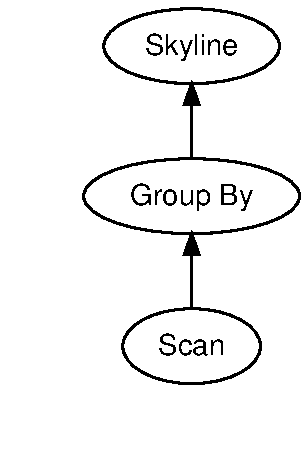
\includegraphics[scale=0.5]{plots-qp/qp-agg-skyline}\\
\caption{Query plan for query with aggregation and skyline operator}
\label{fig:qp-agg-skyline}
\end{figure}

\noindent
Again a violation of this limitation is reported with an appropriate
error message, e.g.:

\begin{interactive}
\sqlprompt{SELECT id, COUNT(*) FROM a15d1e5s0 GROUP BY id SKYLINE OF d1 MIN;}
ERROR:  column "a15d1e5s0.d1" must appear in the GROUP BY clause or be used 
in an aggregate function
\end{interactive}

%\subsection{\inlinesql{SKYLINE OF} is different to SQL:2003 \inlinesql{WINDOW} clause}

\section{PostgreSQL Architecture and Concepts}

Before we go into the details we would like to give a brief overview
of PostgreSQL architecture. According to \citep{Conway2006a} PostgreSQL
has five main components:

\begin{enumerate}
\item \emph{parser / analyzer:\/} parse the query string
\item \emph{rewriter:\/} apply rewrite rules. SQL views work by means of this mechanism.
\item \emph{optimizer:\/} determine an efficient query plan
\item \emph{executor:\/} execute a query plan
\item \emph{utility processor:\/} process DDL statements like \inlinesql{CREATE TABLE}
\end{enumerate}

\noindent
How these components work together to execute a query is illustrated
in \autoref{fig:pgsql-arch}.

\begin{figure}[htbp]
\centering
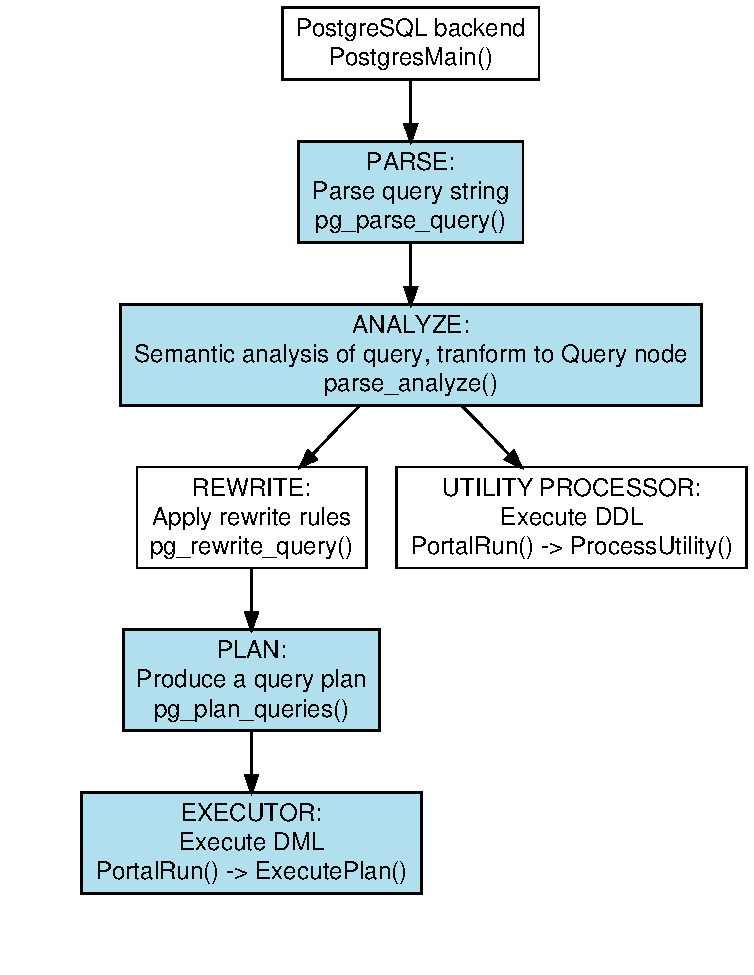
\includegraphics[scale=0.75]{plots-qp/pgsql-arch}
\caption{Architecture Diagram. Light blue background indicates the components we modified to support skyline queries.}%
\label{fig:pgsql-arch}%
\end{figure}

In the following subsections we describe some concepts of PostgreSQL
which are essential to understand our implementation.

\subsection{Pathkeys\index{pathkeys}}
\label{sec:pathkeys}
In a sole set oriented algebra there is no concept of \emph{nextness}
or \emph{order of tuples}, but in an RDBMS the relative order of
tuples is an important \emph{physical property} of a tuple stream.
The knowledge about this is encoded in PostgreSQL in terms of so
called \emph{pathkeys}, they arise naturally in conjunction with an
access path, e.g.  when scanning a tuple via a clustered index or
using an index scan.
\emph{Pathkeys} are essentially a list of \emph{pathkey}'s, where a single
pathkey encodes the sort order on a single column, actually this can
be an arbitrary expression and a pathkey contains a reference to the
according target list entry, furthermore the sort operator and a flag
on how to treat NULL values (cf. \texttt{NULLS FIRST}/\texttt{NULLS
LAST}). The information if the sort order is ascending (\texttt{ASC})
or descending (\texttt{DESC}) is encoded in the sort operator used, as
sort operator always appear in pairs, an operator and its commutator,
i.e. the same order just reversed.  This pathkeys information plays an
important role throughout the query plan.  A node within the query plan
might create, can make use of, or destroy a certain pathkeys.  If
created or preserved the nodes higher up in the query plan can make
use of it as well.  This information is considered by the query planner when
deciding among different physical operators, e.g. \emph{stream
aggregate operator} vs. \emph{hash aggregate operator}, or different
forms of the \emph{join operator}, for \emph{duplicate elimination}
and so forth. \emph{Selection}, \emph{projection} and their like
typically preserve pathkey, i.e. relative tuple order remains the
same. Others like \emph{index scan} and \emph{sort operator} establish
a certain relative order.


\subsection{Pipelined execution}
PostgreSQL query execution engine has a top down driven pipelined
architecture, i.e. each node consumes the tuples from its children and
produces tuples and in general no intermediate results are
materialized, see \srcref{src/backend/executor/README}.  A simple
suitable interface for this iterator would just expose these methods:
\texttt{open()}, \texttt{tuple next()} and \texttt{close()}.  Nevertheless
PostgreSQL's iterator interface is a bit richer, the dispatch functions
are in \srcref{src/backend/executor/execProcnode.c}. In order to specialize
just add an appropriate case in the these dispatch function and call
your own code:

\begin{lstlisting}[language=pseudo,numbers=none]
ExecCountSlotsNode -- count tuple slots needed by plan tree
ExecInitNode       -- initialize a plan node and its subplans
ExecProcNode       -- get a tuple by executing the plan node
ExecEndNode        -- shut down a plan node and its subplans
\end{lstlisting}

\noindent
Dispatch functions for less frequent used methods are in
\srcref{src/backend/executor/exexAmi.c}:

\begin{lstlisting}[language=pseudo,numbers=none]
ExecReScan               -- Reset a plan state node so that its 
                         -- output can be re-scanned
ExecMarkPos              -- Marks the current scan position
ExecRestrPos             -- restores the scan position previously
                         -- saved with ExecMarkPos
ExecSupportsBackwardScan -- does a plan type support backwards
                         -- scanning?
\end{lstlisting}

\noindent
Each execution node is coded in the fashion of a state machine.  Do
something in each state and then if necessary proceed to another
state.  The whole state is stored in the node's execution state
information and is preserved across calls.

\subsection{Simple Object System: Nodes}
\label{sec:simple-object-system}
As described in \citep[Page 12-14]{Conway2006a} PostgreSQL has a very
simple object system with the support for single inheritance.
The C structure \texttt{Node} is the root of the class hierarchy.

\pagebreak[2]

\begin{lstlisting}[language=pseudo,
caption={PostgreSQL simple object system},
label={code:simple-object-system}
]
typedef struct
{
	NodeTag type;
} Node;

typedef struct
{
	NodeTag	type;
	int		baseclass_field;
} Baseclass;

typedef struct
{
	Baseclass	baseclass;
	int			subclass_field;
} Subclass;
\end{lstlisting}

Since the memory layout for \texttt{Baseclass} and the first member of
\texttt{Subclass} (\texttt{baseclass}) is the same, a pointer \texttt{Subclass *}
can be treated like \texttt{Baseclass *}.  The first field of any class
in this simple object system is \texttt{NodeTag}, which is used to determine
a \texttt{Node}'s specific type at runtime.

There are a couple of support functions to work with the object
system: \texttt{makeNode} (create a new \texttt{Node}), \texttt{IsA}
(runtime type testing), \texttt{equal} (deep equality test),
\texttt{copyObject} (deep object copy),
\texttt{nodeToString}/\texttt{stringToNode} (serialize/deserialize
to/from text).

\noindent
When introducing new classes make sure to update these files: \\
\srcref{src/backend/nodes/\{equalfuncs,copyfuncs,outfuncs\}.c}.

\section{Parsing the \inlinesql{SKYLINE OF}-clause}
In the parser component the textual representation of a query, namely
SQL, is parsed into a data structure.  This is done as described in
the PostgreSQL documentation for the \postgresdocu{parser-stage.html}
{parser stage}.  The data structure uses PostgreSQL simple object
system, as described in the previous section.  We extended this stage
to handle the \inlinesql{SKYLINE OF}-clause as defined in
\autoref{sec:sql-extension}, see in \srcref{src/backend/parser/gram.y}
the definition of \texttt{skyline\_clause}.  The result of this
stage is called \emph{parse tree}.

\section{Query Analyzing}
In this phase, which is also described in PostgreSQL documentation on the
\postgresdocu{parser-stage.html}{parser stage}, the \emph{parse tree}
from the previous stage is semantically analyzed, the outcome is
called \emph{query tree}.  Look-ups into the system catalog are done in
this stage to resolve references to tables, columns, functions, and
operators, see \texttt{transformSkylineClause}\footnote{in
\srcref{src/backend/parser/parse\_clause.c}}.

\section{Query Rewriting}
For our implementation it was not necessary to modify the \emph{query
rewriting} stage.  For details see documentation on the
\postgresdocu{rule-system.html}{PostgreSQL Rule System}.

\section{Query Planning/Optimizing}
The \emph{query tree} from the previous stage is transformed into a
\emph{plan tree} during this stage.  Usually there are different
possible plans for a given query.  The goal is to create an optimal
plan.  Although it is computational feasible to examine each possible
plan and selecting the best, often this exhaustive enumeration is
to expensive.  
%
Various trade-offs are made, more details see PostgreSQL documentation
on \postgresdocu{planner-optimizer.html}{Planner/Optimizer}.

In the following subsections we describe how we modified the query
planner/optimizer:


\subsection{Selecting Indexes}
It is well known fact that the skyline operator is insensitive to the
order of attributes, i.e. the query

\begin{interactive}
SELECT * FROM a15d1e4s0 SKYLINE OF d1 MIN, d2 MIN;
\end{interactive}

\noindent
and

\begin{interactive}
SELECT * FROM a15d1e4s0 SKYLINE OF d2 MIN, d1 MIN;
\end{interactive}

\noindent
produce the same result.  Clearly the same is not true in general for

\begin{interactive}
SELECT * FROM a15d1e4s0 ORDER BY d1, d2;
\end{interactive}

\noindent
and

\begin{interactive}
SELECT * FROM a15d1e4s0 ORDER BY d2, d1;
\end{interactive}

\noindent
Yet alone from this example one get the intuition that the
\inlinesql{SKYLINE~OF}-clause can versatile a richer set of indexes
(access paths) than the \inlinesql{ORDER~BY}-clause.  To be
precise we must speak of \emph{pathkeys}\index{pathkeys}, i.e. both of
the above skyline queries can make use of the following index, but
only the first query with a \inlinesql{ORDER~BY}-clause:

\begin{interactive}
CREATE INDEX ix_a15d1e4s0_d1 ON a15d1e4s0 (d1, d2);
\end{interactive}

A proof for this property is given in
\autoref{sec:attributeorder}. We modified the query planner
accordingly, c.f.  function \texttt{query\_planner}\footnote{in
\srcref{src/backend/optimizer/plan/planmain.c}} and
\texttt{grouping\_planner}\footnote{in \srcref{src/backend/optimizer/plan/planner.c}}.
The matching of the pathkeys is done in \texttt{skyline\_pathkeys\_contained\_in}
\footnote{in \srcref{src/backend/optimizer/path/pathkeys.c}}.

This modification has an impact on how the join trees are formed and
which access paths are considered.

\subsubsection{Pull up subqueries}
If a subqueries contains a \inlinesql{SKYLINE~OF}-clause the query
must to be flattened out, i.e. pull up the subquery.  The function
\texttt{is\_simple\_subquery}\footnote{in
\srcref{src/backend/optimizer/prep/prepjointree.c}} as modified
accordingly.

\subsection{Preserving relative tuple order}
\label{sec:relative-tuple-order}
The relative order of tuples is an important physical property of a
tuple stream, knowledge about this is encoded in terms of
\emph{pathkeys}\index{pathkeys} as described in \autoref{sec:pathkeys}. As a
full-blown operator we have to provide this information for the skyline
operator es well.  In the \autoref{sec:bnl-tuple-order},
\ref{sec:sfs-tuple-order}, and \ref{sec:ef-tuple-order} in subsections
respectively, we bring forward arguments why BNL does \emph{not}
preserve the relative tuple order, independent from the tuple window
policy used, and that SFS and EF \emph{do} preserve the relative tuple
order.  As the two dimensional with presort algorithm is a special
case of SFS it shares the same properties.  For the one dimensional
case and for our \naive algorithms it is easy to see that they
preserve the relative tuple order.  The properties are summarized in
\autoref{tab:tuple-order-preserving}. Note that for the
\emph{established pathkeys} property we cheat a bit here, as the order
is actually established by an extra planned sort node and this is only
done when the required order is not prior established, for instance by
an index scan.

This knowledge is encoded in the function
\texttt{skyline\_method\_preserves\_tuple\_order}\footnote{in \srcref{src/backend/utils/skyline/skyline.c}} and \texttt{grouping\_planner}\footnote{in \srcref{src/backend/optimizer/plan/planner.c}}.

\begin{table}[htbp]
\centering
\begin{tabular}{lcc}
\emph{Physical Operator} & \emph{Preserves Pathkeys} & \emph{Establishes Pathkeys}\\
\hline
1DIM            & yes & no  \\
1DIM\_DISTINCT  & yes & no  \\
MNL             & yes & no  \\
2DIM\_PRESORT   & yes & yes \\
BNL             & no  & no  \\
SFS             & yes & yes \\
EF              & yes & no  \\
\end{tabular}
\caption{Tuple Order (Pathkeys) preserving / establishing Property}
\label{tab:tuple-order-preserving}
\end{table}


\subsection{Physical operator selection}
\label{sec:operatorselection}
The physical operator selection, we also call this \emph{method}, is
rather straight forward.  If a method is specified in the skyline options,
this method is taken, only some sanity checks are performed.  

In the one dimensional case either 1DIM or 1DIM\_DISTINCT is selected
depending on the usage of \inlinesql{SKYLINE OF DISTINCT}.  This
happens also if a suitable access path is present, as we do not make
use of such an access path yet.  We justify this limitation as we
believe one dimensional skyline is of limited use anyway (see
\autoref{sec:index-scan-for-1dim}).

In the presence of a suitable access path, for two dimensions
2DIM\_PRESORT and for higher dimensions SFS is selected.

BNL is the \emph{catch all} default. The physical operator selection
is implemented in the function \texttt{skyline\_choose\_method}\footnote{in
\srcref{src/backend/utils/skyline/skyline.c}}.  We acknowledge that
this behavior is hardcoded and it should be more based on cardinality
and cost estimation, here space for improvements is left, see
\autoref{sec:cardinality-and-cost-estimation}.


\subsection{Using relation statistics}
\label{sec:using-relation-statistics}
When using the tuple window placement policy \emph{entropy} a so
called \emph{entropy value} for each tuple is computed, see
\autoref{sec:tuplewindowpolicies}.
In \eqref{eqn:entropy} it as assumed that the domain for each
attribute is $[0, 1]$.  For a real world implementation this
restriction must be relaxed.  To still be able to use
\eqref{eqn:entropy} we scale the domain for each attribute to $[0,
1]$.  We use PostgreSQL statistics on the base relations to get the
information about the range of each attribute.  If at least one of
them is missing, we do fall back to placement policy \emph{append}.  In
future work we might engage \emph{sampling} here, see
\autoref{sec:sampling}.

On downside we noticed is that PostgreSQL 8.3.5 does not do a good job
with statistics and subqueries, i.e. PostgreSQL does not derive the
stats for a the subselect in, even without the
\inlinesql{LIMIT}-clause:

\begin{interactive}
SELECT * 
FROM 
    (SELECT * FROM i15d1e6s0 LIMIT 1000) AS a 
SKYLINE OF d1 MIN, d2 MIN WITH WINDOWPOLICY=ENTROPY;
\end{interactive}

\subsection{Cardinality and Cost Estimation}
\label{sec:cardinality-and-cost-estimation}
For a full-blown relational operator it is important to compute or at
least estimate the \emph{cardinality} of the result, i.e. answer the
question how many tuples will be in the output, based on the number of
tuples in the input and possible other properties of the input.  A
related question is what is the computational cost of computing the
result.  It is sufficient to answer the last question relative to
other operators.  

Unfortunately neither question is easy two answer, at least for the
non-trivial skyline algorithms like BNL and SFS it's not. Of course
the question about the cardinality is independent from the algorithms
selected.

The first bounds for the number of comparisons required have been
derived by \citet{Kung1975}, where the number of comparisons for
$n$ vectors in $d$-dimensional space is denoted by $C_d(n)$. 
Clearly $C_1(n) = n - 1$ and $C_d(n) \le O(n^2)$ for $d \ge 2$.
In their paper they showed:

\begin{eqnarray}
C_d(n) &\le& O(n \log n) \quad \textnormal{for} \quad d = 2, 3, \\
C_d(n) &\le& O(n (\log n)^{d-2}) \quad \textnormal{for} \quad d \ge 4, \quad \textnormal{and} \\
C_d(n) &\ge& \lceil\log n!\rceil \quad \textnormal{for} \quad d \ge 2
\end{eqnarray}

The first result for the cardinality was obtained by
\cite{Bentley1978}.  The result they derived is for set of $n$ vectors
in a $d$-dimensional space under the assumption that all $(n!)^d$
relative orderings are equally probable, the average number of maxima
is:

\begin{equation}
O((\ln n)^{d-1})
\end{equation}

\noindent
\citet{Buchta1989} refined this result to:

\begin{equation}
\Theta\left(\frac{(\ln n)^{d-1}}{(d-1)!}\right)
\end{equation}

\noindent
The work of \citet{Godfrey2002} elaborates this results more in the
context of skyline queries, but still under strong assumptions, like
uniform distribution and unique real-valued attributes.
%
The most recent work we are aware of about cardinality and cost
estimation for the skyline operator is the paper of
\citet{Chaudhuri2006}. A theorem for estimating the cardinality of a skyline
dataset drawn from an arbitrary distribution is derived.  This theorem is
relaxed to estimate categorical attributes as well. Cost estimation
for BNL and SFS is addressed.

In our implementation we took the result from \citet{Buchta1989} for
cardinality estimation see \texttt{estimate\_skyline\_cardinality}\footnote{in
\srcref{src/backend/optimizer/plan/createplan.c}}.

In PostgreSQL the costs are expressed in a multiple of these values:
\texttt{seq\_page\_cost}, \texttt{random\_page\_cost}, \texttt{cpu\_tuple\_cost},
\texttt{cpu\_index\_tuple\_cost}, and \texttt{cpu\_operator\_cost}
\footnote{see \srcref{src/backend/optimizer/path/costsize.c}}.

Our planner/optimizer is not yet cost-based, see
\autoref{sec:cost-based-operator-selection}, therefore we took little
effort to estimate the costs for the different physical skyline
operators, especially the results from \citet{Chaudhuri2006} have not
yet been integrated. Nevertheless a skeleton with some flesh is there,
see \texttt{cost\_skyline}\footnote{in
\srcref{src/backend/optimizer/path/costsize.c}}.

\subsubsection{Tuple window size}
One could be tempted to set the tuple window size according to the
outcome of the cardinality estimation, but the assumption that at no
time more than \texttt{output\_tuples} will be in the window does not
hold. To see this imagine the BNL algorithm running on a uniformly
distributed dataset, which implies the expected result set size is
$\Theta(\log(n)^{d-1} / (d-1)!)$ but the order of the tuple stream is
as such that before seeing the actual skyline tuples a lot of
anti-correlated tuples show up in the tuple stream.  The tuple window
will fill up with non skyline tuples.

We would like also to point out, that larger window and and less
passes do not always mean better runtime, as with larger windows the
number of comparisons per tuple could increase and therefore more CPU
time is required, so there is a break even point. 
% For experimental results see \autoref{sec:analysis-window-size}.
% NOTE: we did not analyse this data, so this section is missing

\subsubsection{\inlinesql{LIMIT} / \inlinesql{TOP $k$}}
The \inlinesql{LIMIT}/\inlinesql{TOP $k$}-clause are used to limit the
number of tuples in the result.  In the implementation no special
measures had to be taken, as the \inlinesql{LIMIT}/\inlinesql{TOP
$k$}-node will stop fetching tuple as soon as enough tuples have been
seen.  If a \inlinesql{LIMIT}/\inlinesql{TOP $k$} is present we use
this information in the cost and cardinality cost estimation.  Also
see \texttt{skyline\_method\_can\_use\_limit}\footnote{in
\srcref{src/backend/utils/skyline/skyline.c}}.

\section{Query Execution}
\label{sec:queryexecution}

The original System R prototype compiled query plans into machine
code, whereas other systems like INGRES, the grandfather of
PostgreSQL, generated an interpretable query plan. In the 1980 query
interpretation was considered a ``mistake'' by the INGRES
authors. Moore's law and enabling cross-platform portability, every
system now compiles queries into some kind of interpretable data
structure; the only difference across systems these days is the level
of abstraction \citep{Hellerstein2005}. We stick to the representation
as a tree, as it is used by PostgreSQL (see
\autoref{fig:qp-agg-bnl-sort}).

\begin{figure}[htbp]
\centering
\subfloat[Query Plan]{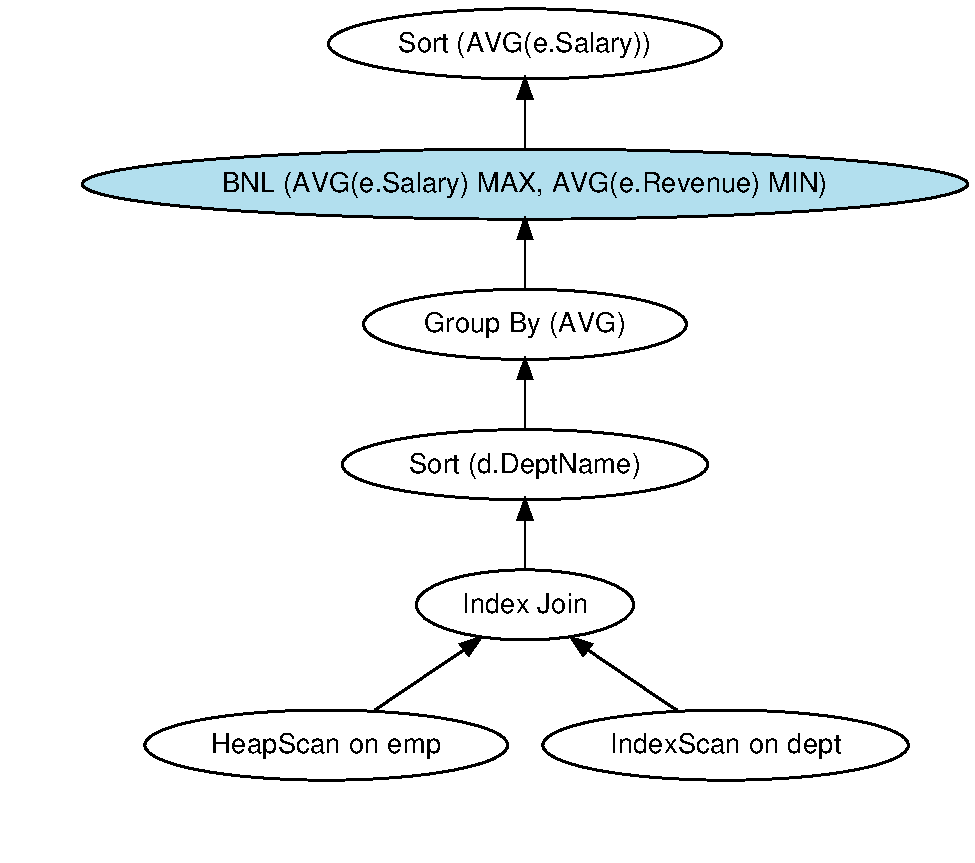
\includegraphics[scale=0.5]{plots-qp/qp-agg-bnl-sort}}\\
\subfloat[Query]{%
\parbox{100mm}{%
\texttt{%
SELECT d.DeptName, AVG(e.Salary), AVG(e.Revenue)\\
FROM emp e JOIN dept d on (e.Dno = d.DeptId)\\
GROUP BY d.DeptName\\
SKYLINE OF AVG(e.Salary) MAX, AVG(e.Revenue) MIN\\
ORDER BY AVG(e.Salary) DESC
}
}
}%
\caption{Example query plan for BNL}%
\label{fig:qp-agg-bnl-sort}%
\end{figure}

%

\begin{figure}[htbp]
\subfloat[BNL+EF]{%
\begin{minipage}[b]{\onecolumnwidth}%
\centering%
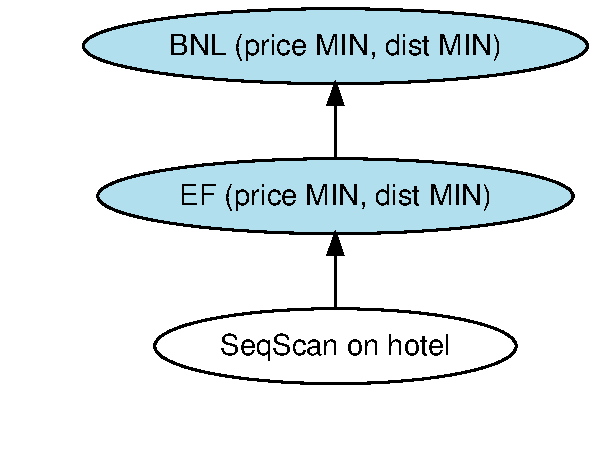
\includegraphics[scale=0.5]{plots-qp/qp-bnl-ef}%
\label{fig:qp-bnl-ef}%
\end{minipage}%
}%
\hspace{\columnsep}%
%
\subfloat[SFS+EF]{%
\begin{minipage}[b]{\onecolumnwidth}%
\centering%
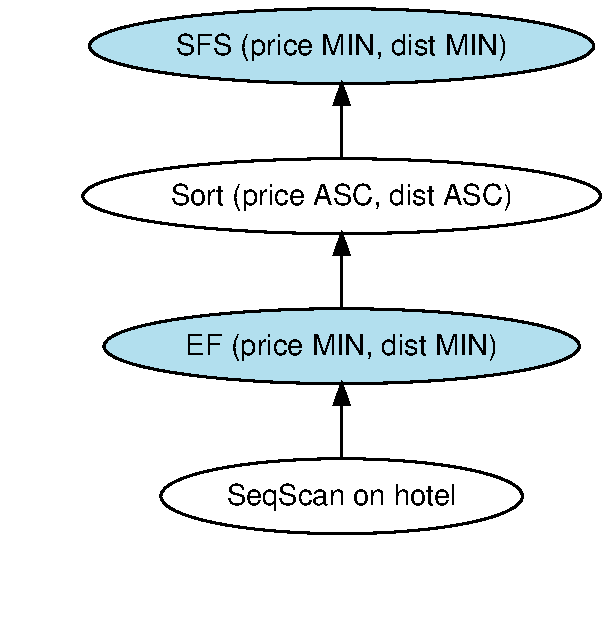
\includegraphics[scale=0.5]{plots-qp/qp-sfs-ef}%
\end{minipage}
\label{fig:qp-sfs-ef}%
}%
%
\\
%
\subfloat[SFS \emph{w/ index}]{%
\begin{minipage}[b]{\onecolumnwidth}%
\centering%
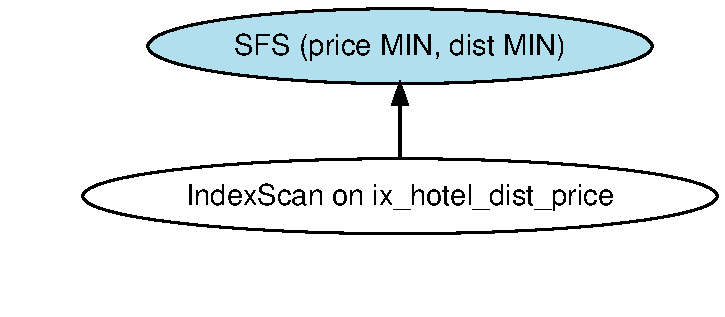
\includegraphics[scale=0.5]{plots-qp/qp-sfs-index}%
\label{fig:qp-sfs-index}%
\end{minipage}%
}%
\hspace{\columnsep}%
%
\subfloat[SFS+EF \emph{w/ index}]{%
\begin{minipage}[b]{\onecolumnwidth}%
\centering%
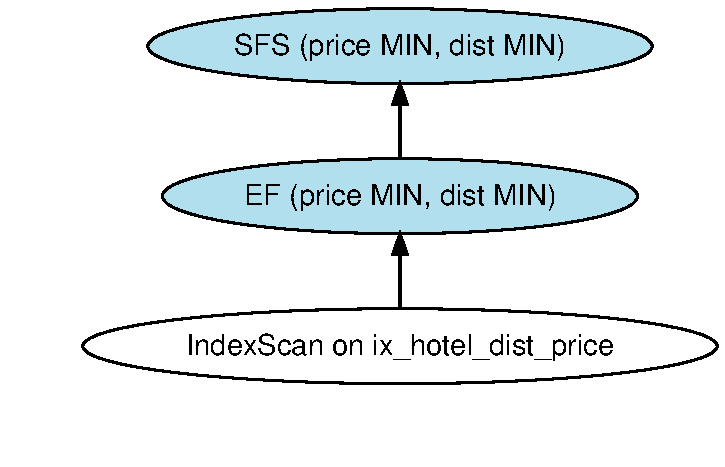
\includegraphics[scale=0.5]{plots-qp/qp-sfs-index-ef}%
\label{fig:qp-sfs-index-ef}%
\end{minipage}%
}%
\caption{Query plans for: 
\texttt{SELECT * FROM hotel SKYLINE OF price MIN, dist MIN;}}%
\end{figure}


\subsection{Comments on the Pseudo-code}
All the pseudo code presented in the following subsections is in a
form of state machines, as required for the PostgreSQL query execution
engine.  On concept that we like to mention at this point is the
\emph{tuple table}.  During query execution tuples are stored in a
tuple table when passed around between the nodes of the execution plan.
A tuple table is made up of a set of \emph{tuple table slots} or \emph{slots}
for short.  This concept is used throughout the code.


\subsection{Special case: one dimensional}
\label{sec:onedim-nondistinct}
Although this case is of limited use, the general case algorithms like
BNL and SFS can handle this case, and more over it is expressible in
SQL in a very natural way, we have a special implementation for this
case.  A skyline query of this type typically looks like:

\begin{interactive}
\textbf{SELECT * FROM a15d1e4s0 SKYLINE OF d1 MIN;}
\end{interactive}

\noindent
which rewrites to the following standard SQL query:

\begin{interactive}
\textbf{SELECT * FROM a15d1e4s0 WHERE d1 = (SELECT MIN(d1) FROM a15d1e4s0);}
\end{interactive}

\noindent
As can be seen from the query plan below the standard SQL query takes
two passes over the input, first finding the minimum by means of
aggregation and than filtering the input with the found minimum.

\begin{interactive}
                                    QUERY PLAN                                   
---------------------------------------------------------------------------------
 Seq Scan on a15d1e4s0  (cost=318.01..636.01 rows=1 width=124)
   Filter: (d1 = \ttdolar0)
   InitPlan
     ->  Aggregate  (cost=318.00..318.01 rows=1 width=8)
           ->  Seq Scan on a15d1e4s0  (cost=0.00..293.00 rows=10000 width=8)
\end{interactive}

\noindent
Another way to express this query in standard SQL is:

\begin{interactive}
\textbf{SELECT * FROM a15d1e4s0 o WHERE NOT EXISTS
    (SELECT * FROM a15d1e4s0 i WHERE i.d1 < o.d1);}
\end{interactive}

\noindent
but this is even worse, and has a runtime complexity of $O(n^2)$, this
approach corresponds to a \naive nested-loop, the query plan is
accordingly:

\begin{interactive}
                                    QUERY PLAN                                   
---------------------------------------------------------------------------------
 Seq Scan on a15d1e4s0 o  (cost=0.00..1247.10 rows=5000 width=4)
   Filter: (NOT (subplan))
   SubPlan
     ->  Seq Scan on a15d1e4s0 i  (cost=0.00..318.00 rows=3333 width=124)
           Filter: (d1 < \ttdolar0)
\end{interactive}

We took a different approach, while scanning over the input we collect
all minimal tuples in a tuple store\index{tuple store}.  For
comparison we need to keep just one tuple.  If a tuple is equal to
this, i.e. another potential minimal/maximal tuple we add it to the
tuple store.  On the other hand, if this tuple is dominated we clean
the tuple store, and keep the dominating tuple.  After the initial
scan over the input we pipe out the tuple store,
cf. \autoref{code:1dim}.  For the sake of a clearer pseudo-code we
gave our self the freedom to present the tuple store interface
(\texttt{tuplestore\_*}) a little different to the actual
implementation.  A functionality we added to the tuple store is to
remove all tuples from the tuple store, which is cheaper than
recreating it.  In the pseudo-code this function is called
\texttt{tuplestore\_clearall}, while in the real implementation its name
is \texttt{tuplestore\_catchup}, which fits better as we are just
modifying read and write pointers.

%\begin{figure}[htbp]
\begin{lstlisting}[language=pseudo,
caption={Pseudo-code for Special case: 1 dimensional},
label={code:1dim}
]
function ExecSkyline_1Dim(var $state$)
	switch $state.status$
	case INIT:
		tuplestore_init($state.tuplestore$);

		$resultSlot \gets$ ExecProcNode(outerPlanState($state$));

		if $resultSlot \not=$ NULL
			// input contains at least one tuple
			$slot \gets$ ExecProcNode(outerPlanState($state$));

			// while not end of input reached
			while $slot \not=$ NULL
				if $slot \nondistinct resultSlot$
					// we found another potential minimal tuple
					tuplestore_put($state.tuplestore$, $slot$);
				else if $slot \dominates resultSlot$
					// we found a new lower bound
					$resultSlot \gets slot$;
					tuplestore_clearall($state.tuplestore$);
					tuplestore_put($state.tuplestore$, $slot$);

				$slot \gets$ ExecProcNode(outerPlanState($state$));

		$state.status \gets$ PIPEOUT;

		// fall through

	case PIPEOUT:
		if $\neg$tuplestore_eof($state.tuplestore$)
			return tuplestore_get($state.tuplestore$);
		else
			tuplestore_done($state.tuplestore$);
			$state.status \gets$ DONE;
			return NULL;

	case DONE:
		return NULL;
\end{lstlisting}
%\caption{Pseudo-code for Special case: 1 dimensional}
%\label{code:1dim}
%\end{figure}

\subsection{Special case: one dimensional with distinct}
\label{sec:onedim-distinct}
Again this case is of limited use and all general skyline algorithms
can deal with it, we implemented a specialized algorithm for this
case.  It is even simpler than the non-distinct case and it easy to
see that a single scan over to input while keeping the current
minimal/maximal tuple suffices to compute the skyline in this case,
one just has to take care of border cases, such as no tuples in the
input, see \autoref{code:1dimdistinct}. A skyline query of this type looks
like:

\begin{interactive}
\textbf{SELECT * FROM a15d1e4s0 SKYLINE OF DISTINCT d1 MIN;}
\end{interactive}

\noindent
and will return at most one tuple, if more than one minimal tuple
exists our implementation returns the first.

The SQL:2003 Standard \citep{SQL2003} does not provide a way
to limit the size of a result set. Nevertheless PostgreSQL and other
RDBMS do provide syntax for this and consider it during query
planning. The query and the query plan for the above query in without
the skyline operator would look like:

\begin{interactive}
\textbf{SELECT * FROM a15d1e4s0 WHERE d1 = (SELECT MIN(d1) FROM a15d1e4s0) LIMIT 1;}
\comment{output omitted}

\textbf{EXPLAIN SELECT * FROM a15d1e4s0 WHERE d1 = }\ellipsis

                                    QUERY PLAN                                   
---------------------------------------------------------------------------------
 Limit  (cost=318.01..636.01 rows=1 width=124)
   InitPlan
     ->  Aggregate  (cost=318.00..318.01 rows=1 width=8)
           ->  Seq Scan on a15d1e4s0  (cost=0.00..293.00 rows=10000 width=8)
   ->  Seq Scan on a15d1e4s0  (cost=0.00..318.00 rows=1 width=124)
         Filter: (d1 = \ttdolar0)
\end{interactive}

\noindent
Please note that again two scans over the input are done, although the
second might stop earlier. For Microsoft SQL Server to same query
would look like this:

\begin{interactive}
\textbf{SELECT TOP 1 * FROM a15d1e4s0 WHERE d1 = (SELECT MIN(d1) FROM a15d1e4s0);}
\end{interactive}

\noindent
An ad hoc experiment that we conducted showed that Microsoft SQL Server
2005 produces a very similar execution plan.

In Oracle the pseudo-column \inlinesql{ROWNUM}\index{ROWNUM@\texttt{ROWNUM}}
can be used the limit the number of tuples returned by a query.

If the relation in question contains a unique identifier with a total
order, let us call it \texttt{id}, then the following solution in
standard SQL can be found:

\begin{interactive}
\textbf{SELECT * FROM a15d1e4s0 o WHERE NOT EXISTS
    (SELECT * FROM a15d1e4s0 i WHERE i.d1 < o.d1 OR (i.d1 = o.d1 AND i.id < o.id));}
\end{interactive}

\noindent
Note that condition \texttt{i.d1 = o.d1 AND i.id < o.id} is used to
select the first, according to the order induced by \texttt{id}, of the
minimal tuples. The runtime complexity of this query is also in $O(n^2)$.

%\begin{figure}[htbp]
\begin{lstlisting}[language=pseudo,
caption={Pseudo-code for Special case: 1 dimensional distinct},
label={code:1dimdistinct}
]
function ExecSkyline_1DimDistinct(var $state$)
	switch $state.status$
	case INIT:
		$resultSlot \gets$ ExecProcNode(outerPlanState($state$));

		if $resultSlot \not=$ NULL
			$slot \gets$ ExecProcNode(outerPlanState($state$));

			// while not end of input reached
			while $slot \not=$ NULL
				if $slot \dominates resultSlot$
					$resultSlot \gets slot$;

				$slot \gets$ ExecProcNode(outerPlanState($state$));

		$state.status \gets$ DONE;
		return $resultSlot$;

	case DONE:
		return NULL;
\end{lstlisting}
%\caption{Pseudo-code for Special case: 1 dimensional distinct}
%\label{code:1dimdistinct}
%\end{figure}


\subsection{Special case: two dimensional with presort}
\label{sec:presort}
The two dimensional case of skyline computation is usually the
smallest case considered in literature and of course BNL and SFS can
deal with it.  Nevertheless as pointed out in \citep{Borzsonyi2001}
skylines for the two dimensional case can be computed in a simple way
if the input relation is ordered according to the skyline criteria,
then the skyline can be computed with a single scan over the
input, while keeping just the most recently found skyline tuple, see
\autoref{code:2dimpresort}.  Of course in the presents of an
suitable access path the input need not to be sorted, just perform an
index scan.  This method is simple to implement, and we believe the
two dimensional case is already a quite useful one, from a users
perspective.

An interesting aspect of this algorithm is how it deals with the
\inlinesql{DISTINCT} modifier for the \inlinesql{SKYLINE~OF}-clause.
%
For the semantics of the \inlinesql{DISTINCT}-modifier see
\autoref{sec:rewrite-queries-with-distinct}.
%
In the pseudo-code in \autoref{code:2dimpresort} \texttt{DISTINCT}
is a Boolean variable, which is \emph{true} if the
\inlinesql{DISTINCT} modifier is present, and \emph{false}
otherwise. Let $p$ be the current skyline tuple, then a tuple $q$
becomes the next skyline if the following condition holds:

\begin{equation}\label{eqn:2dimpf}
q \dominates p \lor (q \nondistinct p \land \text{\texttt{DISTINCT}}).
\end{equation}

\noindent
If \texttt{DISTINCT} is \emph{true}, then \eqref{eqn:2dimpf} simplifies to:

\begin{eqnarray}
q \dominates p \lor (q \nondistinct p \land \top) &=& q \dominates p \lor q \nondistinct p \nonumber\\
&\stackrel{\textnormal{by \eqref{eqn:weakdominats-dom-nondistinct}}}{=}& q \weakdominates p
\end{eqnarray}

\noindent
Otherwise if \texttt{DISTINCT} is \emph{false}:
%
\begin{equation}
q \dominates p \lor (q \nondistinct p \land \bot) = q \dominates p
\end{equation}

\pagebreak[4]
%\begin{figure}[htbp]
\begin{lstlisting}[language=pseudo,
caption={Pseudo-code for Special case: 2 dimensional with presort},
label={code:2dimpresort}
]
function ExecSkyline_2DimPresort(var $state$)
	switch $state.status$
        case INIT:
		$resultSlot \gets$ ExecProcNode(outerPlanState($state$));

		if $resultSlot\ =$ NULL
			// input does not contain a single tuple
			$state.status \gets$ DONE;
			return NULL;

		$state.status \gets$ PROCESS
		// the first tuple is already a skyline tuple
		return $resultSlot$;

	case PROCESS:
		forever
			$slot \gets$ ExecProcNode(outerPlanState($state$));

			if $slot\ =$ NULL
				// end of input reached
				$state.status \gets$ DONE;
				return NULL;

			if $slot \dominates returnSlot \lor (slot \nondistinct returnSlot\ \land$ DISTINCT$)$
				// found another skyline tuple
				$returnSlot \gets slot$;
				return $returnSlot$;

	case DONE:
		return NULL;
\end{lstlisting}
%\caption{Pseudo-code for Special case: 2 dimensional with presort}
%\label{code:2dimpresort}
%\end{figure}

\subsection{\Naive method: \emph{MNL: materialized nested loop}}
\label{sec:mnl}
This method is the first general method which can deal with any
dimensionality and treat the \inlinesql{DISTINCT} modifier.  In
directly corresponds to the \naive $O(n^2)$ nested loop approach,
compare every tuple to all others as long no witness is found, which
dominates the current tuple.  Why is it called \emph{materialized}
nested loop?  This \emph{materialized} stem from the fact that we
materialize the tuples from the outer plan, to be able to read them
over and over again, this is because the skyline operator can sit at
any non leave node in the query plan and not only on top of a table or
index scan.  To handle the \inlinesql{DISTINCT} case, we just use a
the counters $state.pos$ and $innerPos$ and favor the first tuple.

%\begin{figure}[htbp]
\begin{lstlisting}[language=pseudo,
caption={Pseudo-code for MNL},
label={code:mnl}
]
function ExecSkyline_MaterializedNestedLoop(var $state$)
	switch $state.status$
	case INIT:
		ExecMarkPos(outerPlanState($state$));
		$state.pos \gets 0$;
		$state.status \gets$ PROCESS

		// fall through

	case PROCESS:
		forever
			// get next current tuple
			ExecRestrPos(outerPlanState($state$));
			$slot \gets$ ExecProcNode(outerPlanState($state$));
			$state.pos \gets state.pos + 1$;
			ExecMarkPos(outerPlanState($state$));

			if $slot\ =$ NULL
				// end of input reached
				$state.status \gets$ DONE;
				return NULL;

			// dominance check
			ExecReScan(outerPlanState($state$));

			$innerPos \gets 0$;

			forever
				$innerSlot \gets$ ExecProcNode(outerPlanState($state$));
				$innerPos \gets innerPos + 1$;

				if $innerSlot\ =$ NULL
					// no witness found
					return $slot$;

				if $innerSlot \dominates slot$
					break;
				else if $innerSlot \nondistinct slot \land$ DISTINCT
					// favor the first
					if $innerPos < state.pos$
						break;
		break;

	case DONE:
		return NULL;
\end{lstlisting}
%\caption{Pseudo-code for MNL}
%\label{code:mnl}
%\end{figure}

\subsection{Tuple Window}
A tuple window is a data structure used by BNL, SFS and EF to store
skyline (candidate) points. As internal representation we used a double
linked list with a sentinel (cf. \citep[Page 204--209]{Cormen2001}).
Using a sentinel simplifies the code to manipulate a double linked
list a lot.

The external interface is simple iterator interface with a few more
functions\footnote{see \srcref{src/include/utils/tuplewindow.h}}:

\begin{itemize}
\item \lstinline|TupleWindowState *tuplewindow_begin(int maxKBytes, int maxSlots, TupleWindowPolicy policy)|
creates a tuple window with the maximum size of \lstinline|maxKBytes|
KB or if a a maximum of \lstinline|maxSlots| slots. The number of
slots is the stronger limit. For policy see
\autoref{sec:tuplewindowpolicies}.  The returned value must be
used in all subsequent calls to the tuple window interface functions.

\item \lstinline|void tuplewindow_end(TupleWindowState *state)| 
destroys a tuple window and frees all resources.

\item \lstinline|void tuplewindow_clean(TupleWindowState *state)|
removes all tuples from the tuple window.

\item \lstinline|bool tuplewindow_has_freespace(TupleWindowState *state)|
returns true of the tuple window can hold at least one more tuple.
Note that we are ignore the fact that the tuple that is going to be
inserted might consume a little more space than is actually left, but
this eases the implementation and an existing PostgreSQL interface the
\lstinline|tuplestore| interface is designed in the same way.

\item \lstinline|void tuplewindow_setinsertrank(TupleWindowState *state, double rank)|
when policy \emph{entropy} or \emph{ranked} is used, the rank of the
new tuple has to be set with this function before starting to scan
over the tuple window, so ensure to call
\lstinline|tuplewindow_rewind| prior to this call.

\item \lstinline|void tuplewindow_puttupleslot(TupleWindowState *state, TupleTableSlot *slot, int64 timestamp, bool forced)|
insert the tuple in the tuple table slot \lstinline|slot| into the
tuple window with the given timestamp.  For a ranked window policy
\lstinline|forced| can be set to true, i.e. if the new tuple has a
higher rank than the lowest ranked tuple in the window that this
lowest ranked tuple is removed, if the space for the higher ranked
tuple is needed.  We use this especially for the implementation of the
elimination filter. We speak of a \emph{forced insert}\index{forced
insert}.  Currently the \lstinline|timestamp| argument is only used
by BNL all other algorithms set it to zero.

\item \lstinline|void tuplewindow_rewind(TupleWindowState *state)|
set the \emph{cursor} to the first tuple.

\item \lstinline|bool tuplewindow_ateof(TupleWindowState *state)|
return true of cursor is at the end of the tuple window.

\item \lstinline|void tuplewindow_movenext(TupleWindowState *state)|
move the cursor to the next tuple.

\item \lstinline|void tuplewindow_removecurrent(TupleWindowState *state)|
remove the current tuple.  Note that this also modifies the cursor.
So when calling \lstinline|tuplewindow_removecurrent|, calling
\lstinline|tuplewindow_movenext| afterwards skips over a tuple.

\item \lstinline|bool tuplewindow_gettupleslot(TupleWindowState *state, TupleTableSlot *slot, bool removeit)|
get the tuple a the current position of the cursor.  When called with
\lstinline|removeit| true, the returned tuple is removed from the
tuple window.  Note that this is not the same as calling
\lstinline|tuplewindow_gettupleslot| and
\lstinline|tuplewindow_removecurrent|, as
\lstinline|tuplewindow_removecurrent| also frees the tuple it self and
not only removing it from the tuple window.

\item \lstinline|int64 tuplewindow_timestampcurrent(TupleWindowState *state)|
returns the timestamp of the tuple at cursor position.  Currently only
used by BNL.

\end{itemize}



\subsubsection{Placement Policies}
\label{sec:tuplewindowpolicies}
With tuple window placement policy we want to express how tuples are
organized in the window and in which order the are compared against
each other \citep{Godfrey2007}. The implementation supports four
different placement policies:
\begin{enumerate}
\item \emph{append:} 
a new tuple is always inserted at the \emph{end} of the list

\item \emph{prepend:}
instead at the end, new tuples are inserted at the \emph{beginning} of
the list

\item \emph{entropy:}
tuples are keep in \emph{rank descending order}. The inserted position
is found in $O(n)$, this is done by computing the rank before starting
to scan over the window and the pointer is only incremented as long as
the rank of the tuple to be inserted is smaller or equal to the rank
of the current tuple. We choose this approach because the tuple window
is scanned anyway. With this policy and a \emph{forced insert}, in
case the tuple window is full, the tuple with the lowest ranking is
removed from the window to make space for a higher ranked tuple.

Let $r$ be a tuple and $r_1, \ldots, r_m$ the attributes the skyline
is computed on with $\forall i \in \{1, \ldots, m\}\colon: r_i \in [0,
1]$, then the entropy value $E(r)$ for the tuple $r$ is defined as
(see \citep{Chomicki2003,Chomicki2005}):

\begin{equation}\label{eqn:entropy}
E(t) = \sum_{i=1}^{m} \ln(r_m + 1)
\end{equation}

\item \emph{random: }
behalves like \emph{entropy} but instead of a an computed entropy value
for a tuple a random value is used

\end{enumerate}

\subsection{BNL}
The implementation of the BNL algorithm is based on our fixed version
of \citep{Borzsonyi2001}, see \autoref{code:fixedbnl}. In the
following we give a pseudo-code in terms of a state machine as
required by the PostgreSQL query execution engine, see
\autoref{code:fixedbnl-statemachine}. This implementation is fully general, it can deal with any dimension $\ge 1$ and can treat the \inlinesql{DISTINCT} modifier. To ensure BNL is used for query execution specify the \inlinesql{BNL}
keyword as an option to the skyline clause.  All other options that
can be specified effect the tuple window.


%\begin{figure}[htbp]
\begin{lstlisting}[language=pseudo,
caption={Pseudo-code for BNL},
label={code:fixedbnl-statemachine}
]
function ExecSkyline_BlockNestedLoop(var $state$)
	forever
		switch $state.status$
		case INIT: 
			$state.source \gets$ OUTER; 
			tuplestore_init($state.tempOut$);
			tuplewindow_init($state.window$);
			$state.tsIn \gets 0$; 
			$state.tsOut \gets 0$; 
			$state.status \gets$ PROCESS; 
			break;

		case PROCESS:
			if $state.source$ = OUTER
				$slot \gets$ ExecProcNode(outerPlanState($state$));
			else
				$slot \gets$ tuplestore_get($state.tempIn$);

			if $slot =$ NULL
				if $state.source$ = TEMP
					tuplestore_done($state.tempIn$);

				if $state.tsOut = 0$
					// nothing written to temp -> done
					tuplestore_done($state.tempOut$);
					tuplewindow_rewind($state.window$);
					$state.status \gets$ FINALPIPEOUT;
					break;

				$state.source \gets$ TEMP;
				$state.tempIn \gets state.tempOut$;
				tuplestore_init($state.tempOut$);
				$state.tsIn \gets 0$;
				$state.tsOut \gets 0$;
				tuplewindow_rewind($state.window$);
				$state.status \gets$ PIPEOUT;
				break;

			$state.tsIn \gets state.tsIn + 1$;

			tuplewindow_rewind($state.window$);
			if $state.ranked$
				tuplewindow_setinsertrank($state.window$, ExecSkylineRank($state$, $slot$);

			forever
				if tuplewindow_ateof($state.window$)
					if tuplewindow_hasfreespace($state.window$)
						tuplewindow_put($state.window$, $slot$);
					else
						tuplestore_put($state.tempOut$, $slot$);
						$state.tsOut \gets state.tsOut$;

					break;

				$innerSlot \gets$ tuplewindow_current($state.window$);

				if $innerSlot \dominates slot \lor (innerSlot \nondistinct slot \land \text{DISTINCT})$
					break;
				else if $slot \dominates innerSlot$
					tuplewindow_removecurrent($state.window$);
				else
					tuplewindow_movenext($state.window$);

			tuplewindow_rewind($state.window$);
			$state.status \gets$ PIPEOUT;
			break;

		case PIPEOUT:
			while $\neg$tuplewindow_ateof($state.window$)
				if tuplewindow_timestampcurrent($state.window$) = $state.tsIn$
					return tuplewindow_get($state.window$);
				
				tuplewindow_movenext($state.window$);

			$state.status \gets$ PROCESS;
			break;

		case FINALPIPEOUT:
			if $\neg$tuplewindow_ateof($state.window$)
				return tuplewindow_get($state.window$);

			tuplewindow_done($state.window$);
			$state.status \gets$ DONE;
			return NULL;

		case DONE:
			return NULL;
\end{lstlisting}
%\caption{Pseudo-code for BNL}
%\label{code:fixedbnl-statemachine}
%\end{figure}

% fake caption
%\begingroup
%\makeatletter
%\def \@captype {figure}%
%\makeatother
%\caption{lala}
%\endgroup

\subsection{SFS}
\autoref{code:sfs} translates straight forward into a state machine,
the way it fits into the query execution engine, see
\autoref{code:sfs-statemachine}.

\begin{lstlisting}[language=pseudo,
caption={Pseudo-code for SFS},
label={code:sfs-statemachine}
]
function ExecSkyline_SortFilterSkyline(var $state$)
	forever
		switch $state.status$
		case INIT: 
			$state.source \gets$ OUTER; 
			tuplestore_init($state.tempOut$);
			tuplewindow_init($state.window$);
			$state.neednextrun \gets false$;
			$state.status \gets$ PROCESS; 
			break;

		case PROCESS:
			if $state.source$ = OUTER
				$slot \gets$ ExecProcNode(outerPlanState($state$));
			else
				$slot \gets$ tuplestore_get($state.tempIn$);

			if $slot =$ NULL
				if $state.source$ = TEMP
					tuplestore_done($state.tempIn$);

				if $\neg state.neednextrun$
					// nothing written to temp -> done
					tuplestore_done($state.tempOut$);
					tuplewindow_rewind($state.window$);
					$state.status \gets$ DONE;
					return NULL;

				$state.source \gets$ TEMP;
				$state.tempIn \gets state.tempOut$;
				tuplestore_init($state.tempOut$);
				tuplewindow_clean($state.window$);
				$state.neednextrun \gets false$;
				break;

			tuplewindow_rewind($state.window$);
			if $state.ranked$
				tuplewindow_setinsertrank($state.window$, ExecSkylineRank($state$, $slot$);

			forever
				if tuplewindow_ateof($state.window$)
					if tuplewindow_hasfreespace($state.window$)
						tuplewindow_put($state.window$, $slot$);
						return $slot$;
					else
						tuplestore_put($state.tempOut$, $slot$);
						$state.neednextrun \gets true$;

					break;

				$innerSlot \gets$ tuplewindow_current($state.window$);

				if $innerSlot \dominates slot \lor (innerSlot \nondistinct slot \land \text{DISTINCT})$
					break;

				tuplewindow_movenext($state.window$);
			break;

		case DONE:
			return NULL;
\end{lstlisting}

\subsection{Elimination Filter (EF)}
The pseudo-code is already given in \autoref{sec:ef-tuple-order},
cf. \autoref{code:ef}. We have used the elimination filter with
SFS and BNL, see the following sections.

\subsection{SFS+EF (a LESS Variant)}
In \citep{Godfrey2005} \nospellcheck{Godfrey et al.} proposed the LESS
algorithm, which is an improvement of SFS due to the introduction of
the concept of {\em elimination filter} (EF). With the original LESS
algorithm the elimination filtering is carried out in the pass zero of
the external sort routine to eliminate records quickly.

In our case, in order to integrate the elimination filter into the SFS
algorithm, while at the same time preserving the utilization of the
physical sort operator, we implemented the elimination filter {\em
before} the sort routine.  Speaking in terms of the iterator tree, the
EF node is a child of the sort node, which in turn is a child of the
SFS node (see \autoref{fig:qp-sfs-ef}).  Furthermore, we do not
integrate the skyline computation into the final pass of the merge
sort phase, as described in \citep{Godfrey2005}.  Therefore,
technically speaking, SFS+EF is not an equivalent implementation of
LESS.  However, the elimination filter is preserved in SFS+EF, which
is essentially the gist of LESS.

The implementation of EF is similar to BNL.  An elimination filter
window is maintained in the main memory.  We use 8~KB as default
window size.  The difference between EF and BNL is that EF does not
write tuples to a temporary file if the tuple window is full, and that
the relative order of tuples going through the EF is preserved.



\subsection{BNL+EF}
Inspired from the idea of the elimination filter in LESS, we
experimented a new combination of BNL and EF. That is, the elimination
filter is executed before the BNL algorithm. Since our implementation
of the elimination filter is independent from the external sort
routine, the coding of this variant is straightforward.  It turns out
that the algorithm BNL+EF is a substantial improvement to BNL.



\section{Development}
In this section we would share some of the experience we have made 
during development.

\subsection{Source Code and Version Control}
We started out our implementation effort of the skyline operator, when
\texttt{CVS HEAD} of the PostgreSQL source repository was
\texttt{8.3-devel}, i.e. the version 8.3 of PostgreSQL was currently
under development.  PostgreSQL's source is kept in a Concurrent Versions
System (CVS) repository.  We have used the very handy
\href{http://www.tortoisecvs.org/}{Tortoise CVS} to checkout and
update the PostgreSQL source.  We keep our source in a
\href{http://subversion.tigris.org/}{SubVersion} (SVN) repository, and use
\href{http://tortoisesvn.tigris.org/}{TortoiseSVN} to interact with our
repository.

For each CVS tag we are interested in, namely \texttt{CVS HEAD} and
\texttt{REL8\_3\_STABLE}, we keep the entire source tree as a branch 
in our SVN repository, including the CVS metadata directories
\texttt{CVS}.  By means of that we continuously merged \texttt{CVS HEAD}
into our main development branch, called \texttt{trunk} in the
SubVersion terminology.  In order to have a more stable and
reproducibly setting we decided to base this paper on the branch
\texttt{REL8\_3\_STABLE}, i.e. all experiments in this paper are based
on Version 8.3.0 of PostgreSQL with our patch for the skyline
operator applied.

Having the entire CVS source tree in the SVN repository is handy, it
was quite easy to merge in the changes from \texttt{CVS HEAD} into
\texttt{trunk}.  To support this task we wrote two scripts, as CVS
detects changes based on the file modification date/time, where SVN
really looks at the file content.

\begin{itemize}
\item \texttt{cvs-entries-normalize.sh:}
sorts the content of the \texttt{CVS/Entries*} files, to have a
normalized form, and minimize the changes that are committed to the
SVN repository.

\item \texttt{resetcvsts.pl:}
sets the file date/time according to the values in \texttt{CVS/Entries},
this allows to easily move around the working copy across different machines.
\end{itemize}

Another benefit of using SVN was the smooth integration with an
issue/bug-tracker called \href{http://trac.edgewall.org/}{Trac}.  Trac
has a wiki, milestones, all kinds of reports and that like, and
proved itself as very handy for this size and type of project.

\subsection{Debugging PostgreSQL}
PostgreSQL creates one back-end process, which corresponds to an
operating system process, per client connect.  This property makes
debugging a bit unpleasant.  Nevertheless there is a good work around
for this, just operate the PostgreSQL in \emph{single user
mode}\index{single user mode}.  This gives one a prompt, to enter
queries directly and the query is evaluated in the same process.  So
debugging or with Microsoft Visual C++ even \emph{edit \&
continue}\index{edit \& continue}\footnote{Edit \& continue is the
ability of modifying the source code while debugging, apply the changes
and continue to debug.  Kind of deluxe for a C compiler.}.  For further
details see PostgreSQL documentation on
\postgresdocu{app-postgres.html}{postgres}

\subsection{Regression Testing}
To facilitate regression testing we also integrated a test case in
PostgreSQL regression test suite.  This test case tests just a few
very basic scenarios, as a throughout test would take quite some time,
and this would not be appreciated as part of a checked build.  For the
basic regression test see
\srcref{src/test/regress/sql/skyline\_base.sql} and
\srcref{src/test/regress/expected/skyline\_base.out}.

For a more extensive test see the Perl script \texttt{slregress.pl},
here a larger set of test cases is produced and the result is always
checked against the query expressed in standard SQL.  Instead of a
table the random dataset returning function as described in
\autoref{sec:set-returning-function} is used.

We ran both, the PostgreSQL regression test suite and our Perl script
\texttt{slregress.pl}, regularly during development, to ensure that
we did not break other parts of PostgreSQL and an already implemented
feature of the skyline operator, while we were integrating new parts
or optimize and/or refactor other parts.




%%
%% CHAPTER: Results
%%



\chapter{Results}
\label{chap:results}


\section{Experimental Setup}
We ran our experiments on seven Dell OptiPlex 755, Intel Pentium
Dual-Core CPU E2160 (1.80GHz, 1MB L2 cache), with 1~GB RAM and Seagate
Barracuda 160~GB HDD (7200~rpm, SATA 3.0Gb/s, 8~MB cache) with a
single NTFS partition,
% average latency 4.16msec
running Microsoft Windows XP (SP2).
% 
Our implementation was based on PostgreSQL 8.3.0 and was compiled
using Microsoft Visual Studio 2005 (SP1) using the \texttt{RELEASE}
configuration with assertions disabled.
%
PostgreSQL was configured to use 200 MB of RAM for shared buffers,
with auto vacuuming disabled, and all other settings were left as
default.

If not otherwise mentioned, a tuple window size of 1024~KB (equal to
the PostgreSQL \texttt{work\_mem} setting), and an EF tuple window
size of 8~KB (equal to the PostgreSQL block size) were used.

The tables for the test runs have been generated using the extended
version \citep{Eder2007a} of the dataset generated presented in
\citep{Borzsonyi2001}, which allows to generate tables with
different initial seeds for the random generator. All experiments
were carried out on three different sets with varying initial seed, for each
distribution type (independent, correlated, and anti-correlated), and
with 100, 500, 1k, 5k, 10k, 50k, 100k tuples.

Each tuple consists of a unique 4 byte integer \emph{id} and 15
randomly generated 8 byte floats $d_1, \ldots, d_{15}$. With a 23 byte
tuple header and the alignment it sums up to a tuple length of 152 bytes. 
The memory chunk used by the PostgreSQL memory allocation function
(\texttt{palloc}) was 264 bytes long.
%The tuples are 152 bytes long, but the memory chunk used by PostgreSQL memory allocation function (palloc) is 264 bytes long.
%
%23 bytes tuple header, (0 bytes for null value bitmap) 
%
%data align at 8:
%4 (id) + 8 * 15 (d1-d15) = 124
%
%= 148 + alignment = 152
%
%MAXALIGN 
%MAXIMUM_ALIGNOF 8
%
%http://www.postgresql.org/docs/current/static/storage-page-layout.html

For the experiments using an index, a duplicate of the same set of
tables was used, including six indexes, where index $k$ is an index on
$d_1, \ldots, d_k$.  This all sums up to 126 tables and an database of
approximately 1 GB.  For most of our experiments we did not consider
tables with more than 100k tuples, as the runtime for a 15 dimensional
skyline query on 100k tuples went up to 30 minutes. Consult
\autoref{sec:totalworkload} for the total computational workload
done in the experiments.

% TODO hot cache, we ensure the table is in the shared buffer, before
% running the query, as each of the implemented methods has to read the
% entire table anyway

All experiments were carried out with a \emph{hot disk cache},
i.e. due to appropriate queries all pages were in the shared
buffers. See \autoref{sec:experimentalenvironment} for more
details.


\subsection{Lesson learned}
\label{sec:lessonlearned}
A lesson we have painfully learned during our experiments is to
minimize all possible influences on the runs to avoid skewed
results. This especially includes: screen savers, power saving or
standby options and any form of automatic software update such as
Microsoft Windows Update or Google Pack software updater.

\subsection{Random Dataset Generator}

For our experiments we used a modified version \citep{Eder2007a} of
the popular dataset generator from \citep{Borzsonyi2001}.  Our
modified version can be used as command line utility or as a
PostgreSQL module. The PostgreSQL module provides a set returning
function and creates datasets on the fly.  The details are described
in the following sections.  But first of all we describe which type of
dataset are generated by the dataset generator.

\subsubsection{Independent, Correlated, and Anti-Correlated Datasets}
\label{sec:corr-anti-indep}

The main parameters one can vary for a generated dataset are
\emph{cardinality}, i.e. number of tuples, \emph{dimensionality} and
the \emph{distribution type} and types are as of \citep{Borzsonyi2001}: 
\emph{independent}, \emph{correlated}, and \emph{anti-correlated}.

%Instead of giving a lenghty description of how the differnt
%distributions are generated, we present the essential parts of the
%source, as we believe this is the precisest way to describe it. Here
%are the some basic building blocks:

Before we give a detailed description of this distribution types, we
show some of the basic build blocks used for generating them, as we
believe the source code of the implementation is the precisest way to
describe it:

\begin{lstlisting}
static double
random_equal(double min, double max)
{
	double x = (double) rand() / RAND_MAX;
	return x * (max - min) + min;
}
\end{lstlisting}

As expected \lstinline{random_equal()} will return a random value $x
\in [\textnormal{min}, \textnormal{max}]$.

\begin{lstlisting}
static double
random_peak(double min, double max, int dim)
{
	int		d;
	double	sum = 0.0;

	for (d = 0; d < dim; d++)
		sum += random_equal(0, 1);
	sum /= dim;
	return sum * (max - min) + min;
}
\end{lstlisting}

The function \lstinline{random_peak()} returns a random value $x \in
[\textnormal{min}, \textnormal{max}]$ as sum of $\textnormal{dim}$
equally distributed random values.

\begin{lstlisting}
static double
random_normal(double med, double var)
{
	return random_peak(med - var, med + var, 12);
}
\end{lstlisting}

This function \lstinline{random_normal()} is our way to generate a
normally distributed value $x \in (\textnormal{med} -
\textnormal{var}, \textnormal{med} + \textnormal{var})$ with expected
value $E[x] = \textnormal{med}$.
%
This implementation is motivated through the central limit theorem and
based on the observation that a $12$-fold sum of $[0,1]$ uniformly
distributed random value yields a sufficient good normally distributed
value. A pre-requirement for this to work, is that the $12$ uniformly
distributed values are independent. While this can not be guaranteed
for \lstinline{random_equal()} we verified that data generated by
\lstinline{random_normal()} are sufficiently normally distributed with
the Shapiro-Wilk test.

\pagebreak[4]

Now we focus on the different distribution types and how they are
generated and we show some of their properties:

\begin{itemize}
\item \emph{indep}: 
for this type of dataset, all attribute values are generated
independently using a uniform distribution. 
\autoref{fig:density-2d-i2d1e5} shows an density plot
and statistics of such an independent dataset with 100k tuples and $d
= 2$. The skyline tuples of this dataset are the lower left corners of
the red line, where the red line is the ``skyline''. The density of
points within a specific subregion is indicated by grayscale values,
the darker the more points are in the subregion. Above and to the
right of the grayscale density plot is the border distribution for
each dimension, in this plots the blue line indicates the density of a
normal distribution with the same mean and standard deviation as the
border distribution.

The implementation is as straight forward as expected:

\begin{lstlisting}
int		d;

for (d = 0; d < dim; d++)
	x[d] = random_equal(0, 1);
\end{lstlisting}

\begin{figure}[htbp]
\centering
\sbox{\tempbox}{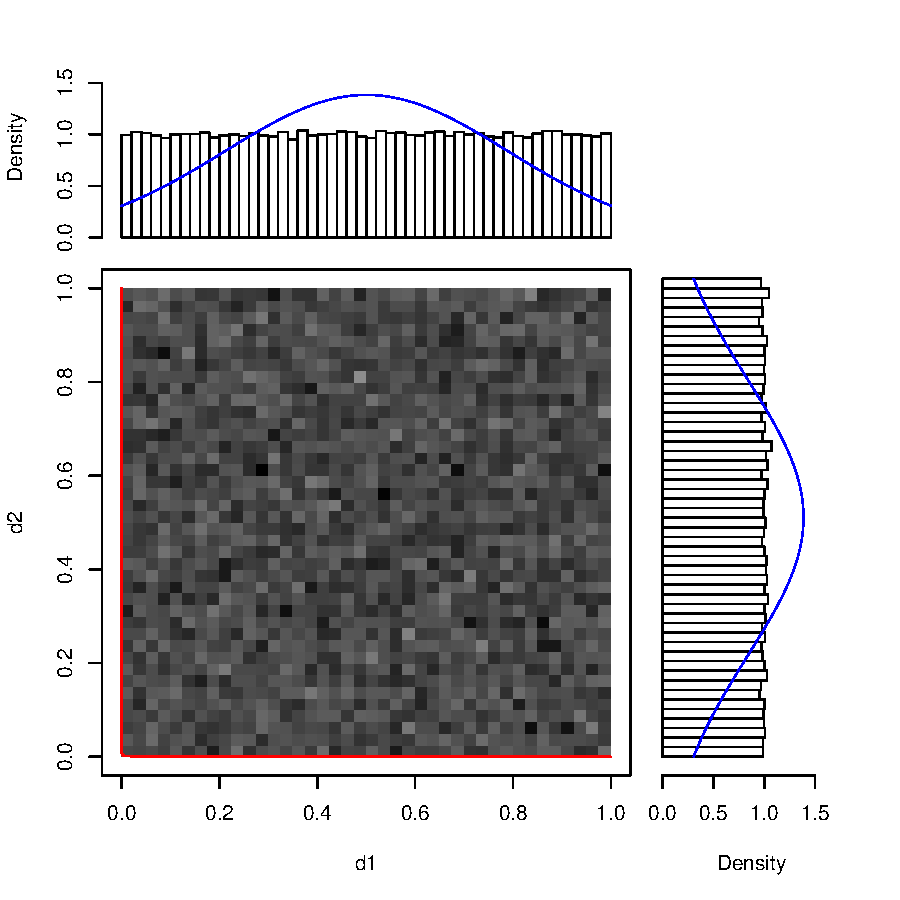
\includegraphics[width=100mm]{plots-density/density-2d-i2d1e5}}%
\subfloat[Density Plot]{\usebox{\tempbox}}%
\subfloat[Statistics]{%
\begin{minipage}[b]{38mm}%
\vbox to \ht\tempbox{%
\vfil
\begin{tabular}[b]{r|rr}%
	& d1 	& d2 \\
\hline
mean	& 0.500 & 0.500 \\
var	& 0.083 & 0.083 \\
\hline
cor	& d1	& d2 \\
\hline
d1	& 1.000 & 0.000 \\
d2	& 0.000 & 1.000 \\
\end{tabular}%
\vfil
}
\end{minipage}%
}%
\caption{Independent dataset (100k tuples)}%
\label{fig:density-2d-i2d1e5}%
\end{figure}

\pagebreak[4]

\item \emph{corr}: 
a correlated dataset represents an environment in which points which
are good in one dimension are also good in the other dimensions. 

%For instance, students which have a good publication record typically also
%do well in their preliminaries. 

A vector $x$ with the dimension $dim$ is generated in the following way:

\begin{lstlisting}
do
{
	int		d;
	double	v = random_peak(0, 1, dim);
	double	l = v <= 0.5 ? v : 1.0 - v;
	
	for (d = 0; d < dim; d++)
		x[d] = v;

	for (d = 0; d < dim; d++)
	{
		double h = random_normal(0, l);
		x[d] += h;
		x[(d + 1) % dim] -= h;
	}
} while (!is_vector_ok(dim, x));
\end{lstlisting}

Due to the way it is computed an $x[d]$ could get out of the bound,
\lstinline{is_vector_ok()} verifies that all coordinates of $x$ are
within the interval $[0,1]$.

\autoref{fig:density-2d-c2d1e5} shows a correlated dataset with
100k tuples for $d = 2$.

\begin{figure}[htbp]
\centering
\sbox{\tempbox}{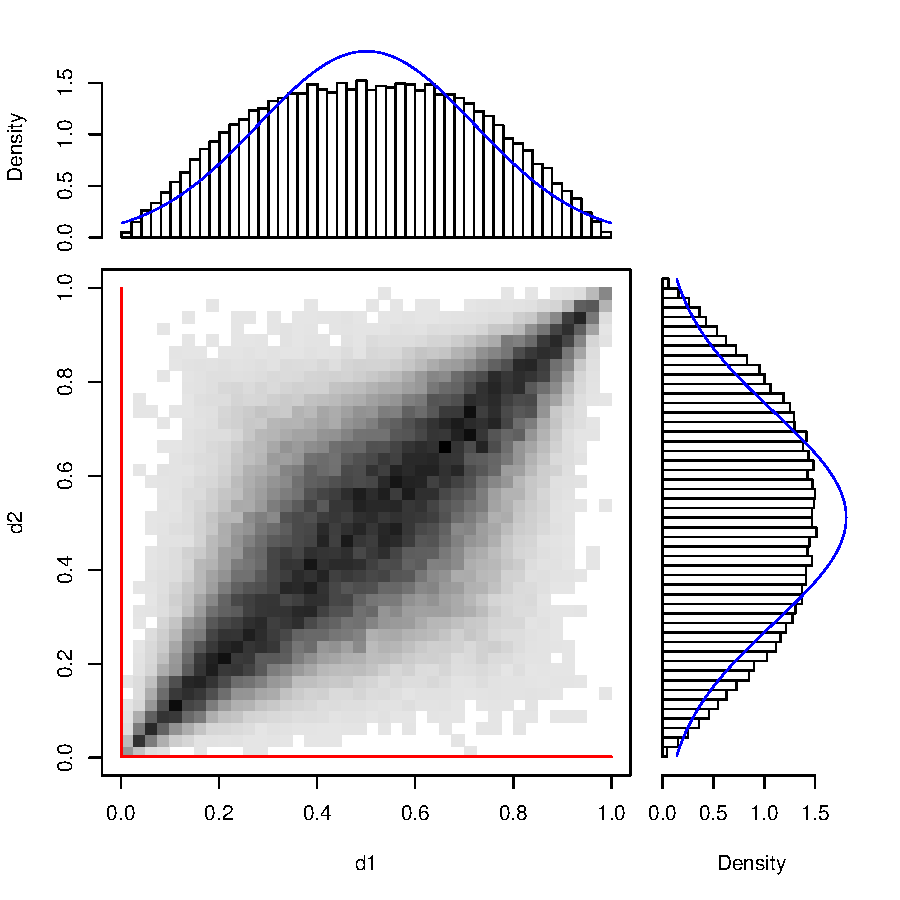
\includegraphics[width=100mm]{plots-density/density-2d-c2d1e5}}%
\subfloat[Density plot]{\usebox{\tempbox}}%
\subfloat[Statistics]{%
\begin{minipage}[b]{38mm}%
\vbox to \ht\tempbox{%
\vfil
\begin{tabular}[b]{r|rr}
	& d1 	& d2 \\
\hline
mean	& 0.500 & 0.500 \\
var	& 0.049 & 0.049 \\
\hline
cor	& d1	& d2 \\
\hline
d1	& 1.000 & 0.717 \\
d2	& 0.717 & 1.000 \\
\end{tabular}
\vfil
}
\end{minipage}
}
\caption{Correlated dataset (100k tuples)}%
\label{fig:density-2d-c2d1e5}%
\end{figure}

\pagebreak[3]

\item \emph{anti}:
an anti-correlated dataset represents an environment in which points
which are good in one dimension are bad in one or all of the other
dimensions. The standard example used in the skyline literature falls
into this category: hotels are either cheap and far away from the
beach or expensive and close to the beach.

\begin{lstlisting}
do
{
	int		d;
	double	v = random_normal(0.5, 0.25);
	double	l = v <= 0.5 ? v : 1.0 - v;
			
	for (d = 0; d < dim; d++)
		x[d] = v;
		
	for (d = 0; d < dim; d++)
	{
		double h = random_equal(-l, l);
		x[d] += h;
		x[(d + 1) % dim] -= h;
	}
} while (!is_vector_ok(dim, x));
\end{lstlisting}

\autoref{fig:density-2d-a2d1e5} shows an anti-correlated dataset
with 100k tuples for $d = 2$.
\end{itemize}

\begin{figure}[htbp]
\centering
\sbox{\tempbox}{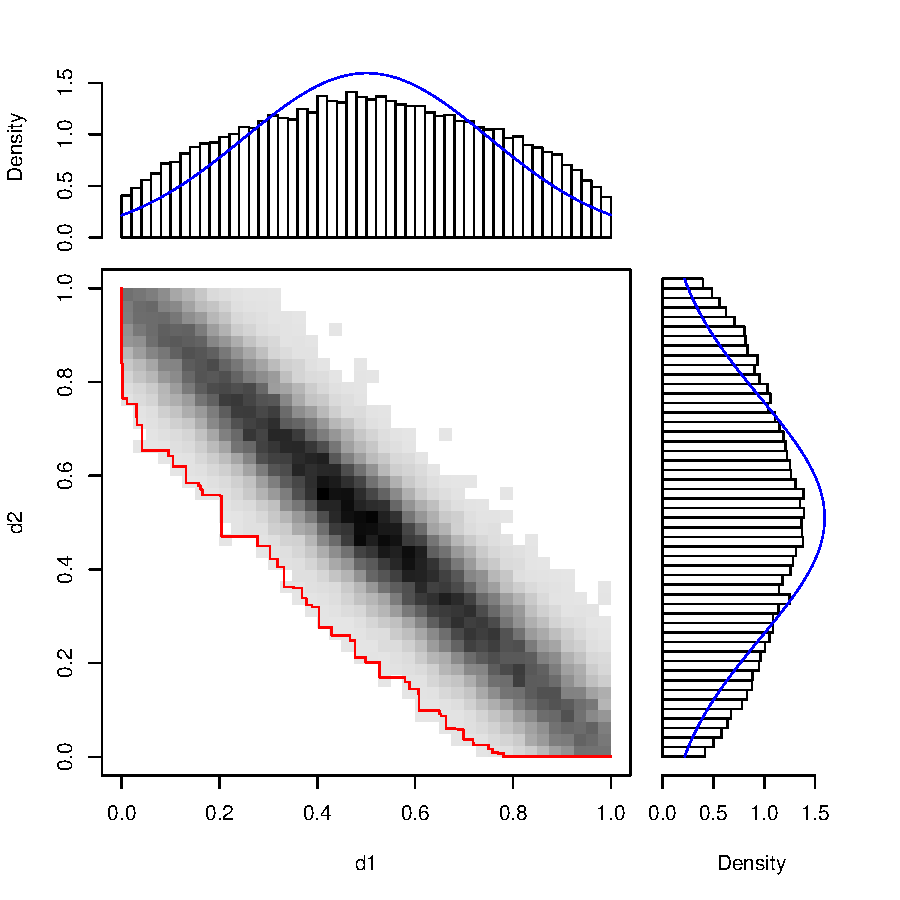
\includegraphics[width=100mm]{plots-density/density-2d-a2d1e5}}%
\subfloat[Density Plot]{\usebox{\tempbox}}%
\subfloat[Statistics]{%
\begin{minipage}[b]{38mm}%
\vbox to \ht\tempbox{%
\vfil
\begin{tabular}[b]{r|rr}
	& d1 	& d2 \\
\hline
mean	& 0.500 & 0.500 \\
var	& 0.063 & 0.063 \\
\hline
cor	& d1	& d2 \\
\hline
d1	& 1.000 & -0.944 \\
d2	& -0.9444 & 1.000 \\
\end{tabular}
\vfil
}
\end{minipage}
}
\caption{Anti-correlated dataset (100k tuples)}%
\label{fig:density-2d-a2d1e5}%
\end{figure}

For the very details of the random dataset generator, please have a
look at the implementation which is available from \citep{Eder2007a}.

\subsubsection{As command line utility}

The most beneficial use case for the command line version of the
random dataset generator is to pipe its output directly into the
database. The usage message explains how to use the command line
utility:

\begin{interactive}
\shprompt{randdataset -?}
Test Data Generator for Skyline Operator Evaluation
Usage: randdataset (-i|-c|-a) -d DIM -n COUNT [-s SEED] [-p] [-S] [-h|-?]

Options:
       -i       independent (dim >= 1)
       -c       correlated (dim >= 2)
       -a       anti-correlated (dim >= 2)

       -d DIM   dimensions >=1
       -n COUNT number of vectors
       -I       unique id for every vector
       -p PAD   add a padding field, PAD characters long

       -C       generate SQL COPY statement
       -R       generate SQL CREATE TABLE statement
       -T NAME  use NAME instead of default table name

       -s SEED  set random generator seed to SEED

       -S       output stats to stderr

       -h -?    display this help message and exit

Examples:
       randdataset -i -d 3 -n 10 -I -R
       randdataset -a -d 2 -n 100 -S
\end{interactive}

An invocation of \texttt{randdataset} suitable to pipe it directly
into \texttt{psql}, i.e. load it into database, could look like:

\begin{interactive}
\shprompt{randdataset -i -d 3 -n 10 -I -R}
DROP TABLE IF EXISTS "i3d10";
CREATE TABLE "i3d10" (id int, d1 float, d2 float, d3 float);
COPY "i3d10" (id, d1, d2, d3) FROM STDIN DELIMITERS ',' CSV QUOTE '''';
1,0.000000000000000e+00,6.900010321708401e-01,5.054183972559023e-01
2,5.914905399975788e-01,5.547849133400177e-01,3.784288188342139e-01
\ellipsis\rcomment{7 rows omitted}
10,8.585111004572880e-01,9.898449857671955e-02,8.770675234855467e-01
\ttbackslash.
\end{interactive}

\subsubsection{PostgreSQL Random Dataset Generator Function}
\label{sec:set-returning-function}

To be able to generate test datasets on the fly, i.e. with out
explicitly creating tables and filling them up, we create a PostgreSQL
module which implements the functionality of \texttt{randdataset} as a
set returning function. To create, backup and restore a test database
with an appropriate set of test tables can be very time
consuming. Having such a function at hand is useful in many situations,
all it takes is run PostgreSQL's \texttt{initdb} and install the set
returning function. We did so many times when merging PostgreSQL
8.3-devel branch into our branch, which often made it necessary to
re-\texttt{initdb}. Especially for regression tests and during
debugging this function was very handy. PostgreSQL's concept of
\postgresdocu{functions-srf.html}{set returning functions} allows to
issue queries as such:

\begin{interactive}
\sqlprompt{SELECT * FROM generate_series(2,4);}
 generate_series
-----------------
               2
               3
               4
(3 rows)
\end{interactive}

This concept of set returning functions is quite flexible and allows
also to return complex data types such as records. To test drive this
PostgreSQL 'contrib' module (see
\srcref(contrib/randdataset)), without installing it, even with
installing PostgreSQL visit our web-interface at
\url{http://skyline.dbai.tuwien.ac.at/}. To install it onto your
PostgreSQL installation follow the instructions
\srcref{contrib/randdataset/README.randdataset}. Once installed the
function can be used as follows:

\begin{interactive}
\sqlprompt{SELECT rds.id, rds.d1, rds.d2 FROM}\rcomment{columns are referred by name}
\sqlpromptcont{pg_rand_dataset('indep', 2, 10, 0) AS}\rcomment{2 dim independent dataset with 10 tuples}
\sqlpromptcont{rds(id int, d1 float, d2 float);}\rcomment{define names and types}
 id |         d1         |         d2
----+--------------------+--------------------
  1 |  0.170828036112165 |  0.749901980510867
  2 | 0.0963716553972902 |  0.870465227342427
\ellipsis\rcomment{7 rows omitted}
 10 |  0.715538595204958 | 0.0830042460388524
(10 rows)

\sqlprompt{SELECT rds.* FROM}
\sqlpromptcont{pg_rand_dataset('corr', 3, 10, 0) AS}\rcomment{3 dim, correlated, 10 tuples}
\sqlpromptcont{rds(id int, d1 float, d2 float, d3 float);}
 id |        d1         |        d2         |        d3
----+-------------------+-------------------+-------------------
  1 | 0.482522432069401 | 0.327330244422693 | 0.207248995528228
  2 | 0.448836206689892 | 0.512027726159258 | 0.600054676092416
\ellipsis\rcomment{7 rows omitted}
 10 | 0.319189108559988 | 0.407713612758059 |  0.30165467053249
(10 rows)

\sqlprompt{SELECT rds.* FROM}
\sqlpromptcont{pg_rand_dataset('anti', 3, 20, 1) AS}\rcomment{3 dim, anti-correlated, 20 tuples, seed 1}
\sqlpromptcont{rds(id int, d1 float, d2 float, d3 float);}
\comment{output omitted, as it is similar to above, except other distribution, more tuples, and another initial seed is used}
\end{interactive}

\noindent
The general signature for \inlinesql{pg\_rand\_dataset} is:
\begin{interactive}
FUNCTION pg_rand_dataset(disttype text, dim int, rows int, seed int)
RETURNS setof record
\end{interactive}

\noindent
Where the arguments have following meaning:
\begin{itemize}
\item \texttt{disttype} 
specifies the distribution type (see \autoref{sec:corr-anti-indep}),
allowed values are \texttt{'indep'}, \texttt{'corr'}, and
\texttt{'anti'}

\item \texttt{dim} specifies the number of dimensions, allowed values are 1 up to 20 

\item \texttt{rows} specifies the number of tuples that should be returned, and 

\item \texttt{seed} is the seed for the random generator
\end{itemize}

We ensured that calling \inlinesql{pg\_rand\_dataset} with the same
arguments will always return the same result set. In the PostgreSQL
terminology this property of a function is called \texttt{IMMUTABLE}
(see PostgreSQL documentation on
\postgresdocu{xfunc-volatility.html}{Function Volatility Categories}).

To make the usage more comfortable we defined a set of wrapper
functions \texttt{rds$k$d} for the dimensions $k \in \{1, \ldots,
20\}$, they allowed us to issue the same queries as above in the
following way (see \srcref{contrib/randdataset/randdataset.sql.in}):

\begin{interactive}
\sqlprompt{SELECT rds.* FROM rds2d('indep', 10, 0) AS rds;}
\ellipsis\rcomment{output completely omitted, as it is the same as above}

\sqlprompt{SELECT rds.* FROM rds3d('corr', 10, 0) AS rds;}
\ellipsis\rcomment{same here}

\sqlprompt{SELECT rds.* FROM rds3d('anti', 20, 0) AS rds;}
\ellipsis\rcomment{same here}
\end{interactive}


\subsubsection{Buffer for Set returning function}

In the PostgreSQL execution engine a function scan node is responsible
for retrieving tuples from a set returning function. The current
implementation reads all the tuples from the set returning function
and stores them in a \texttt{tuplestore} before returning the first
tuple to the caller. A \texttt{tuplestore} maintains an in memory
buffer once it runs out of memory the remaining tuples are written to
a tempfile. The size of the in memory buffer is controlled through the
configuration variable \texttt{work\_mem}. The default value is
1024~KB. This configuration variable is also used to determine the amount
of RAM used for sort operations, for merge joins, hash joins and many more.
So RAM used for a single complex query can by multiple times the value of 
\texttt{work\_mem}.
In our setting we use the configuration variable \texttt{work\_mem}
for the sort operation in SFS and as the default tuple window size for
skyline algorithms that require a tuple window. In the following query
PostgreSQL calls \texttt{generate\_series} a million times and will
discard all tuples except one due to the
\texttt{LIMIT 1}-clause.

\begin{interactive}
\sqlprompt{SELECT * FROM generate_series(1,1000000) LIMIT 1;}
 generate_series
-----------------
               1
(1 row)
\end{interactive}

This behavior is not desirable, at least we want that the tuples do
not get swapped out to disk as
\texttt{tuplestore}'s-\texttt{work\_mem} gets full, since for parts
of our experiments we were not willing to pay I/O penalty as we were
studying just the CPU bounded behavior of the skyline algorithms.

On the other hand we do not want to increase \texttt{work\_mem}, as
this would as mentioned above influence the sort operation and the size
of the tuple window for the skyline algorithms. Therefore we decided
to introduce a new configuration variable
\texttt{function\_scan\_work\_mem}, solely for the \texttt{tuplestore}
in the function scan node. The following utility query sets this
configuration variable to 100~MB;

\begin{interactive}
\sqlprompt{SET function_scan_work_mem  = 102400;}
\end{interactive}

\noindent
A patch for this feature can be found at
\srcref{patches/function\_scan\_work\_mem.diff}.


\section{Experimental Environment}
\label{sec:experimentalenvironment}
We believe the systems environment in which we carried out our
experiments is interesting on its own and therefore we sketch it in
this section.
%
First of all we would like to give some definitions of terms we use to
describe the experimental environment and how the relate to each
other. To distinguish these terms from the general terms with the same
name we start them with an upper case letter, i.e. Job vs. job.

\begin{definition}[Query]
A Query corresponds to a single SQL query with meta data embedded in
comments.
\end{definition}

\noindent
To embed meta data we are using the fact that ``\texttt{--}'' starts a
single line comment in SQL, by means of that we can safely pass any
extra information through SQL processor \texttt{psql} to the post
processing steps. In our case to the programs that parse and analyze
the log files. We use only the following types of meta data (see
\autoref{fig:jobfile}, \ref{fig:logfile}
and~\ref{fig:parsedlogfile}):

\begin{itemize}
\item 
\texttt{--<pid pid=}\textit{pid}\texttt{/>}; \textit{pid} identifies
the machine the Job ran on.

\item 
\texttt{--<comment>} and \texttt{--</comment>}; a Setup Query, see
next definition. Query between these tags are of course executed, but
in a later stage just commented out.

\item 
\texttt{--<query runid=}\textit{runid}\texttt{>} and
\texttt{--</query>}; A Run cf. definition below.  Please note that the
corresponding Setup Queries are not nested within the Run they just
precede the Run.

\item 
\texttt{--<queryplan>} and \texttt{--</queryplan>}; is used in a
later stage to preserve the query plan in the comment, but its not
used otherwise.
\end{itemize}

In our experimental studies our focus is on the execution
plan\footnote{We use execution plan and query plan interchangeable.}
and the actual run times and not on the output of a query. The output
of a query was of interest for us, when we did regression testing to
ensure our implementation is correct. To accomplish this we prefixed
our queries with \inlinesql{EXPLAIN ANALYZE}. \inlinesql{EXPLAIN}
alone just shows the execution plan of a statement without actually
running it, while \inlinesql{EXPLAIN ANALYZE} carries out the command
and shows the actual run times. See PostgreSQL documentation on
\postgresdocu{sql-explain.html}{EXPLAIN} for more details.

\begin{definition}[Setup Query]
A Setup Query is a query who's sole purpose is to setup things up for
the query that is going to be profiled.
\end{definition}

\noindent
We issued these types of query to prim the cache. Setup queries
typically look like this:

\begin{interactive}
EXPLAIN ANALYZE SELECT * FROM a15d1e5s0;
\end{interactive}

\noindent
or with an index

\begin{interactive}
EXPLAIN ANALYZE SELECT * FROM a15d1e5s0idx ORDER BY d1, d2;
\end{interactive}

\noindent
and given enough shared buffers the entire relation and the used index
will be in the disk cache afterwards. As we set the shared buffer size
why larger than our biggest relation we the associated indexes this
was always the case.

\begin{definition}[Run]
A Run comprises zero, one or more Setup Queries and the Query that is
going to be profiled.
\end{definition}

\noindent
Each Run is identified by unique \texttt{runid} and besides this
general definition in our case a Run had zero or one Setup Query and
we often grouped runs in such a way, that two runs share a single
Setup Query (cf. \autoref{fig:jobfile}).

\begin{definition}[Job]
A Job comprises of one or more Runs batched together in a file.
\end{definition}

\noindent
A Job is the smallest unit subject to workload distribution (see
\autoref{sec:jobscheduling}) and is stored in a \texttt{.sql} file
and typically looks like displayed in \autoref{fig:jobfile}.

\begin{figure}[htbp]
\begin{interactive}
--<comment>\rcomment{the setup query}
explain analyze select * from a15d1e5s0;
--</comment>
--<query runid=bnl.ef.entropy.entropy.a15d1e5s0.5>\rcomment{first run}
explain analyze select * from a15d1e5s0 \prebreak
  \postbreak skyline of d1 min, d2 min, d3 min, d4 min, d5 min \prebreak
  \postbreak with bnl windowpolicy=entropy ef efwindowpolicy=entropy;
--</query>
--<query runid=sfs.ef.entropy.entropy.a15d1e5s0.5>\rcomment{second run}
explain analyze select * from a15d1e5s0 \prebreak
  \postbreak skyline of d1 min, d2 min, d3 min, d4 min, d5 min \prebreak
  \postbreak with sfs windowpolicy=entropy ef efwindowpolicy=entropy;
--</query>
\end{interactive}
\caption{A snipped from a job file, containing a setup query and two runs}
\label{fig:jobfile}
\end{figure}


%%%      1         2         3         4         5         6         7        8
%%% 567890123456789012345678901234567890123456789012345687901234567890123456790

\begin{figure}[htbp]
\begin{interactive}
--<pid pid=SKY07/>\rcomment{the pid identifies the machine the job ran on}
--<comment>
explain analyze select * from a15d1e5s0;
                                    QUERY PLAN                                   
---------------------------------------------------------------------------------
 Seq Scan on a15d1e5s0  (cost=0.00..2924.00 rows=100000 width=124) \prebreak
   \postbreak (actual time=0.010..48.112 rows=100000 loops=1)
 Total runtime: 79.093 ms
(2 rows)

--</comment>
--<query runid=bnl.ef.entropy.entropy.a15d1e5s0.5>
explain analyze select * from a15d1e5s0 \prebreak
  \postbreak skyline of d1 min, d2 min, d3 min, d4 min, d5 min
  \postbreak with bnl windowpolicy=entropy ef efwindowpolicy=entropy;
                                    QUERY PLAN                                   
---------------------------------------------------------------------------------
 Skyline  (cost=457884.24..457886.07 rows=79 width=124) \prebreak
   \postbreak (actual time=10618.204..11076.301 rows=4550 loops=1)
... \rcomment{we skip this query plan here as the one below is more representative}
--</query>
--<query runid=sfs.ef.entropy.entropy.a15d1e5s0.5>
explain analyze select * from a15d1e5s0 \prebreak
  \postbreak skyline of d1 min, d2 min, d3 min, d4 min, d5 min \prebreak
  \postbreak with sfs windowpolicy=entropy ef efwindowpolicy=entropy;
                                    QUERY PLAN
---------------------------------------------------------------------------------
 Skyline  (cost=458169.07..458170.90 rows=79 width=124) \prebreak
   \postbreak (actual time=672.662..5747.821 rows=4550 loops=1)
   Skyline Attr: d1, d2, d3, d4, d5
   Skyline Method: sfs 5 dim
   Skyline Stats: passes=2 rows=27223, 1599
   Skyline Window: size=1024k policy=entropy
   Skyline Cmps: tuples=15109830 fields=37876691
   ->  Sort  (cost=457807.96..457809.79 rows=732 width=124) \prebreak
         \postbreak (actual time=672.653..712.584 rows=27223 loops=1)
         Sort Key: d1, d2, d3, d4, d5
         Sort Method:  external merge  Disk: 3816kB
         ->  Elimination Filter  (cost=457523.13..457773.13 rows=732 width=124) \prebreak
               \postbreak (actual time=0.014..597.068 rows=27223 loops=1)
               Elim Filter Attr: d1, d2, d3, d4, d5
               Elim Filter Method: elimfilter 5 dim
               Elim Filter Stats: passes=1 rows=
               Elim Filter Window: size=8k policy=entropy
               Elim Filter Cmps: tuples=1263179 fields=3533862
               ->  Seq Scan on a15d1e5s0  (cost=0.00..2924.00 rows=100000 \prebreak
                     \postbreak width=124) (actual time=0.009..43.352 rows=100000 loops=1)
 Total runtime: 5750.614 ms
(17 rows)

--</query>
\end{interactive}
\caption{An example for a raw log file}
\label{fig:logfile}
\end{figure}

\begin{figure}[htbp]
\begin{interactive}
\comment{All input is preserved as comment, where comment lines start with ``#''.\commentskip}
#--<pid pid=SKY07/>\rcomment{the pid identifies the machine the job ran on}
#--<comment>
#explain analyze select * from a15d1e5s0;
# \ellipsis\rcomment{the query plan is as in Figure \ref{fig:logfile}}
#--</comment>
#--<query runid=bnl.ef.entropy.entropy.a15d1e5s0.5>\commentskip
\comment{For the query sections all relevant information from the query plan is parsed into CSV format with the columns \texttt{runid}, \texttt{name} and \texttt{value}.  See \autoref{tab:queryplanfields} for a description of the name/value pairs.\commentskip{}}
"bnl.ef.entropy.entropy.a15d1e5s0.5","method","bnl.ef.entropy.entropy"
\ellipsis
"bnl.ef.entropy.entropy.a15d1e5s0.5","skyline.rows","4550"
"bnl.ef.entropy.entropy.a15d1e5s0.5","skyline.passes","2"
"bnl.ef.entropy.entropy.a15d1e5s0.5","skyline.passes.rows","27223, 1396"
\ellipsis\commentskip
\comment{Please note that the query and query plan are preserved below the data in CSV format.\commentskip{}}
#<queryplan>
#explain analyze select * from a15d1e5s0 skyline of d1 min, d2 min, \ellipsis
#                                    QUERY PLAN
#--------------------------------------------------------------------------------
# Skyline  (cost=457884.24..457886.07 rows=79 width=124)
# \ellipsis\rcomment{the query plan is as in Figure \ref{fig:logfile}}
#</queryplan>
#--</query>
#--<query runid=sfs.ef.entropy.entropy.a15d1e5s0.5>
"sfs.ef.entropy.entropy.a15d1e5s0.5","method","sfs.ef.entropy.entropy"
"sfs.ef.entropy.entropy.a15d1e5s0.5","skyline.est.cost","458169.07..458170.90"
"sfs.ef.entropy.entropy.a15d1e5s0.5","skyline.est.cost.start","458169.07"
\ellipsis\rcomment{similar for the second run}
#<queryplan>
# \ellipsis\rcomment{as above, original query plan is preserved as comment}
#</queryplan>
#--</query>
\end{interactive}
\caption{A log file parsed with \texttt{qp2log}.  For the name and description of the extracted fields see \autoref{tab:queryplanfields}.}
\label{fig:parsedlogfile}
\end{figure}

\subsection{Machine and Network Configuration}
In our experimental environment we had one machine (SKY00) to control
and monitor the experiments and seven machines (SKY01, $\ldots$,
SKY07), but this seven is just because of we did not have more.
%
To have exactly the same configuration, we cloned SKY02, $\ldots$, SKY07 from
SKY01 using a fine piece of free software namely PING (Partimage Is
Not Ghost)\footnote{available at: \url{http://ping.windowsdream.com/}}.
We also used Windows XP's \texttt{sysprep} during the clone process.

For interprocess communication we used file sharing and we used file
locking for synchronization. The machine SKY00 shared a folder, which
was mounted by SKY01, $\ldots$, SKY07 with a directory layout is
described in \autoref{tab:dirlayoutexpiriments}.

\newdimen\fixedcolumnwidth
\newdimen\paragraphcolumnwidth
\global\fixedcolumnwidth 2.2cm
\global\paragraphcolumnwidth\textwidth
\advance\paragraphcolumnwidth -\fixedcolumnwidth

\begin{table}[!ht]
\centering
\begin{tabular*}{\textwidth}{@{\extracolsep{\fill}}p{\fixedcolumnwidth}@{\extracolsep{\fill}}p{\paragraphcolumnwidth}}
\verb|jobs/|      &  \\
\verb|  js.pl|    & job scheduler, see \autoref{sec:jobscheduling} \\
\verb|  feed.pl|  & batch feeder, moves prepared jobs into the
                    \texttt{jobs/} directory once this gets empty, see
                    \autoref{sec:jobscheduling} \\
\verb|  js.lock|  & lock file used by \texttt{js.pl} and
                    \texttt{feed.pl} to synchronize access to the
                    \texttt{jobs/} directory \\
\verb|  *.sql|    & jobs waiting to be scheduled by \texttt{js.pl} \\
\verb|  prep/|    & \\
\verb|    gj.pl|  & job generator, see \autoref{sec:generatejobs} \\
\verb|    *.sql|  & prepared jobs \\
\verb|    s0/|    & To this and to the directories below we copied the
                    prepared jobs. We split the entire set of prepared
                    jobs up into logical and smaller units of lets say
                    a few hundred files.  The jobs from this
                    directories where moved to \texttt{jobs/} once
                    there where not jobs left there by
                    \texttt{feed.pl}.  The same is true for the
                    sibling directories \texttt{s1/} and
                    \texttt{s2/}. \\
\verb|      ws/|  & This one for example holds the jobs, when we were
                    analyzing the effect of varying window size.\\
\verb|      .../| & \\
\verb|    s1/|    & \\
\verb|    s2/|    & \\
\verb|  SKY[xx]/| & While processing a job it resides inside a
                    directory with the same name as the machine which
                    is processing the job.\\
\verb|  log/|     & \\
\verb|    *.log|  & the raw log files \\
\verb|  done/|    & Processed jobs end up here. \\
\verb|    *.sql|   & processed jobs\\
\end{tabular*}
\caption{Directory layout for the experiments}
\label{tab:dirlayoutexpiriments}
\end{table}


\subsection{Life Cycle of a Run}
A Job is born by a script called \texttt{gj.pl} (see
\autoref{sec:generatejobs}) in the \texttt{prep/} directory. We
distributed the Jobs to several directories below
\texttt{prep/}, namely to \texttt{s0}, \texttt{s1} and \texttt{s2} and
there sub-directories. Using \texttt{xcopy /m} makes this task easy, as
only files with set archive bit are copied. On SKY00 a script called
\texttt{feed.pl} was running, which move the Jobs of these directories
to the \texttt{jobs/} directory once this had no more Jobs. The Jobs in 
\texttt{jobs/} where picked up by a script called \texttt{js.pl} which
moved the next Job into a directory with the same name as the machine
which is running \texttt{js.pl}, SKY01 to SKY07 in our case. The job
was then executed and finally moved to the directory
\texttt{done/}. See \autoref{sec:jobscheduling} for more details.
As a result of the Job being executed a raw log file
(cf. \autoref{fig:logfile}) is generated in the \texttt(log/)
directory. We parse this raw log files to CSV format with comment
lines (cf. \autoref{fig:parsedlogfile}) with a script called
\texttt{qp2log}, see \autoref{sec:tocsvformat}. The last step
before aggregating and analyzing the data (see
\autoref{sec:aggregatingandanalyzing}) is to pivot and project the
CSV files to a more compact representation
(cf. \autoref{fig:pivot_log}) by script called \texttt{pivot\_log},
see \autoref{sec:pivotlog}.


\subsubsection{Generating the Jobs}
\label{sec:generatejobs}
The creation of the Jobs is done by an ordinary Perl script called
\texttt{gj.pl}.  The only argument to this script is the seed
(\texttt{s0}, \texttt{s1}, $\ldots$) for which the Jobs should be
generated. The only but noteworthy trick used in this script is to
skip the generation of a Job if the file already exists, which gives a
enormous speed up and the archive bit of existing files was not
touched which made it easier to operate with \texttt{xcopy /m} on that
files. 

\subsubsection{Job Scheduling}
\label{sec:jobscheduling}
%We will speak of it as \emph{job scheduling}.  
The concept behind this
is simply but very effective.  We run a processes called \emph{job
scheduler}, realized in the Perl script \texttt{js.pl}, on each
machine which is available to run some Jobs. The script \texttt{js.pl}
waits to get an exclusive file lock on \texttt{js.lock}, checks for
\texttt{*.sql} files, i.e. Jobs in the \texttt{jobs/} directory, moves
the first of these files, given one was found, to a directory with the
same name as the machine \texttt{js.pl} is running one, next release
the exclusive lock on \texttt{js.lock} and finally starts to work in
the dequeued job by piping it through PostgreSQL interactive SQL
processor \texttt{psql}. The output is redirected to a log file in the
\texttt{log/} directory.  This steps are performed in a endless loop.

A simple lesson learned here is not to use Perl's \texttt{glob}
function to read the content of a directory with thousands of
\texttt{*.sql} files, when you actually just want to pick one of
them. Globbing a directory with thousands of files could take longer
than running one of these jobs and instead of running them in
parallel, they are processed serially.  Instead rely on \texttt{opendir},
\texttt{readdir} and \texttt{closedir}.

The Perl script \texttt{feed.pl} is another simple script engaged with
job scheduling.  Its task is to move batches of Jobs into the
\texttt{jobs} directory once this got empty.  The idea is to have
more control in which sequence the Jobs are processed, as we where a
little bit more interested in some results than in some others.  The
access to the \texttt{jobs} directory was once again synchronized via
file locking \texttt{js.lock}.  A typical invocation of
\texttt{feed.pl} looked like this:

\begin{interactive}
\shprompt{feed.pl prep/s0/ws prep/s1/ws prep/s2/ws}
\end{interactive}

Once the \texttt{jobs} directory did not contain any Jobs
(\texttt{*.sql}-files), the Jobs from \texttt{prep/s0/ws},
\texttt{prep/s1/ws} and \texttt{prep/s2/ws} are moved in turn to the
\texttt{jobs} directory.

There is one more little thing to tell, \texttt{js.pl} and
\texttt{feed.pl} pause their operation if a file named \texttt{js.pause} exists
in the \texttt{jobs/} directory.  This is very handy, do reconfigure
the system like temporary remove some Jobs from the queue to schedule
others first.

By means of this simple arrangement of files, directory and scripts we
were able to add and remove machines as we liked.

\subsubsection{To CSV Format}
\label{sec:tocsvformat}
We wrote a little Perl script \texttt{qp2log} which transforms the raw
log files (cf. \autoref{fig:logfile} into CSV format with the
columns \texttt{runid}, \texttt{name} and \texttt{value}, and the
content of the raw log file is preserved as comment prefixed with
``\texttt{\#}'' (cf. \autoref{fig:parsedlogfile}). This makes it
easy to use \texttt{grep -v "\^{ }\#"} as filter in the pipeline,
while on the other hand being able to verify \texttt{qp2log} is
working correctly, which was helpful during the development of
\texttt{qp2log}.

The script \texttt{qp2log} makes extensive use of Perl's regular
expressions to do its task.  All the fields that are extracted from
the queries execution plan are listed in
\autoref{tab:queryplanfields}.  We would like to point out a feature
of Perl's regular expression (regex) support which was very handy for
us, it is the combination of ``\texttt{m//g}'' and
``\texttt{\ttbackslash G}''. ``\texttt{\ttbackslash G}'' matches only
at the end-of-match position of the prior \texttt{m//g}.  By means of
that one can build a very \texttt{lex}/\texttt{flex}-like scanner.


\global\fixedcolumnwidth 5cm
\global\paragraphcolumnwidth\textwidth
\advance\paragraphcolumnwidth -\fixedcolumnwidth


\begin{table}[htbp]
\newcommand\splitter{\vspace{6pt}}
\centering
\begin{tabular*}{\textwidth}{@{\extracolsep{\fill}}p{\fixedcolumnwidth}@{\extracolsep{\fill}}p{\paragraphcolumnwidth}}
\emph{Field name} & \emph{Description} \\
\hline
\begin{minipage}[t]{\fixedcolumnwidth}
\verb|[ANYNODE].est.cost|		\\
\verb|[ANYNODE].est.cost.start|		\\
\verb|[ANYNODE].est.cost.total|		\\
\verb|[ANYNODE].est.rows|		\\
\verb|[ANYNODE].width|			\\
\verb|[ANYNODE].cost|			\\
\verb|[ANYNODE].cost.start|		\\
\verb|[ANYNODE].cost.total|		\\
\verb|[ANYNODE].rows|			\\
\verb|[ANYNODE].loops|			
\end{minipage}

&
\begin{minipage}[t]{\paragraphcolumnwidth}
For any node type in the execution plan we output these quantities.
The node names are mapped to \texttt{skyline}, \texttt{elimfilter},
\texttt{seqscan} and \texttt{idxscan}.  Although other node types do
exist in general, they have not been of interest in our studies.

The fields with \texttt{.est} correspond to the estimated values,
while the other are actual values. The fields with \texttt{.cost} are
costs split up into startup costs \texttt{.start}, the time needed to
return the first tuple, and total costs \texttt{.total}, the time
needed to return all the tuples. Please note that the estimated costs
are in an arbitrary unit and that the actual cost are in milliseconds,
see PostgreSQL documentation on
\postgresdocu{using-explain.html}{Using EXPLAIN}.

The estimated average width of a row \texttt{.width} is measured in
bytes.

The field \texttt{.rows} corresponds to the number of rows output by
this node.

It can happen that in certain query plans a node is executed more than
once, e.g. as part of a subplan, than this number is reported by
\texttt{.loops}.
\end{minipage} \\

\hline
					& For a skyline node either ``Skyline'' or ``Elimination Filter'' the following fields are reported: \\
\verb|[SKYLINENODE].method|		& Currently one of \texttt{1dim}, \texttt{presort}, \texttt{mnl}, \texttt{bnl}, \texttt{sfs} and \texttt{elimfilter}. Note there are actually different methods for 1 dimensional distinct and non-distinct, but we distinguish them only by the next field here.\\
\verb|[SKYLINENODE].distinct|		& \texttt{SKYLINE OF \textbf{DISTINCT}}? 0/1\\
\verb|[SKYLINENODE].dim|		& \# of dimensions: $1, 2, \ldots$ \\
\verb|[SKYLINENODE].attr|		& The attributes the skyline is computed on.\\
\verb|[SKYLINENODE].passes|		& \# of passes for BNL and SFS\\
\verb|[SKYLINENODE].passes.rows|	& \# of rows in the input for each pass for BNL and SFS\\
\verb|[SKYLINENODE].windowsize|		& tuple window size in KB\\
\verb|[SKYLINENODE].windowslots|	& tuple window size in \# of slots\\
\verb|[SKYLINENODE].windowpolicy|	& tuple window policy, one of: \texttt{append}, \texttt{prepend}, \texttt{entropy} and \texttt{random}\\
\verb|[SKYLINENODE].cmps.tuples|	& \# of comparisons between two tuples\\
\verb|[SKYLINENODE].cmps.fields|	& \# of comparisons between two fields\\
\verb|[SKYLINENODE].cmps.ratio|		& = \texttt{.cmps.fields} / \texttt{.cmps.tuples}\\

\hline

\verb|seqscan{.ALIAS}.on|		& Name of the base table, when an alias is used for the table it is given as \texttt{.ALIAS}, e.g. when we express a skyline query only with SQL, we have an inner \texttt{.i} and an outer \texttt{.o} relation.\\
\verb|seqscan{.ALIAS}.tablesize|	& Here we do a little hack and derive this value from the table name (\# rows). \\

\hline

\verb|sort.method|			& typically \texttt{quicksort} or \texttt{external merge}\\
\verb|sort.key|				& sort is performed on this expressions\\

\hline

\verb|idxscan.idx|			& name of the index used\\
\verb|idxscan.table|			& name of the table the index is on\\

\hline

\verb|total|				& The total runtime of the query in milliseconds (ms).\\
\end{tabular*}
\caption{Fields/Values from the execution plan}
\label{tab:queryplanfields}
\end{table}

\subsubsection{Pivoting the CSV Files}
\label{sec:pivotlog}
Our tool \texttt{pivot\_log} transforms a parse log file
(cf. \autoref{fig:parsedlogfile}) into CSV format, where each Run
is represented by a single line and values for the selected names are
the columns (cf. \autoref{fig:pivot_log}). For a list of fields
with description see \autoref{tab:queryplanfields}.

\begin{figure}[htbp]
\begin{interactive}
\shprompt{pivot_log --help}
Usage: pivot_log [OPTIONS] [FILE] ...
Pivot each parsed log file FILE or standard input.

Options:
        --c=NAME[=ALIAS]
        --column=NAME[=ALIAS]
                        include the VALUE of field NAME, if ALIAS is given
                        use this as column name instead of NAME.
        
        --[no]header    output the CSV header. default is output it.

        --help          display this help message and exit

The columns are in the same order as specified by --c. Nevertheless the first
column is always RUNID.

\shprompt{unzip -p sql.zip | qp2log |} \prebreak
 \postbreak \textbf{pivot_log --c=method --c=seqscan.o.on=table \ellipsis --c=total}
"runid","method","table","outrows","dim","inrows","skyline.method", \ellipsis
"sql.a15d1e1s0.10","sql","a15d1e1s0","10","10","10","sql","","","", \ellipsis
"sql.a15d5e1s0.10","sql","a15d5e1s0","50","10","50","sql","","","", \ellipsis
"sql.a15d1e2s0.10","sql","a15d1e2s0","100","10","100","sql","","","", \ellipsis
\ellipsis
\end{interactive}
\caption{Typical tool chain for \texttt{pivot\_log}. Note that all the log files SQL-only runs are kept inside \texttt{sql.zip}.}
\label{fig:pivot_log}
\end{figure}

\subsubsection{Aggregating and Analyzing in R}
\label{sec:aggregatingandanalyzing}
For further aggregation and analysis we imported the CSV files
generated in the last step into the statistics software R
(\url{http://www.r-project.org/}). The results of this effort can be
seen in \autoref{sec:analysis}


\subsection{Total Computational Workload}
\label{sec:totalworkload}
In total we scheduled $301{,}196$ runs batched up in $18{,}072$ jobs
consisting of $454{,}782$ queries in total with a total amount
$17{,}154{,}401{,}205.424\textnormal{ms}
\approx 200\textnormal{days}$ CPU time.  These figures do not include
the work we had to repeat due to a bug we discovered in our code and
the runs that have been skewed by automatic software update, screen
savers and so forth (cf. \autoref{sec:lessonlearned}).  The
workload was spread across seven computers (SKY01, $\ldots$, SKY07),
and these computers have been busy for about six weeks.

\section{Parameter Space}
The parameter space that can be analyzed is quite large, the
parameters and their ranges are as follows:

\begin{itemize}
\item \emph{size of dataset} (e.g. 100, 1000, 10000, 100000, 1000000)
\item \emph{number of dimensions} (e.g. 1-15)
\item \emph{data distribution} (indep, corr, anti)
\item \emph{data source} (disk, set returning function)

in case the data are stored on disk
\begin{itemize}
\item 
\emph{sequential scan vs. index scan} SFS can benefit from index scan
(omit sort phase), BNL and SFS could benefit from a index scan if
DIFF groups are used\footnote{not yet implemented, see \autoref{sec:speedup-skyline-diff}}.

\item \emph{sequence of tuples in tuple stream} (random, high entropy first/last) for BNL and EF if a very good tuple is very early in the tuple stream it will eliminate a lot of tuples in a very early stage
\end{itemize}
\item \emph{methods = algorithms}

\begin{itemize}
\item as SQL statement
\item special case 1 dim distinct
\item special case 1 dim 
\item special case 2 dim (needs sort presort or access path)
\item MNL
\item BNL
\item SFS
\item EF+SFS $\approx$ LESS
\item EF+BNL
\end{itemize}

\item window size in KB or \# slots (e.g. 1~KB, 2~KB, 4~KB, 8~KB, \ldots)
\item window policy (prepend, append, entropy\footnote{policy entropy needs table stats for scaling to $[0,1]$}, random) In case EF is used the window policy for EF and BNL/SFS can be selected independently, resulting in 16 possible combinations.
\end{itemize}

Exploring the entire parameter space is practically infeasible.
The subset we selected an the according results are presented in the following section.

\section{Comparisons and Analysis}
\label{sec:analysis}
We measure the time performance with respect to three parameters:
dimension, data cardinality, and data distribution.  We tested on the
following three data distributions: independent (i), correlated (c),
and anti-correlated (a).  For the other two factors "dimension" and
"cardinality", one has been fixed during each experiment.  Thus all
the plots are two dimensional.

\subsection{Time performance w.r.t. dimension}

\begin{figure}[htbp]
\centering%
\begin{minipage}{\onecolumnwidth}%
\subplotprofile[Independent dataset (100k tuples)]{bnl-wp-dim-i-100000}\\
\subplotprofile[Correlated dataset (100k tuples)]{bnl-wp-dim-c-100000}\\
\subplotprofile[Anti-correlated dataset (100k tuples)]{bnl-wp-dim-a-100000}%
\caption{Comparing runtime for different methods (100k tuples)}%
\label{fig:all-dim}%
\end{minipage}%
\hspace{\columnsep}%
\begin{minipage}{\onecolumnwidth}%
\subplotprofile[Independent dataset (100k tuples)]{all-dim-i-100000}\\
\subplotprofile[Correlated dataset (100k tuples)]{all-dim-c-100000}\\
\subplotprofile[Anti-correlated dataset (100k tuples)]{all-dim-a-100000}%
\caption{Absolute timing for different physical skyline operators (100k tuples)}%
\label{fig:all-dim-absolute}
\end{minipage}%
\end{figure}

For this set of experiments we fix the number of tuples of the input data.
Note that generally the absolute time measurements are not proportional 
throughout the dimensions, we thus deploy the relative values by setting one measurement as
the reference. 
In \autoref{fig:all-dim-absolute}
we illustrate the absolute time measurements which are corresponding to
the relative values in \autoref{fig:all-dim}. 
In the rest of the experiments, we only provide relative time measurements.

\subsubsection{Special case: 1 dimensional skylines}
We believe the one dimensional case either distinct or non-distinct is
of so limited use, that we decided not to perform any performance
studies for this case. Furthermore the one dimensional case is not
even mentioned most of the time in literature.

\subsubsection{Special case: 2 dimensional skylines}
For the two dimensional case the specialized algorithms PRESORT is
available.  Nevertheless we did exclude it from the performance
study, because given that the tuple window size for SFS is large enough
the behavior of PRESET is very much like SFS with tuple window placement
policy \emph{prepend}.

\subsubsection{Big datasets}
\label{sec:big-datasets}
\autoref{fig:all-dim} shows the time performance of the skyline
algorithms vs. dimension with 100k tuples. It shows clearly that the
SFS+EF algorithm has the best time performance with all the data
distributions.  This conforms with the results in \citep{Godfrey2007},
where it was shown that LESS outperforms the SFS algorithm with 1M
tuples.

We also note that SFS performs extremely poor as the dimension is less
than six for independent and anti-correlated data, and even worse for
correlated data.  This can be justified that if the dimension is low,
the skyline selectivity factor\footnote{selectivity factor = skyline
tuples / input tuples. A low selectivity factor means high
selectivity.}  is low as well. Therefore, EF operation is effective,
i.e., a number of tuples could be removed at this stage. However, this
does not explain why SFS performs worse than BNL on datasets of low
dimensions. This can be clarified when considering the absolute time
measurement in \autoref{fig:all-dim-absolute}.  It is shown that
the sorting routine of SFS has a nearly constant cost for all
dimensions. Therefore, for low dimensional datasets, the sorting cost
is dominant.

BNL+EF performs consistently better than BNL, due to the low skyline
selectivity factor for datasets with 100k tuples
(cf. \autoref{fig:sf}).  As far as the window policy is concerned,
\emph{entropy} has consistently better performance for all the
algorithms.

\subsubsection{Small datasets}
\label{sec:small-datasets}

\begin{figure}[htbp]
\centering%
\begin{minipage}{\onecolumnwidth}%
\subplotprofile[Independent dataset]{presort-i}\\
\subplotprofile[Correlated dataset]{presort-c}\\
\subplotprofile[Anti-correlated dataset]{presort-a}%
\caption{Absolute timing for different physical skyline operators 
in the 2 dimensional case}%
\end{minipage}%
\hspace{\columnsep}%
\begin{minipage}{\onecolumnwidth}%
\subplotprofile[Independent dataset (1k tuples)]{bnl-wp-dim-i-1000}\\
\subplotprofile[Correlated dataset (1k tuples)]{bnl-wp-dim-c-1000}\\
\subplotprofile[Anti-correlated dataset (1k tuples)]{bnl-wp-dim-a-1000}%
\caption{Comparing runtime for different methods (1k tuples)}
\label{fig:all-dim-onek}
\end{minipage}%
\end{figure}

\autoref{fig:all-dim-onek} depicts the time-dimensionality
performance regarding to datasets with 1k number of tuples.  One
interesting observation is that the performance of SFS is surprisingly
better than others, except for the extremely low dimension values
(three for independent, anti-correlated, and six for correlated
distributions).  As illustrated by \autoref{fig:sf}, there exists a
causal relation with the skyline selectivity factors.  It shows
clearly that as the data cardinality decreases, the skyline
selectivity factor increases. Therefore, in general, the EF operator
is less effective with lower data cardinalities. To be more accurate,
if the skyline selectivity factor is higher than 0.1, the benefit
gained from EF is marginal.  This is confirmed by the results shown in
\autoref{fig:all-dim} as well.

The result is somehow contradictory to the claim that SFS+EF should
perform consistently better than SFS, because at the EF stage there
should be always some tuples eliminated. However, one should not
ignore the cost of the EF operation, where comparisons are
executed. Moreover, if the \emph{entropy} window policy is applied,
the time consumption is even higher. Hence, there exist data settings
where EF does not pay off anymore.

\subsection{Time performance w.r.t. cardinality}

To better understand the time performance of the skyline algorithm
with respect to the data cardinality, we conducted experiments for
each dimension $k \in \{2, \ldots, 15\}$ with the number of tuples
ranging from 100 to 100k.  For each data distribution we have chosen
four to five representative dimension values.  \autoref{fig:inde},
\ref{fig:corre}, and \ref{fig:anti} illustrate the test results for
independent, correlated, and anti-correlated datasets, respectively.

Surprisingly, the \emph{rule of the selectivity factor} is proven to
be true in all the datasets.  That is, if the selectivity factor is
higher than 0.1, the elimination filter does not have any advantage.

\subsubsection{Independent and anti-correlated datasets}
Let us first consider the independent datasets
(\autoref{fig:inde}).  As the dimension is higher than four, SFS is
superior for all datasets, except for data cardinality of 50k and
100k, where SFS+EF outperforms SFS.  If we examine again the
selectivity factor for independent datasets in \autoref{fig:sf},
these datasets are in the category where the selectivity factor is
higher than 0.1. This result confirms our observation in
\autoref{sec:small-datasets}.  Note that the same observation
holds for BNL+EF vs. BNL as well.

With dimension three there is an exception, where BNL performs best.
This can be justified as follows: the sorting cost remains constant
w.r.t. dimensions, thus it becomes dominant with low dimension (such
as three).

The performance of anti-correlated datasets in \autoref{fig:anti}
behaves similarly to that of independent datasets, thus the above
analysis can be applied as well.

\subsubsection{Correlated datasets}
For correlated datasets in \autoref{fig:corre}, SFS+EF is superior
with a few exceptions. This again, can be perfectly explained by the
selectivity factors for correlated datasets
(cf. \autoref{fig:sf-c}).  Except for the data cardinality of 100
and 500, all the selectivity factors are remarkably low (most of them
are less than 0.1), thus the EF operation pays off.

\begin{figure}[htbp]
\centering%
\subplotprofile[3 dim (independent)]{bnl-wp-rows-i-03}%
\hspace{\columnsep}%
\subplotprofile[4 dim (independent)]{bnl-wp-rows-i-04}\\
\subplotprofile[6 dim (independent)]{bnl-wp-rows-i-06}%
\hspace{\columnsep}%
\subplotprofile[9 dim (independent)]{bnl-wp-rows-i-09}\\
\subplotprofile[15 dim (independent)]{bnl-wp-rows-i-15}%
\caption{Comparing runtime for independent datasets}%
\label{fig:inde}%
\end{figure}

\begin{figure}[htbp]
\centering%
\subplotprofile[3 dim (correlated)]{bnl-wp-rows-c-03}%
\hspace{\columnsep}%
\subplotprofile[5 dim (correlated)]{bnl-wp-rows-c-05}\\
\subplotprofile[8 dim (correlated)]{bnl-wp-rows-c-08}%
\hspace{\columnsep}%
\subplotprofile[15 dim (correlated)]{bnl-wp-rows-c-15}%
\caption{Comparing runtime for correlated datasets}%
\label{fig:corre}%
\end{figure}


\begin{figure}[htbp]
\centering%
\subplotprofile[3 dim (anti-correlated)]{bnl-wp-rows-a-03}%
\hspace{\columnsep}%
\subplotprofile[4 dim (anti-correlated)]{bnl-wp-rows-a-04}\\
\subplotprofile[7 dim (anti-correlated)]{bnl-wp-rows-a-07}%
\hspace{\columnsep}%
\subplotprofile[15 dim (anti-correlated)]{bnl-wp-rows-a-15}%
\caption{Comparing runtime for anti-correlated datasets}%
\label{fig:anti}%
\end{figure}


\begin{figure}[htbp]
\centering%
\begin{minipage}{\onecolumnwidth}%
\subplotlabeledprofile{Independent dataset (100k tuples)}{sfs-index-i-100000}{fig:sfs-index-i}\\
\subplotlabeledprofile{Correlated dataset (100k tuples)}{sfs-index-c-100000}{fig:sfs-index-c}\\
\subplotlabeledprofile{Anti-correlated dataset (100k tuples)}{sfs-index-a-100000}{fig:sfs-index-a}%
\caption{Relative timing for SFS/SFS+EF when using index access paths (100k tuples)}%
\label{fig:sfs-index}%
\end{minipage}%
%\hspace{\columnsep}%
%\begin{minipage}{\onecolumnwidth}%
%\subplotlabeledprofile{independent dataset}{selectivity-dim-i}{fig:sf-i}\\
%\subplotlabeledprofile{correlated dataset}{selectivity-dim-c}{fig:sf-c}\\
%\subplotlabeledprofile{anti-correlated dataset}{selectivity-dim-a}{fig:sf-a}%
%\caption{Skyline operator selectivity factor on our test datasets}%
%\label{fig:sf}%
%\end{minipage}
\end{figure}


\begin{figure}[htbp]
\centering%
\begin{minipage}{\onecolumnwidth}%
\subplotlabeledprofile{Independent dataset}{selectivity-dim-i}{fig:sf-i}\\
\subplotlabeledprofile{Correlated dataset}{selectivity-dim-c}{fig:sf-c}\\
\subplotlabeledprofile{Anti-correlated dataset}{selectivity-dim-a}{fig:sf-a}%
\end{minipage}%
\hspace{\columnsep}%
\begin{minipage}{\onecolumnwidth}%
\subplotlabeledprofile{Independent dataset}{selectivity-rows-i}{fig:sf-rows-i}\\
\subplotlabeledprofile{Correlated dataset}{selectivity-rows-c}{fig:sf-rows-c}\\
\subplotlabeledprofile{Anti-correlated dataset}{selectivity-rows-a}{fig:sf-rows-a}%
\end{minipage}
\caption{Skyline operator selectivity factor on our test datasets}%
\label{fig:sf}%
\end{figure}


\begin{figure}[htbp]
\centering
\subplotlabeledprofile{1k tuples}{ef-eff-dim-1000-efws8}{fig:ef-eff-1k}\\
\subplotlabeledprofile{10k tuples}{ef-eff-dim-10000-efws8}{fig:ef-eff-10k}\\
\subplotlabeledprofile{100k tuples}{ef-eff-dim-100000-efws8}{fig:ef-eff-100k}%
\caption{Effectiveness of elimination filter (EF) for varying dimensions}%
\label{fig:ef-eff}%
\end{figure}

\subsection{SFS using indexes}
The idea is to leverage the index structure for SFS in order to avoid
an explicit sort.  For SFS+EF w/ index this is illustrated in
\autoref{fig:qp-sfs-index-ef}.  It is up to the query optimizer to
decide by means of cost estimation whether to use an index or not.  We
analyzed the usage of indexes for SFS in detail for 100k tuples (see
\autoref{fig:sfs-index}).

It turns out that SFS w/ index consistently outperforms SFS,
independent from the window policy used, with a single exception (cf.
\autoref{fig:sfs-index-a} when dim=6).  This is clearly an argument
for using an index.

However, SFS+EF w/ index performs worse than SFS w/ index.  This is
somehow counter intuitive, because for 100k tuples SFS+EF performs
better than SFS, as we have discussed in
\autoref{sec:big-datasets} (cf. \autoref{fig:all-dim}).  We
argue that, the effectiveness of EF deteriorates in the presence of
the index structure.  The data is physically ordered according to one
of the indexed attributes, which is not guaranteed to be beneficial
for the elimination filtering.  Therefore, one should be careful with
applying EF in the presence of index, even on the datasets with low
selectivity factors.
%
The only significant exception is for correlated data, window policy
append, and dim $\le 3$ (cf. \autoref{fig:sfs-index-c}).  We argue
this is due to the general low selectivity factor and high EF
effectiveness in this case (cf. \autoref{fig:sf-c} and
\ref{fig:ef-eff-100k}).

In all aspects, SFS w/ index and SFS+EF w/ index are outperformed by
SFS+EF using window policy entropy or prepend. This can be explained
with the same argument as above, EF eliminates so many tuples prior to
sorting that this becomes cheaper than using an index.

%\pagebreak[4]
\subsection{Window policy}
All experimental results show that the \emph{entropy} is the most
efficient and effective window policy.  One might notice that on
correlated datasets, the \emph{prepend} window policy performs the
worst in the SFS algorithm.  The explanation is obvious: if the
correlated data is sorted, the most effective skyline tuples (that is,
the tuples dominate most of the other tuples) tend to enter the widow
earlier.  However with the prepend policy, these tuples are
successively pushed to the end of the window, which results in high
time costs for checking whether a new tuple is dominated by the tuples
in the window.  \autoref{fig:ef-eff} shows that \emph{entropy} is
the most effective EF window policy.

% \subsection{Mixing window policies}
% \todo{show some effects of using different window policies for EF and BNL/SFS nodes}{}
%
% \subsection{Window Size}
% \label{sec:analysis-window-size}
% \todo{}{}
% 
% \subsection{EF Window size}
% \todo{}{}



%%
%% CHAPTER: Future Work
%%



\chapter{Future work}
\label{chap:future-work}
In this chapter we have collected various directions of future work.
This chapter is organized as the stages a query takes during
execution.

\section{Syntax}
\subsection{More General Syntax}
The syntax for the skyline operator as proposed
in \citep{Borzsonyi2001} is not part of any standard, hence our
extended syntax is not part of a standard either.  Other extension to
SQL have been proposed, like Preference~SQL \citep{Kiessling2002a}.  A
subset of Preference~SQL was used in \citep{Chaudhuri2006}.  Our
current syntax is quite limited to a special purpose, a more general
syntax for preference queries is desirable.

\subsection{Different Syntax for \inlinesql{SKYLINE OF DIFF}}
We believe the syntax of \inlinesql{SKYLINE OF DIFF} is a bit
cumbersome for the intended semantic to partition the input relation,
so that the skyline is computed with these partitions. Instead
of \inlinesql{DIFF} a construct like this could be used:

\begin{rail}
skylineclause : 
    'SKYLINE OF' ( skylineofexpr + ',' ) \\ 'OVER' '(' 'PARTITION BY' (expr + ',') ')';
\end{rail}

\noindent
With the intended semantic to compute the skyline within the
partitions as induced by the \inlinesql{PARTITION BY} subclause. This
syntax was inspired by Oracle's analytic functions \citep[Page~5-10]{Oracle2005}.


\subsection{\inlinesql{USING} \emph{op} for \inlinesql{SKYLINE OF DIFF}}
While we do provide syntax to use user defined ordering operators
instead for \inlinesql{SKYLINE OF MIN/MAX}, we do not do it yet for
\inlinesql{SKYLINE OF DIFF}, which is used to partition the input
into groups.  For the moment only equality for the given data type is
used, but in general any equality relation could be used, to provide
syntax, e.g. \dots \inlinesql{SKYLINE OF d3 DIFF USING myOp}, for this
is subject to future work.


\section{Query Planner/Optimizer}
\subsection{Cost-based operator selection}
\label{sec:cost-based-operator-selection}
To let the skyline operator be a full-blown relational operator one has
to solve the associated cost- and cardinality estimation problems.
The results from \citet{Chaudhuri2006} could be incorporated in our
work.  Nevertheless the query optimizer of PostgreSQL is not fully
generic nor only cost-based, so it would take quite some effort to
build an optimizer that is only controlled by rules when a specific
transformation is applicable and the associated costs. See
also \autoref{sec:operatorselection} and \autoref{sec:cardinality-and-cost-estimation}.

\subsection{Algebraic Optimizations}
\citet{Chomicki2003a} and \citet{Kiessling2003} show in their
papers algebraic optimizations of preference (skyline) operator,
e.g. when and how to push a skyline operator through a join, how to
simplify multiple preference operators, and so forth, together with
sufficient conditions when the rules are applicable.  It is future
work to integrate such optimizations into the query planner/optimizer.

\subsection{Sampling}
\label{sec:sampling}
In the absence of statistics (histograms) for the relation in
questions, sampling could be engaged. \citet{Chaudhuri2006} did
derive some results on this topic.

\section{Physical Operators}
\subsection{Index-based Algorithms}
In the future work we plan to implement and evaluate index-based algorithms 
such as 
{\em Index} \citep{Tan2001}, 
{\em Nearest Neighbor} (NN) \citep{Kossmann2002}, and
{\em Branch and Bound} (BBS) \citep{Papadias2003, Papadias2005}.


\subsection{Index Scan for one Dimensional Skylines}
\label{sec:index-scan-for-1dim}
Since one dimensional skylines are a little bit of limited use anyway
we did not yet make an attempt to make use of an suitable index for
skyline computation in the one dimensional case. The computation of
distinct and non-distinct one dimensional skyline could be speedup by
performing an index scan. In the distinct case start at the minimum or
maximum respectively and read a single tuple. For the non-distinct case
start at the right end of the index and read as long as the value does
not change.


\subsection{SFS}
\subsubsection{Index Scan and SFS}
As for SFS algorithms using indexes, what remains open is to
investigate the behavior in case all skyline attributes and attributes
in the select clause are part of the index, such that it suffices only
to access the indexes for the query processing.  We believe this could
yield good results.


\subsubsection{Project Tuples before inserting into SFS Tuple Window}
SFS emits a tuple directly after it has survived the test against all
tuples in the tuple window and the dominance check is only performed
on the skyline attributes.  Because of this property it is possible to
project the tuples only on the skyline attributes before inserting
into the tuple window to safe space in the tuple window, but there is
now free lunch, this projection comes at some CPU cost as memory has
to be copied and manipulated.  Some cost estimation or some heuristics
could be developed when to perform this projection.


\subsection{Speedups for \inlinesql{SKYLINE OF DIFF}}
\label{sec:speedup-skyline-diff}
%
Use a separate tuple window for each \inlinesql{SKYLINE OF DIFF}
group, so only the tuples with the same values on the
\inlinesql{SKYLINE OF DIFF} attributes have to be compared to each
other. This reduction of comparison would yield an overall speedup.
In order to avoid an unbounded number of tuple windows instead of
having a tuple window for each \inlinesql{SKYLINE OF DIFF} group
hashing could be engaged, i.e. allocate a fixed number of tuple
windows and hash each \inlinesql{SKYLINE OF DIFF} group into one tuple
window.

For SFS differentiate between \texttt{CMP\_INCOMPARABLE\_SAME\_GROUP} and
\texttt{CMP\_INCOMPARABLE\_DIFFERENT\_GROUP}, because once we have
a group change we can flush the tuple window.


\subsection{Speedups for low Cardinality Domains}
A couple of algorithms for low cardinality domains, e.g.
the ``stars ranking of a hotel'' only one five discrete values (one
to five stars), have been proposed \citep{Preisinger2006,
Preisinger2007, Morse2007}.  Based on histograms for the base relations
the query optimizer could select such specialized algorithms.


\subsection{Speedup Tuple Comparison}
We believe the concept of EF (Elimination Filter) is very promising
and plan to further improve its efficiency and effectiveness, e.g. to
integrate it as a filter in the index scan code, to use other data
structures and policies for the EF window, and to optimize the order
of attributes when comparing two tuples.


\subsubsection{Order in which Columns are compared}
Investigate the question, if the number of comparisons and the related
costs can be reduced be choosing a specific order for the columns. Can
histograms for the base relations be used for this?  On the other hand
compare integer data before, floating point and in turn floating point
before string data.


%\section{Heuristics}
%\subsection{Flush Elimination Filter}
%\todo{}{}
%If the elimination filter does not eliminate a certain amount of tuples
%an heuristic could be engaged to drop some tuples form the tuple
%window to make space for some new ones to get a better distribution in
%the tuple window so it is more effective.
%
%\todo{cite this has been mentioned in some Godfrey papers}{}
%

%\subsection{$K$-skyband}
%implement $K$-skyband (maintain dominance count in tuple window) do
%so for BNL and SFS.
%
%\subsection{$k$-dominance skyline}
%\todo{is this easy possible?}{}



%%%
%%% CHAPTER: Summary
%%%



\chapter{Summary}
\label{chap:summary}

In this paper we presented our achievements in extending the open source
RDBMS PostgreSQL with the skyline operator.  In our strong believe with
this effort the skyline operator is in the habitat it belongs to.

The algorithms we have implemented so far are BNL, SFS, and a variant
of LESS.  
We have extended the basic syntax of the \inlinesql{SKYLINE~OF}-clause
\citep{Borzsonyi2001} in order to specify:

\begin{itemize}
\item The treatment of NULL values (\texttt{NULLS FIRST} and \texttt{NULLS LAST})
\item The usage of order relations other than $<$ and $>$ (\texttt{USING \emph{Op}})
\item Operational aspects of skyline computation, such as 
\begin{itemize}
\item \emph{method} (BNL, SFS, MNL, PRESORT (2 dim only))
\item \emph{tuple window size} in terms of memory and/or number of slots
\item \emph{tuple window policy} (append, prepend, ranked by entropy, ranked by a random value)
\item \emph{usage of indexes} (\texttt{NOINDEX})
\item \emph{usage of elimination filter (EF), 
  	with the possibility to influence the EF window in the same way
  	as for the BNL or SFS node}
\end{itemize}
\end{itemize}

A noteworthy result of our efforts is the site
\url{http://skyline.dbai.tuwien.ac.at/}, where it is possible to
test-drive our implementation and get a intuition for the behaviour of
the skyline operator.  Furthermore we provide a series of patches,
applicable against the PostgreSQL 8.3 stable release. By means of that
we hope to acquaint the skyline operator to a bigger audience, and a
lay a brick for further research in the direction of integrating
preference query concepts into RDBMS's.  As we wish that at least one
flavor of SQL preference clauses will make it into a future SQL
standard.

We have conducted extensive experiments with a total workload of 
more than 200~days of CPU time on various datasets.
The experimental environment we have designed and setup up for this
task is noteworthy on its own.
%
It is well known that the performance of skyline queries is sensitive
to a number of parameters.
%
From our experimental results we were able to expose several findings
which are difficult to be verified theoretically.  There are: (1) the
elimination filter is effective only if the selectivity factor of the
dataset is not more than $0.1$; (2) for datasets up to $500$ tuples
and of relative small dimension (e.g. up to five), BNL performs the
best in all aspects.
%
Our findings are beneficial for developing heuristics for the skyline
query optimization, and in the meantime, provide some insight for a
deeper understanding of the skyline query characteristics.



%%%
%%% CHAPTER: SPARE PARTS
%%%
% 
% 
% 
% \chapter{Spare parts}
% 
% \todo{show also a query plan when using EXCEPT}{}
% \begin{verbatim}
% explain select * from a15d1e4s0
% except
% select i.* from a15d1e4s0 o, a15d1e4s0 i 
% where i.d1 >= o.d1 and i.d2 >= o.d2 and (i.d1 > o.d1 or i.d2 > o.d2);
% 
% 
% 
% 
%  SetOp Except  (cost=5366230.75..5629001.45 rows=618284 width=124)
%    ->  Sort  (cost=5366230.75..5381687.85 rows=6182840 width=124)
%          Sort Key: "*SELECT* 1".id, "*SELECT* 1".d1, "*SELECT* 1".d2, "*SELECT* 1".d3, \ellipsis
%          ->  Append  (cost=0.00..3062717.40 rows=6182840 width=124)
%                ->  Subquery Scan "*SELECT* 1"  (cost=0.00..393.00 rows=10000 width=124)
%                      ->  Seq Scan on a15d1e4s0  (cost=0.00..293.00 rows=10000 width=124)
%                ->  Subquery Scan "*SELECT* 2"  (cost=303.00..3062324.40 rows=6172840 width=124)
%                      ->  Nested Loop  (cost=303.00..3000596.00 rows=6172840 width=124)
%                            Join Filter: ((i.d1 >= o.d1) AND (i.d2 >= o.d2) AND ((i.d1 > o.d1) OR (i.d2 > o.d2)))
%                            ->  Seq Scan on a15d1e4s0 i  (cost=0.00..293.00 rows=10000 width=124)
%                            ->  Materialize  (cost=303.00..403.00 rows=10000 width=16)
%                                  ->  Seq Scan on a15d1e4s0 o  (cost=0.00..293.00 rows=10000 width=16)
% 
% 
% 
% \end{verbatim}

% LocalWords:  tex skyband todo mathescape morekeywords foreach nightshot NN ef
% LocalWords:  Pfl\"ugl Borzsonyi Preparata threeDskyline vienneseskyline nissan
% LocalWords:  istockphoto BNL SFS PostgreSQL RDBMS tuples tuple EF timestamp
% LocalWords:  NOINDEX psql  preprocessing nextness EOF MNL Naur EBNF Niklaus
% LocalWords:  iff whitespace incomparability online irreflexive Google prepend
% LocalWords:  irreflexivity SQL Hannes multi rrrll ary trichotomy xtypes html
% LocalWords:  skylinepfdiff xindex XINDEX OPFAMILY VARCHAR nba subformula eqn
% LocalWords:  Tafelspitz stratum dataset Papadias skybands unnested Wirth yacc
% LocalWords:  pseudocolumns subselects Roschger preluded tuplestore palloc DDL
% LocalWords:  IndexScan SeqScan runtime hardcoded subselect DESC equi tempfile
% LocalWords:  SkylineBNL timestampIn timestampOut isCandidate hasfreespace sfs
% LocalWords:  fixedbnl SkylineSFS isSkyline interweaved pipelined INIT SQL's
% LocalWords:  EliminationFilter selectclause targetlist intoclause fromclause
% LocalWords:  whereclause groupclause havingclause skylineclause sortclause XP
% LocalWords:  selectlimit qualOp qual skylineofexpr expr skylineoptions cexpr
% LocalWords:  sql src ASC columnref efwindowoptions BLCKSZ windowoptions mem
% LocalWords:  DIMDISTINCT EFSLOTS EFWINDOW EFWINDOWSIZE windowsize idx Attr js
% LocalWords:  EFWINDOWPOLICY windowpolicy Cmps quicksort Elim elimfilter FLET
% LocalWords:  changeset subquery subqueries pathkeys pathkey lookup nobody's
% LocalWords:  baz DeptName Dno DeptId ExecRestrPos ExecMarkPos ExecReScan init
% LocalWords:  ExecProcNode rewriter FIXME InitPlan subplan SubPlan ExecSkyline
% LocalWords:  resultSlot outerPlanState clearall PIPEOUT eof hoc pseudocolumn
% LocalWords:  ROWNUM dimdistinct DimDistinct dimpresort DimPresort returnSlot
% LocalWords:  innerPos mnl MaterializedNestedLoop pos innerSlot tuplewindow gj
% LocalWords:  TupleWindowState maxKBytes maxSlots TupleWindowPolicy bool ateof
% LocalWords:  freespace setinsertrank puttupleslot TupleTableSlot movenext CVS
% LocalWords:  removecurrent afterwards gettupleslot removeit timestampcurrent
% LocalWords:  BlockNestedLoop tempOut tsIn tsOut tempIn FINALPIPEOUT devel SVN
% LocalWords:  ExecSkylineRank SortFilterSkyline neednextrun PostgreSQL's Trac
% LocalWords:  SubVersion TortoiseSVN metadata wiki slregress refactor OptiPlex
% LocalWords:  GHz Seagate HDD SATA NTFS datasets Wilk indep subregion stderr
% LocalWords:  grayscale randdataset STDIN CSV initdb contrib rds disttype bnl
% LocalWords:  setof runid queryplan efwindowpolicy XP's sysprep interprocess
% LocalWords:  xcopy dequeued Globbing opendir readdir closedir regex lex attr
% LocalWords:  ANYNODE seqscan idxscan startup SKYLINENODE windowslots cmps qp
% LocalWords:  tablesize outrows inrows wp cardinalities proven efws subclause
% LocalWords:  CMP
